% Indonesian LaTeX source for book ``Methods in Algebra''
% Copyright 2018  李文威 (Wen-Wei Li).
% Permission is granted to copy, distribute and/or modify this
% document under the terms of the Creative Commons
% Attribution 4.0 International (CC BY 4.0)
% http://creativecommons.org/licenses/by/4.0/

% To be included
\chapter{Pengantar Teori Gelanggang}\label{sec:ring}
Gelanggang adalah struktur dengan dua operasi biner, yaitu penjumlahan dan perkalian, yang memenuhi hukum asosiatif, hukum distributif, serta kaidah-kaidah operasi yang lazim, tetapi tidak mensyaratkan perkalian komutatif. Contoh mendasar gelanggang komutatif ialah gelanggang bilangan bulat $\Z$. Lebih umum, dalam teori bilangan, semua bilangan bulat aljabar di dalam sebarang medan bilangan aljabar membentuk gelanggang komutatif terhadap penjumlahan dan perkalian; dalam konteks inilah Hilbert pertama kali memperkenalkan istilah gelanggang dalam ``Zahlbericht'' yang diterbitkan pada 1897, dengan istilah asli bahasa Jerman \textit{der Zahlring}, yakni ``gelanggang bilangan''. Contoh mendasar gelanggang takkomutatif ialah gelanggang matriks $n \times n$ atas suatu medan, misalnya gelanggang matriks real $n \times n$, $M_n(\R)$. Singkatnya, peranan struktur gelanggang dalam matematika sudah jelas.

Gelanggang komutatif dan takkomutatif memiliki perbedaan nyata, baik dalam sifat-sifatnya maupun dalam sudut pandang kajiannya; medan dan gelanggang pembagian pun masing-masing mempunyai metodologi tersendiri, sehingga harus dibahas dalam bab-bab khusus. Tujuan bab ini hanyalah menguraikan konsep-konsep dasar yang dimiliki bersama, diselingi sejumlah hasil klasik yang konkret, seperti Teorema Kecil Wedderburn \ref{prop:Wedderburn-little-thm}, faktorisasi tunggal \S\ref{sec:UFD}, dan teori dasar polinomial simetris \S\ref{sec:symmetric-poly}; hasil-hasil tersebut akan muncul kembali dalam bab-bab selanjutnya.

Kecuali dinyatakan lain, kita hanya mempertimbangkan gelanggang berunsur satuan dan pada umumnya mengasumsikan bahwa gelanggang yang dibahas $\neq \{0\}$. Untuk menghindari paradoks, ketika membahas kategori gelanggang $\cate{Ring}$ kita tetap memakai Konvensi \ref{con:U-small}, yaitu mengasumsikan bahwa gelanggang yang dibahas semuanya ``kecil'' dalam arti teori himpunan.

\begin{wenxintishi}
	Isi bab ini lebih bersifat formal dan diarahkan untuk membangun kerangka yang sesuai bagi bab-bab berikutnya; materi pada paruh pertama umumnya tercakup dalam mata kuliah aljabar abstrak. Pengenalan inversi Möbius dalam \S\ref{sec:Mobius} mempunyai dua tujuan: pertama, membantu pembaca yang belum mengenal rumus inversi Möbius klasik; kedua, memperlihatkan penerapan bahasa teori gelanggang dalam kombinatorika enumeratif. Latihan-latihan akan memberikan contoh lebih lanjut.

	Polinomial simetris juga merupakan materi yang kerap dijumpai dalam kurikulum matematika universitas. Metode diagram Young yang diperkenalkan dalam \S\ref{sec:symmetric-poly} bukanlah cara tercepat ataupun paling sederhana; tujuannya ialah memperkenalkan suatu pola pikir dengan jangkauan penerapan yang lebih luas.
\end{wenxintishi}

\section{Konsep Dasar}\label{sec:ring-basics}
Gelanggang adalah struktur aljabar yang dilengkapi operasi penjumlahan, pengurangan, dan perkalian. Gelanggang juga dapat dipandang sebagai struktur perkalian yang ditumpangkan pada suatu grup abelian (dengan operasi ditulis secara aditif); sudut pandang kedua ini sering lebih berguna secara teoretis.

\begin{definition}\index{huan@gelanggang (ring)}
	Sebuah \emph{gelanggang} (berunsur satuan) adalah data $(R, +, \cdot)$, dengan
	\begin{enumerate}
		\item $(R, +)$ suatu grup abelian; operasi binernya ditulis secara aditif sebagai $(a,b) \mapsto a+b$, unsur satuan aditifnya ditulis $0$, dan grup ini disebut grup aditif dari $R$;
		\item operasi perkalian $\cdot: R \times R \to R$ disingkat sebagai $a \cdot b = ab$ dan memenuhi sifat-sifat berikut: untuk semua $a, b, c \in R$,
		\begin{compactitem}
			\item $a(b+c) = ab+ac$, \; $(b+c)a = ba + ca$ \quad (hukum distributif, atau disebut bilinearitas),
			\item $a(bc) = (ab)c$ \quad (hukum asosiatif perkalian);
		\end{compactitem}
		\item terdapat unsur $1 \in R$ sedemikian sehingga untuk semua $a \in R$ berlaku $a \cdot 1 = a = 1 \cdot a$; unsur ini disebut unsur satuan (perkalian) dari $R$.\index{yaoyuan@unsur satuan}
	\end{enumerate}
	Jika sifat-sifat yang berkaitan dengan unsur satuan dihapus, data $(R, +, \cdot)$ yang diperoleh disebut gelanggang tanpa unsur satuan. Jika suatu himpunan bagian $S \subset R$ juga merupakan gelanggang terhadap $(+, \cdot)$ dan bersama $R$ mempunyai unsur satuan perkalian yang sama, yaitu $1$, maka $S$ disebut subgelanggang dari $R$; secara ekuivalen, $R$ disebut perluasan gelanggang dari $S$.
\end{definition}

Definisi di atas menyiratkan bahwa $(R, \cdot)$ merupakan monoid, sehingga unsur satuan $1$ bersifat unik; bila perlu, unsur ini ditulis $1_R$. Definisi subgelanggang $S \subset R$ ekuivalen dengan pernyataan bahwa $(S, +)$ merupakan subgrup dan $(S, \cdot)$ merupakan submonoid. Pemetaan perkalian kiri $b \mapsto ab$, untuk setiap $a \in R$, merupakan endomorfisme grup aditif $(R, +)$; karena itu, aksioma gelanggang menyiratkan $a \cdot 0 = 0$. Demikian pula, $0 \cdot a = 0$. Selain itu, $(-1)a + a = (-1 + 1) a = 0$ menyiratkan $(-1)a = -a$; demikian pula, $a(-1) = -a$.

Perhatikan bahwa gelanggang yang memenuhi $1=0$ hanya mempunyai satu unsur, yaitu $0$, dan disebut \emph{gelanggang nol}. Kecuali dinyatakan lain, dalam bab ini gelanggang selalu berarti gelanggang taknol berunsur satuan, dan $(R, +, \cdot)$ akan disingkat menjadi $R$. Himpunan semua unsur yang invertibel terhadap perkalian dinotasikan dengan $R^\times$; notasi ini selaras dengan notasi sebelumnya untuk unsur invertibel dalam monoid.\index[sym1]{$R^\times$}

\begin{definition}\index{xiangfanhuan@gelanggang lawan (opposite ring)}
	Misalkan $R$ gelanggang. Definisikan gelanggang lawannya $R^\text{op} = (R, +, \odot)$ dengan hanya mengubah operasi perkalian $\odot$ menjadi
	\[ a \odot b := ba, \quad a, b \in R. \]
	Jika $R^\text{op}=R$ (yakni, $ab=ba$ selalu berlaku), maka $R$ disebut \emph{gelanggang komutatif}. \index{jiaohuan@gelanggang komutatif}
\end{definition}

\begin{definition}\index{tongtai@homomorfisme gelanggang}
	Misalkan $R, S$ gelanggang. Suatu pemetaan $\varphi: R \to S$ disebut homomorfisme gelanggang jika memenuhi syarat-syarat berikut: untuk semua $a, b \in R$,
	\begin{itemize}
		\item $\varphi(a+b) = \varphi(a)+\varphi(b)$, yang ekuivalen dengan pernyataan bahwa $\varphi$ adalah homomorfisme grup-grup aditif;
		\item $\varphi(ab)=\varphi(a)\varphi(b)$;
		\item $\varphi(1_R) = 1_S$; dua syarat terakhir ekuivalen dengan pernyataan bahwa $\varphi$ adalah homomorfisme monoid-monoid perkalian.
	\end{itemize}
	Jika syarat yang berkaitan dengan $1_R$, $1_S$ dihapus, diperoleh konsep homomorfisme antara gelanggang-gelanggang tanpa unsur satuan.
\end{definition}
Dari sini diperoleh konsep isomorfisme gelanggang (yakni homomorfisme invertibel), endomorfisme, automorfisme, dan seterusnya, dengan pola yang sama seperti dalam pembahasan teori kategori pada \S\ref{sec:cat-and-morphism}; perinciannya tidak diulangi.

Suatu homomorfisme $\varphi$ adalah isomorfisme jika dan hanya jika ia bijektif, dan citra $\varphi$, yaitu $\Image(\varphi)$, merupakan subgelanggang dari $S$. Untuk homomorfisme gelanggang terdapat pula konsep \emph{kernel} $\Ker(\varphi) := \varphi^{-1}(0)$; kita segera akan melihat bahwa kernel suatu homomorfisme tidak lain adalah ideal dua sisi di gelanggang asal.\index{he@kernel}

\begin{example}\label{eg:matrix-ring}\index[sym1]{$M_n(R)$}
	Contoh mendasar gelanggang takkomutatif ialah gelanggang matriks. Misalkan $n \in \Z_{\geq 1}$ dan $R$ gelanggang; definisikan gelanggang matriks $M_n(R)$ yang unsur-unsurnya merupakan matriks berukuran $n \times n$,
	\[ (a_{ij})_{1 \leq i,j \leq n} = \begin{pmatrix}
		a_{11} & \cdots & a_{1n} \\
		\vdots & & \vdots \\
		a_{n1} & \cdots & a_{nn}
	\end{pmatrix}, \quad \forall i,j,\; a_{ij} \in R \]
	dengan penjumlahan dan perkalian yang didefinisikan sebagai operasi matriks biasa; perhatikan bahwa $R$ tidak disyaratkan komutatif. Unsur satuan gelanggang matriks adalah
	\[ 1 = \left( \begin{smallmatrix} 1_R & & \\ & \ddots & \\ & & 1_R \end{smallmatrix} \right). \]
\end{example}

\begin{example}\label{eg:End-ring}\index{zitongtaihuan@gelanggang endomorfisme}
	Misalkan $(A, +)$ grup abelian. Himpunan endomorfisme $A$, yaitu $\End(A)$, mempunyai struktur gelanggang natural: komposisi endomorfisme memberikan perkalian $\phi \psi = \phi \circ \psi$, dengan $\phi, \psi \in \End(A)$, sedangkan penjumlahan dapat didefinisikan ``titik demi titik'' sebagai
	\[ \phi + \psi: a \longmapsto \phi(a) + \psi(a). \]
	Mudah diverifikasi bahwa definisi ini menjadikan $(\End(A), +, \cdot)$ sebuah gelanggang dengan unsur satuan $\identity_A$.
\end{example}

Selanjutnya, kita tinjau gelanggang hasil bagi. Misalkan $R$ gelanggang; gagasannya serupa dengan \S\ref{sec:homomorphism}. Diberikan suatu relasi ekuivalensi pada himpunan $R$, katakanlah $\sim$, dengan syarat apa $R/\sim$ dapat dibekali struktur gelanggang kanonik sedemikian sehingga pemetaan hasil bagi $R \to R/\sim$, $r \mapsto [r]$, merupakan homomorfisme gelanggang? Homomorfisme gelanggang pertama-tama harus merupakan homomorfisme grup-grup aditif. Karena itu, relasi ekuivalensi tersebut ditentukan oleh suatu subgrup aditif $I \subset R$ sedemikian sehingga untuk semua $r, r' \in R$ berlaku
\[ (r \sim r') \iff (r-r' \sim 0) \iff (r-r' \in I). \]

Sekarang masukkan pula perkalian. Relasi $\sim$ harus memenuhi syarat
\[ (r \sim r') \wedge (s \sim s') \implies (rs \sim r's'). \]
Dari aksioma gelanggang mudah diperoleh $rs - r's' = r(s-s') + (r-r')s'$. Oleh sebab itu, syarat kita mereduksi menjadi: $\forall r \in R$, berlaku $rI \subset I$ dan $Ir \subset I$; di sini
\begin{align*}
	rI & := \{ra : a \in I\} \subset R, \\
	Ir & := \{ar : a \in I\} \subset R,
\end{align*}
keduanya merupakan subgrup aditif dari $R$. Bahkan, karena $R$ berunsur satuan, syarat di atas ekuivalen dengan $IR = I = RI$. Dengan demikian, kita memperoleh definisi berikut.

\begin{definition}\label{def:ideals}\index{lixiang@ideal (ideal)}
	Misalkan $R$ gelanggang dan $I \subset R$ subgrup aditif.
	\begin{compactenum}[(i)]
		\item Jika untuk setiap $r \in R$ berlaku $rI \subset I$, maka $I$ disebut \emph{ideal kiri} dari $R$;
		\item jika untuk setiap $r \in R$ berlaku $Ir \subset I$, maka $I$ disebut \emph{ideal kanan} dari $R$;
		\item jika $I$ sekaligus merupakan ideal kiri dan ideal kanan, maka ia disebut \emph{ideal dua sisi}.
	\end{compactenum}
	Ideal kiri, kanan, atau dua sisi yang memenuhi $I \neq R$ disebut ideal sejati. Dalam gelanggang komutatif, tidak ada perbedaan antara ideal kiri dan ideal kanan, sehingga cukup disebut ideal.
\end{definition}
Prasyarat bahwa $I$ merupakan subgrup aditif dapat diperlemah menjadi bahwa himpunan tersebut takkosong dan tertutup terhadap penjumlahan, karena $(-1)r = -r$. Ideal mempunyai beberapa operasi paling sederhana berikut.
\begin{itemize}
	\item Misalkan $I_1$, $I_2$ ideal kiri dari $R$ (atau ideal kanan, ideal dua sisi). Maka $I_1 + I_2$ dan $I_1 \cap I_2$ juga demikian. Lebih umum, untuk sebarang keluarga ideal kiri dari $R$ (atau ideal kanan, ideal dua sisi) $\{ I_t: t \in T \}$, definisikan jumlahnya sebagai
		\[ \sum_{t \in T} I_t := \left\{ r_{t_1} + \cdots + r_{t_n} :
		\begin{array}{l}
			n \in \Z_{\geq 1}, \; t_1, \ldots, t_n \in T, \\
			\forall 1 \leq j \leq n, \; r_{t_j} \in I_{t_j}
		\end{array} \right\}, \]
		untuk $T = \emptyset$, jumlah kosong disepakati sebagai $\{0\}$; maka $\sum_{t \in T} I_t$ juga merupakan ideal kiri (atau ideal kanan, ideal dua sisi). Demikian pula, jika $T \neq \emptyset$, pernyataan serupa berlaku untuk irisan $\bigcap_{t \in T} I_t$.
	\item Di dalam $R$, untuk sebarang himpunan bagian $S$, ideal kiri (atau ideal kanan, ideal dua sisi) yang dibangkitkan oleh $S$ didefinisikan sebagai ideal kiri (atau ideal kanan, ideal dua sisi) terkecil yang memuat $S$, yaitu $\bigcap_{I \supset S} I$, dengan $I$ diambil dari semua ideal kiri (atau ideal kanan, ideal dua sisi).
	\item Misalkan $I$ ideal dua sisi dan $S$ subgelanggang. Maka $S+I$ juga merupakan subgelanggang.
	\item Misalkan $S$ subgelanggang dan $I$ ideal kiri di $R$ (atau ideal kanan, ideal dua sisi, subgelanggang). Maka $S \cap I$ juga demikian di $S$.
	\item Definisikan hasil kali dua ideal dua sisi $I$, $J$ sebagai ideal $IJ$ yang dibangkitkan oleh himpunan bagian $\{xy : x \in I,\; y \in J\}$. Perhatikan bahwa unsur-unsur $IJ$ dapat dinyatakan sebagai jumlah dari unsur-unsur $xy$ tersebut. Operasi hasil kali mempunyai sifat-sifat sederhana berikut:
		\begin{gather*}
			IJ \subset I \cap J \subset I+J, \\
			(\sum_{t \in T} I_t) J = \sum_{t \in T} (I_t J), \quad J(\sum_{t \in T} I_t) = \sum_{t \in T} J I_t, \\
			I(JK) = (IJ)K.
		\end{gather*}
		Dengan menggunakan hukum asosiatif pada baris terakhir, dapat didefinisikan hasil kali berhingga ideal-ideal $I_1 \cdots I_n$. Pangkat suatu ideal $I$ dapat didefinisikan secara rekursif dengan $I^0 = R$ dan $I^k = I \cdot I^{k-1}$, dengan $k \in \Z_{\geq 1}$.
\end{itemize}
Ideal dua sisi yang dibangkitkan oleh berhingga banyak unsur $r_1, \ldots, r_n \in R$ biasanya dinotasikan dengan $\lrangle{r_1, \ldots, r_n}$. Dalam kasus gelanggang komutatif, lazim pula ditulis $(r_1, \ldots, r_n)$.

\begin{definition}\index{shang@gelanggang hasil bagi}
	Misalkan $I$ ideal dua sisi dari $R$. Bekali grup aditif $R/I$ dengan operasi perkalian
	\[ (r+I) \cdot (s+I) := (rs + I), \quad r, s \in R. \]
	Dengan demikian, $R/I$ merupakan gelanggang yang disebut \emph{gelanggang hasil bagi} dari $R$ modulo $I$. Pemetaan hasil bagi $R \twoheadrightarrow R/I$ disebut \emph{homomorfisme hasil bagi}.
\end{definition}
Pembahasan sebelum Definisi \ref{def:ideals} telah menunjukkan bahwa $R/I$ benar-benar merupakan gelanggang dengan unsur satuan $1_{R/I} = 1_R + I$; langsung dari definisi juga terlihat bahwa $R \twoheadrightarrow R/I$ benar-benar merupakan homomorfisme. Perhatikan bahwa $R/I$ adalah gelanggang nol jika dan hanya jika $I=R$; biasanya kita hanya mempertimbangkan kasus ketika $I$ merupakan ideal sejati. Operasi mengambil hasil bagi $R/I$ kadang-kadang juga disebut reduksi $\bmod \;I$.

\begin{example}\label{eg:Z-pid}
	Misalkan $n \in \Z$. Maka $n\Z$ merupakan ideal dari $\Z$. Jika $n \neq 0$, operasi dalam gelanggang hasil bagi $\Z/n\Z$ tidak lain adalah operasi kelas kongruensi dalam teori bilangan. Sebaliknya, setiap ideal $I \subset \Z$ harus berbentuk $I=n\Z$: hal ini jelas jika $I=\{0\}$; jika tidak, ambil unsur terkecil dari $I \cap \Z_{> 0}$ dan nyatakan unsur itu dengan $n$. Algoritma pembagian menunjukkan bahwa setiap unsur $I$ habis dibagi oleh $n$; jika disyaratkan $n \geq 0$, maka $n$ ditentukan secara unik. Ini menunjukkan bahwa $\Z$ merupakan contoh elementer daerah ideal utama, yang akan diperkenalkan kemudian dalam Definisi \ref{def:PID}.
\end{example}

Gelanggang hasil bagi memenuhi sejumlah sifat yang juga dimiliki grup hasil bagi, sebagai berikut. Pembuktiannya sama dengan kasus grup dan diserahkan sebagai latihan.
\begin{proposition}\label{prop:quotient-ring-univ-prop}
	Misalkan $I \subset R$ ideal dua sisi. Untuk setiap homomorfisme gelanggang $\varphi: R \to R'$ yang memenuhi $\varphi(I)=0$, terdapat homomorfisme unik $\bar{\varphi}: R/I \to R'$ yang membuat diagram berikut komutatif.
	\[ \begin{tikzcd}[row sep=small]
		R \arrow[r, "\varphi"] \arrow[d] & R' \\
		R/I \arrow[ur, "{\exists! \,\bar{\varphi}}"'] &
	\end{tikzcd} \]
\end{proposition}

\begin{proposition}\label{prop:1st-homomorphism-ring}
	Misalkan $\varphi: R \to R'$ homomorfisme gelanggang. Maka $\Ker(\varphi) := \varphi^{-1}(0)$ merupakan ideal dua sisi dari $R$, dan homomorfisme yang diinduksikannya $\bar{\varphi}: R/\Ker(\varphi) \to \Image(\varphi)$ adalah isomorfisme gelanggang.
\end{proposition}

Selanjutnya, perhatikan bahwa untuk setiap homomorfisme gelanggang $\varphi: R_1 \to R_2$, terdapat pemetaan prabayangan yang bersesuaian antara ideal-ideal:
\begin{equation}\label{eqn:ideal-preimage}\begin{aligned}
	\left\{ \text{ideal dua sisi di } R_2 \right\} & \longrightarrow \left\{ \text{ideal dua sisi di } R_1 \right\} \\
	I_2 & \longmapsto \varphi^{-1}(I_2).
\end{aligned}\end{equation}
Pemetaan ini memenuhi
\[ I_2 \subset I'_2 \implies \varphi^{-1}(I_2) \subset \varphi^{-1}(I'_2). \]
Jika $\varphi$ diambil sebagai pemetaan inklusi subgelanggang $R_1 \hookrightarrow R_2$, diperoleh $I_2 \mapsto I_2 \cap R_1$. Sekarang kita tinjau kasus ekstrem lainnya, yaitu kasus homomorfisme hasil bagi atau homomorfisme surjektif (ingat Proposisi \ref{prop:1st-homomorphism-ring}).

\begin{proposition}\label{prop:2nd-homomorphism-ring}
	Misalkan $\varphi: R_1 \to R_2$ homomorfisme gelanggang surjektif. Maka \eqref{eqn:ideal-preimage} menginduksi bijeksi
	\[ \begin{tikzcd}[row sep=tiny]
		\left\{ \text{ideal dua sisi}\;  I_2 \subset R_2  \right\} \arrow[leftrightarrow, r, "1:1"] & \left\{ \text{ideal dua sisi}\; I_1 \subset R_1 : I_1 \supset \Ker(\varphi)  \right\} \\
		I_2 \arrow[mapsto, r] & \varphi^{-1}(I_2) \\
		\varphi(I_1) & I_1 \arrow[mapsto, l].
	\end{tikzcd} \]
	dan homomorfisme komposit $R_1 \xrightarrow{\varphi} R_2 \twoheadrightarrow R_2/I_2$ menginduksi isomorfisme gelanggang $R_1/\varphi^{-1}(I_2) \rightiso R_2/I_2$.
\end{proposition}

Selanjutnya, tinjau subgelanggang $S \subset R$ dan ideal dua sisi $I \subset R$. Citra homomorfisme komposit $S \hookrightarrow R \twoheadrightarrow R/I$ adalah subgelanggang dari $R/I$, yaitu $(S+I)/I$, dan kernelnya jelas $I \cap S$. Pembuktian berikut sama dengan kasus grup, sehingga dihilangkan.
\begin{proposition}\label{prop:3rd-homomorphism-ring}
	Misalkan $S$ subgelanggang dari $R$ dan $I$ ideal dua sisi dari $R$. Maka homomorfisme komposit $S \twoheadrightarrow (S+I)/I$ menginduksi homomorfisme gelanggang
	\[ \theta: S/(I \cap S) \to (S+I)/I \]
	yang merupakan isomorfisme.
\end{proposition}

Konstruksi-konstruksi yang berkaitan dengan ideal kiri atau ideal kanan akan ditangani secara terpadu dalam pembahasan teori modul.

\section{Beberapa Kelas Gelanggang Khusus}
Misalkan $R$ gelanggang; sepanjang bagian ini kita mengandaikan bahwa $R$ tak nol. Untuk setiap $x \in R$, definisikan \emph{sentralisator}-nya
\[ Z_R(x) := \left\{ r \in R : rx=xr \right\}; \]
\emph{Pusat} gelanggang $R$ didefinisikan sebagai\index{zhongxin@pusat}\index[sym1]{$Z_R$}
\[ Z_R := \left\{r \in R : \forall s \in R, rs=sr \right\} = \bigcap_{x \in R} Z_R(x). \]
Semua himpunan ini merupakan subgelanggang dari $R$, dan $Z_R$ merupakan gelanggang komutatif.

Karena $R$ membentuk monoid terhadap perkalian, invers kiri dan invers kanan bagi unsur-unsurnya dapat didefinisikan. Misalkan $r \in R$ tak nol. Jika $r$ invertibel, inversnya ditulis $r^{-1}$; grup perkalian semua unsur invertibel ditulis $R^\times$. Jika terdapat $r' \neq 0$ sedemikian sehingga $rr'=0$, maka $r$ disebut \emph{pembagi nol kiri}; jika syaratnya diganti menjadi $r'r=0$, maka disebut \emph{pembagi nol kanan}. Unsur-unsur di $R$ yang merupakan pembagi nol kiri atau kanan secara kolektif disebut \emph{pembagi nol}. Unsur $r \in R \smallsetminus \{0\}$ bukan pembagi nol kiri jika dan hanya jika perkalian kiri oleh $r$ memenuhi hukum pencoretan, sebab $ra=rb \iff r(a-b)=0$; kasus pembagi nol kanan serupa.\index{lingyinzi@pembagi nol (zero divisor)}

Karena gelanggang membentuk grup terhadap penjumlahan, setiap unsurnya dapat dikalikan dengan sebarang bilangan bulat: misalnya $(-1)r = -r$, $nr = \underbracket{r + \cdots + r}_{n\; \text{suku}}$, $(-n)r = -nr$, dan seterusnya (dengan $n \geq 0$). Mudah diperiksa bahwa pemetaan
\begin{equation}\label{eqn:ring-struct-morphism}\begin{aligned}
	\Z & \longrightarrow R \\
	a & \longmapsto a \cdot 1_R
\end{aligned}\end{equation}
merupakan homomorfisme gelanggang; ini juga merupakan satu-satunya homomorfisme dari $\Z$ ke $R$, dan citranya termuat di dalam $Z_R$. Menurut Proposisi \ref{prop:1st-homomorphism-ring} dan Contoh \ref{eg:Z-pid}, citranya niscaya isomorfik dengan suatu $\Z/p\Z$, dengan $p \in \Z_{\geq 0}$ yang unik. Di sini harus berlaku $p \neq 1$, sebab jika tidak, di dalam $R$ persamaan $1=0$ akan mengakibatkan $R$ menjadi gelanggang nol. Bilangan $p$ ini ditulis $\text{char}(R)$.

\begin{definition}\label{def:ring-characteristic}\index{tezheng@karakteristik (characteristic)}\index[sym1]{char@$\text{char}(R)$}
	Misalkan $R$ gelanggang tak nol. \emph{Karakteristiknya} didefinisikan sebagai $\text{char}(R)$ di atas.
\end{definition}
Jika $R$ tidak mempunyai pembagi nol tak nol, maka $\Z/p\Z$ juga demikian; kondisi terakhir berlaku jika dan hanya jika $p=0$ atau bilangan prima. Rumus berikut khususnya berguna dalam teori medan: misalkan gelanggang komutatif $R$ berkarakteristik bilangan prima $p$, maka
\begin{equation}\label{eqn:freshmen-dream}
	(u+v)^{p^m} = u^{p^m} + v^{p^m}, \quad u, v \in R, \; m \geq 0;
\end{equation}
ini merupakan penerapan langsung teorema binomial atas $R$ dan Lema \ref{prop:Wielandt-lemma}.

\begin{definition}\index{zhenghuan@daerah integral (integral domain)}
	Gelanggang komutatif tanpa pembagi nol tak nol disebut \emph{daerah integral}.
\end{definition}

\begin{definition}\label{def:field}\index{chuhuan@gelanggang pembagian (division ring)}\index{yu@medan (field)}
	Jika setiap unsur tak nol di gelanggang $R$ invertibel, maka $R$ disebut \emph{gelanggang pembagian}. Gelanggang pembagian yang komutatif disebut \emph{medan}.
\end{definition}
Menurut konvensi bagian ini, gelanggang pembagian tidak boleh merupakan gelanggang nol; dalam sebagian literatur, gelanggang pembagian disebut juga medan miring.

\begin{example} \index[sym1]{F_q@$\F_q$}
	Misalkan $p$ bilangan prima. Gelanggang hasil bagi $\Z/p\Z$ adalah medan, yang biasanya ditulis $\F_p$. Memang, jika $x \in \Z$ relatif prima dengan $p$, algoritma Euclid memperlihatkan bahwa $xy + pz = 1$ mempunyai solusi bilangan bulat $y,z$; karena itu $y+p\Z$ memberikan invers perkalian bagi $x+p\Z$.
\end{example}
Di dalam gelanggang pembagian $D$ pembagian dapat dilakukan, sehingga terdapat submedan terkecil yang memuat $1$, yang disebut \emph{submedan prima} dari $D$; jika $\text{char}(D)=0$, maka $\Z \hookrightarrow D$, sehingga submedan primanya isomorfik dengan medan bilangan rasional $\Q$; jika $\text{char}(D)=p > 0$, submedan primanya adalah $\F_p$ di atas. \index{suziyu@submedan prima (prime subfield)}

Syarat topologis, struktur geometris, atau kondisi keterhinggaan pada suatu gelanggang sering berhubungan secara halus dengan sifat-sifat aljabarnya. Kedua hasil berikut merupakan contoh yang sangat baik. Bukti Teorema \ref{prop:Wedderburn-little-thm} memerlukan sedikit pengetahuan tentang polinomial dan teori bilangan elementer.

\begin{proposition}
	Jika gelanggang hingga $D$ tidak mempunyai pembagi nol tak nol, maka $D$ merupakan gelanggang pembagian.
\end{proposition}
\begin{proof}
	Misalkan $x \in D$, $x \neq 0$. Berdasarkan hipotesis, pemetaan dari $D$ ke dirinya sendiri yang diberikan oleh perkalian kiri $L_x: r \mapsto xr$ bersifat injektif. Karena $D$ hingga, $L_x$ otomatis bijektif, sehingga terdapat $x' \in D$ sedemikian sehingga $xx'=1$, yakni $x$ mempunyai invers kanan. Demikian pula, dengan meninjau pemetaan perkalian kanan, diperoleh bahwa $x$ mempunyai invers kiri. Karena itu $x \in D^\times$.
\end{proof}

\begin{theorem}[Teorema Kecil Wedderburn]\label{prop:Wedderburn-little-thm}\index{Wedderburn@Teorema Kecil Wedderburn}
	Setiap gelanggang pembagian hingga merupakan medan.
\end{theorem}
\begin{proof}[E.\ Witt]
	Misalkan $D$ gelanggang pembagian hingga. Untuk setiap $r \in D^\times$, dengan menerapkan aksi konjugasi oleh $r^{\pm 1}$ pada $D$, diperoleh bahwa untuk setiap $x \in D$,
	\[ xr = rx \iff r^{-1}x = xr^{-1}. \]
	Dari sini diperoleh dua konsekuensi. Pertama, $Z_D(x) \smallsetminus \{0\}$ tertutup terhadap pengambilan invers, sehingga $Z_D(x)$ merupakan subgelanggang pembagian. Kedua, $Z_D \smallsetminus \{0\}$ juga tertutup terhadap pengambilan invers, sehingga $Z_D$ merupakan medan. Selanjutnya, tetapkan $F := Z_D$ dan tuliskan kardinalitasnya sebagai $q \in \Z_{\geq 2}$.

	Perhatikan bahwa gelanggang $D$, melalui perkalian oleh $F$, membentuk ruang vektor atas $F$; menurut hipotesis, $n := \dim_F D$ berhingga. Di bawah ini akan dibuktikan bahwa $n = 1$, dan dari sini segera diperoleh bahwa $D = F$ komutatif.

	Untuk aksi konjugasi dari grup perkalian $D^\times = D \smallsetminus \{0\}$, penerapan Lema \ref{prop:orbit-decomp} memberikan
	\begin{equation}\label{eqn:Wedderburn-little}
		q^n - 1 = \underbracket{q-1}_{= |F^\times|} + \sum_x (D^\times : Z_D(x)^\times)
	\end{equation}
	di mana $x$ menjelajahi suatu himpunan wakil bagi $D^\times \smallsetminus F^\times$ di bawah aksi konjugasi. Perhatikan bahwa $Z_D(x)$ juga merupakan ruang vektor atas $F$; tuliskan dimensinya sebagai $n(x) \in \Z_{\geq 1}$. Dengan demikian, $n(x) < n$ dan
	\[ (D^\times : Z_D(x)^\times) = \dfrac{q^n - 1}{q^{n(x)} - 1}. \]
	Kami menegaskan bahwa $n(x) \mid n$. Berdasarkan hasil teori bilangan elementer atau Contoh \ref{eg:gcd-cyclotomic} yang akan muncul kemudian, faktor persekutuan terbesar dari $q^n - 1$ dan $q^{n(x)} - 1$ adalah $q^{(n, n(x))} - 1$. Karena itu, $\frac{q^n - 1}{q^{n(x)} - 1} = (D^\times : Z_D(x)^\times) \in \Z$ mengakibatkan $n(x) \mid n$, sebagaimana dikehendaki. Cara lain ialah memandang $D$ sebagai ruang vektor kiri atas gelanggang pembagian $Z_D(x)$; dalam hal itu $n/n(x) = \dim_{Z_D(x)} D$. Cara ini memerlukan teori dari \S\ref{sec:vector-space} dan diserahkan kepada pembaca untuk ditelaah.
	
	Sekarang kita akan menerapkan teori polinomial siklotomik. Ini adalah keluarga polinomial berkoefisien bilangan bulat dengan koefisien terdepan $1$ (disingkat monik), yaitu $\Phi_r(X)$, $r \in \Z_{\geq 1}$, sedemikian sehingga\index{fenyuanduoxiangshi@polinomial siklotomik (cyclotomic polynomial)}
	\begin{gather*}
		X^m - 1 = \prod_{r \mid m} \Phi_r(X), \quad m \in \Z_{\geq 1}, \\
		\deg \Phi_r = \varphi(r) := |(\Z/r\Z)^\times| \qquad \text{(fungsi Euler)}
	\end{gather*}
	selalu berlaku. Definisi langsungnya ialah
	\begin{align*}
		\Phi_m(X) & = (X^m - 1) \cdot \prod_{\substack{p: \text{prima} \\ p \mid m}} (X^{m/p} - 1)^{-1} \cdot \prod_{\substack{p \neq q: \text{prima} \\ pq \mid m}} (X^{m/pq} - 1) \cdots \\
		& = \prod_{d \mid m} (X^d - 1)^{\mu(m/d)}, \\
		\deg \Phi_m & = \sum_{d \mid m} d \mu\left( \frac{m}{d} \right) = \sum_{h \mid m} \frac{m}{h} \cdot \mu(h) \\
		& = \varphi(m) \qquad \because \text{teori bilangan elementer, atau \eqref{eqn:Euler-phi-sum}};
	\end{align*}
	di mana $\mu$ menyatakan fungsi Möbius
	\[ \mu(d) = \begin{cases}
		(-1)^{(\text{banyaknya faktor prima dari }\; d)}, & d \;\text{tidak mempunyai faktor kuadrat selain $1$} \\
		0, & d \; \text{mempunyai faktor kuadrat} \neq 1.
	\end{cases}\]
	Karena di dalam gelanggang polinomial berkoefisien bilangan bulat, $X^{(a,b)}-1$ merupakan faktor persekutuan terbesar dari $X^a - 1$ dan $X^b - 1$ (Contoh \ref{eg:gcd-cyclotomic}), maka $\Phi_m(X)$ yang didefinisikan dengan cara ini memang merupakan polinomial monik berkoefisien bilangan bulat. Sebenarnya, polinomial ini adalah inti yang diperoleh dengan menerapkan prinsip inklusi-eksklusi untuk menyingkirkan dari $X^m - 1$ semua faktor monik yang berasal dari $X^d - 1$ ($d \mid m, d \neq m$). Kita akan membahas kerangka umum inversi Möbius dalam \S\ref{sec:Mobius}, lalu meninjau kembali versi klasik yang digunakan di sini dalam Contoh \ref{eg:Mobius-classical} (tepatnya, kasus ``multiplikatif''-nya). Kajian sistematis mengenai polinomial siklotomik merupakan tugas \S\ref{sec:cyclotomic-ext}.

	Di atas medan bilangan kompleks $\CC$, polinomial $\Phi_m(X)$ dapat difaktorkan sebagai $\prod_\zeta (X-\zeta)$, dengan $\zeta$ menjelajahi semua unsur di dalam $\CC^\times$ yang merupakan akar satuan ke-$m$ primitif. Karena $n(x) \mid n$ dan $n(x) < n$, kita memperoleh hubungan keterbagian antara polinomial-polinomial monik berkoefisien bilangan bulat
	\[ \Phi_n(X) \mid X^n - 1, \quad \Phi_n(X) \mid \prod_{\substack{d \mid n \\ d \nmid n(x)}} \Phi_d(X) = \frac{X^n - 1}{X^{n(x)} - 1}; \]
	Rumus di atas juga dapat dibuktikan melalui faktorisasi di atas $\CC$. Setelah menyubstitusikan $X \leadsto q \in \Z$, terlihat bahwa di dalam \eqref{eqn:Wedderburn-little}, $q^n-1$ dan setiap suku $\frac{q^n - 1}{q^{n(x)} - 1}$ semuanya habis dibagi $\Phi_n(q)$; oleh karena itu $\Phi_n(q)  \mid  q-1$. Di sisi lain, andaikan $n>1$. Maka, di dalam $\CC^\times$, untuk setiap akar satuan ke-$n$ yang primitif $\zeta$, berlaku
	\[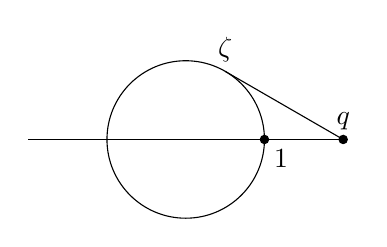
\begin{tikzpicture}[baseline=(O)]
		\draw (0,0) circle [radius=1cm];
		\draw (-2,0) -- (2,0);
		\coordinate (O) at (0:1cm); \coordinate (Q) at (2,0);  \coordinate (Z) at (60:1cm);
		\node[below right] at (O) {$1$}; \draw[fill=black] (O) circle [radius=1.5pt]; 
		\node[above] at (Q) {$q$}; \draw[fill=black] (Q) circle [radius=1.5pt];
		\node[above] at (Z) {$\zeta$};
		\draw (Q) -- (Z);
	\end{tikzpicture} \qquad
	\implies \quad |q-\zeta| > q-1 \geq 1.
	\]
	Jadi $|\Phi_n(q)| = \prod_\zeta |q-\zeta| > q-1$, yang menghasilkan kontradiksi.
\end{proof}

Gelanggang pembagian takkomutatif ditemukan cukup lambat; contoh paling awal yang dapat dilacak ialah temuan W.\ Hamilton pada 1843, yaitu \emph{aljabar kuaternion}. Kelak, ketika membahas aljabar berdimensi hingga, kita akan memberikan beberapa metode sistematis untuk membangun gelanggang pembagian semacam ini.
\begin{example}[Kuaternion]\label{eg:Hamilton-quaternion}\index{siyuanshu@kuaternion (quaternion)}\index[sym1]{H@$\mathbb{H}$}
	Tinjau ruang vektor real dengan basis $1, i, j, k$, yaitu $\mathbb{H} := \R 1 \oplus \R i \oplus \R j \oplus \R k$. Pada ruang ini terdapat perkalian yang terdefinisi dengan baik sehingga $\mathbb{H}$ menjadi gelanggang dan memenuhi sifat-sifat berikut:
	\begin{itemize}
		\item Perkalian $(x,y) \mapsto xy$ merupakan pemetaan bilinear pada $\mathbb{H}$;
		\item $1$ merupakan unsur satuan perkalian, sehingga kita dapat mengidentifikasi $\R$ dengan $\R \cdot 1$ dan membenamkannya ke dalam $Z_{\mathbb{H}}$;
		\item $i^2 = j^2 = -1$;
		\item $ij=k=-ji$.
	\end{itemize}
	Dari sini dapat diturunkan bahwa $k^2 = -1$, $jk=i=-kj$, dan $ki=j=-ik$. Rinciannya diserahkan kepada pembaca. Berdasarkan struktur ruang vektor dan kedua sifat pertama, kita juga menyebut $\mathbb{H}$ sebagai suatu ``$\R$-aljabar''; Definisi \ref{def:algebra-naive} akan memberikan penjelasan terperinci. Selain itu, medan bilangan kompleks $\CC = \R \oplus \R i$ dapat dibenamkan ke dalam $\mathbb{H}$. Berikut ini kita periksa bahwa $\mathbb{H}$ merupakan gelanggang pembagian. Jika operasi konjugasi didefinisikan oleh
	\[ z = a + bi + cj + dk \longmapsto \bar{z} = a - bi -cj -dk \]
	maka berlaku $\overline{z w} = \bar{w}\bar{z}$ dan $z\bar{z} = \bar{z}z = a^2 + b^2 + c^2 + d^2 \in \R$; dari sini diperoleh
	\[ z^{-1} = (z\bar{z})^{-1} \bar{z} = (\underbracket{a^2 + b^2 + c^2 + d^2}_{\neq 0})^{-1} \bar{z}, \quad z \in \mathbb{H} \smallsetminus \{0\}. \]
	Sifat kunci yang digunakan di sini dapat dikembalikan pada fakta bahwa $a^2 + b^2 + c^2 = -1$ tidak mempunyai solusi di dalam medan bilangan real $\R$. Pernyataan yang lebih kuat ialah bahwa $-1$ bukan jumlah kuadrat di dalam $\R$; medan yang memenuhi kondisi terakhir disebut medan real formal, dan merupakan objek yang sangat menarik dalam kajian teori medan, bentuk kuadratik, serta teori model; lihat \cite[\S 9.1]{Feng17}. \index{moxinglun@teori model}
\end{example}

\section{Tinjauan Awal tentang Gelanggang Komutatif}\label{sec:comm-ring-intro}
Teori gelanggang komutatif sangat berbeda dari kasus umum yang nonkomutatif. Di satu pihak, perbedaan ini tampak pada sejumlah konsep dan teknik yang khas bagi gelanggang komutatif; di pihak lain, hal itu bersumber dari kedudukan penting gelanggang komutatif dalam geometri aljabar, teori bilangan aljabar, kombinatorika aljabar, dan bidang-bidang lainnya. Tujuan bagian ini hanyalah memaparkan konsep-konsep dasar, termasuk lokalisasi gelanggang komutatif; kajian yang lebih mendalam akan dibahas dalam bab tersendiri.

Bagian ini hanya membahas gelanggang dengan unsur satuan yang komutatif, sehingga ideal kiri dan ideal kanan tidak perlu dibedakan.

\begin{definition}\label{def:ring-ideal}\index{lixiang!ideal prima (prime ideal)}\index{lixiang!ideal maksimal (maximal ideal)}
	Dalam gelanggang $R$, suatu ideal sejati $I$ disebut
	\begin{compactitem}
		\item \emph{ideal prima}, jika $xy \in I$ mengakibatkan $x \in I$ atau $y \in I$;
		\item \emph{ideal maksimal}, jika $I \neq R$ dan tidak ada ideal yang memuat $I$ secara ketat.
	\end{compactitem}
	Himpunan semua ideal prima dan semua ideal maksimal dalam $R$ masing-masing ditulis $\Spec R$ dan $\MaxSpec R$, serta disebut spektrum prima dan spektrum ideal maksimal dari $R$. \index[sym1]{Spec@$\Spec$}\index[sym1]{MaxSpec@$\MaxSpec$}
\end{definition}
Untuk gelanggang sembarang, konsep kemaksimalan dapat didefinisikan bagi ideal kiri, ideal kanan, dan ideal dua sisi, tetapi kegunaannya tidak seluas dalam kasus komutatif.

\begin{lemma}\label{prop:Spec-pullback}
	Untuk setiap homomorfisme gelanggang $\varphi: R_1 \to R_2$, pemetaan dalam \eqref{eqn:ideal-preimage} membawa ideal prima ke ideal prima; dengan kata lain, $\varphi$ menginduksi peta
	\begin{align*}
		\varphi^\sharp: \Spec R_2 & \longrightarrow \Spec R_1 \\
		I_2 & \longmapsto \varphi^{-1}(I_2).
	\end{align*}
	Dalam bahasa kategori, pemetaan
	\begin{align*}
		R & \longmapsto \Spec R, \\
		[\varphi: R_1 \to R_2] & \longmapsto [\varphi^\sharp: \Spec R_2 \to \Spec R_1]
	\end{align*}
	mendefinisikan fungtor $\Spec: \cate{CRing}^\text{op} \to \cate{Set}$, dengan $\cate{CRing}$ menyatakan kategori gelanggang komutatif.
\end{lemma}
\begin{proof}
	Misalkan $I_2$ adalah ideal prima dari $R_2$. Jika dalam $R_1$ berlaku $xy \in \varphi^{-1}(I_2)$, maka $\varphi(x)\varphi(y) \in I_2$, sehingga salah satu dari $x$ dan $y$ berada dalam $\varphi^{-1}(I_2)$. Jadi $\varphi^{-1}(I_2)$ merupakan ideal prima dari $R_1$. Untuk membuktikan bahwa $\Spec$ memberikan fungtor $\cate{CRing}^\text{op} \to \cate{Set}$, cukup buktikan bagi setiap pasangan homomorfisme $\varphi$, $\psi$ yang dapat dikomposisikan bahwa $(\varphi \circ \psi)^\sharp = \psi^\sharp \circ \varphi^\sharp$; hal ini langsung mengikuti pengamatan bahwa $(\varphi \circ \psi)^{-1} = \psi^{-1} \circ \varphi^{-1}$.
\end{proof}

\begin{remark}
	Secara umum tidak ada hasil yang bersesuaian untuk $\MaxSpec$; lihat Contoh \ref{eg:localization-prime}.
\end{remark}

\begin{proposition}\label{prop:prime-maximal-ideals}
	Misalkan $I$ adalah ideal sejati dari $R$. Maka
	\begin{enumerate}
		\item dalam bijeksi pada Proposisi \ref{prop:2nd-homomorphism-ring}
		\begin{align*}
			\left\{ J \subset R: \text{ideal}, \; J \supset I \right\} & \longrightarrow \{ \bar{J} \subset R/I : \text{ideal} \} \\
			J & \longmapsto \bar{J} := J/I
		\end{align*}
		tersebut, $\bar{J}$ merupakan ideal prima (ideal maksimal) jika dan hanya jika $J$ demikian;
		\item $R/I$ merupakan daerah integral jika dan hanya jika $I$ merupakan ideal prima;
		\item $R/I$ merupakan medan jika dan hanya jika $I$ merupakan ideal maksimal.
	\end{enumerate}
\end{proposition}
\begin{proof}
	Pertama-tama, buktikan pernyataan pertama. Kasus ideal maksimal merupakan akibat langsung dari Proposisi \ref{prop:2nd-homomorphism-ring}. Lema \ref{prop:Spec-pullback} menunjukkan bahwa $\bar{J} \in \Spec R/I \implies J \in \Spec R$. Sekarang misalkan $J \in \Spec R$ dan $J \supset I$. Dalam $R/I$, berlaku $\bar{x}\bar{y} \in \bar{J}$ jika dan hanya jika $xy \in J$, dengan $x,y$ masing-masing merupakan sebarang prabayangan dari $\bar{x}, \bar{y}$. Hal ini menunjukkan bahwa $\bar{J} \in \Spec R/I$.

	Dengan mengambil $J=I$, dua pernyataan yang tersisa masing-masing tereduksi menjadi: $R$ merupakan daerah integral (medan) jika dan hanya jika $\{0\}$ merupakan ideal prima (ideal maksimal). Pernyataan bahwa $\{0\}$ merupakan ideal prima tidak lain berarti $xy=0$ jika dan hanya jika $x=0$ atau $y=0$, tepat seperti definisi daerah integral. Di pihak lain, $\{0\}$ merupakan ideal maksimal jika dan hanya jika satu-satunya ideal sejati dari $R$ adalah $\{0\}$. Ini setara dengan mengatakan bahwa untuk setiap unsur tak nol $x \in R$, ideal $Rx = \lrangle{x}$ harus merupakan seluruh $R$; dengan kata lain, terdapat $y$ sedemikian sehingga $xy=1=yx$.
\end{proof}

\begin{corollary}\label{prop:maximal-implies-prime}
	Setiap ideal maksimal merupakan ideal prima.
\end{corollary}
Konversnya secara umum tidak berlaku karena daerah integral belum tentu merupakan medan.

\begin{proposition}\label{prop:existence-maximal-ideal}
	Misalkan $R$ adalah gelanggang sembarang (tidak harus komutatif). Untuk setiap ideal dua sisi sejati dari $R$, katakanlah $I$, terdapat ideal dua sisi maksimal $\mathfrak{m}$ sedemikian sehingga $\mathfrak{m} \supset I$.
\end{proposition}
Dengan mengambil $I=\{0\}$, kita memperoleh bahwa $R$ mempunyai ideal dua sisi maksimal, asalkan gelanggang ini bukan gelanggang nol. Hasil ini biasanya diterapkan ketika $R$ merupakan gelanggang komutatif.
\begin{proof}
	Semua ideal berikut adalah ideal dua sisi. Dengan Proposisi \ref{prop:2nd-homomorphism-ring}, persoalan segera tereduksi pada kasus $I=\{0\}$, yakni keberadaan ideal maksimal dalam $R$. Pertama-tama, perhatikan bahwa ideal-ideal sejati dari $R$ membentuk suatu himpunan terurut parsial (poset) $(\mathcal{P}, \leq)$: definisikan $I_1 \leq I_2 \iff I_1 \subset I_2$. Dengan demikian, unsur-unsur maksimal dalam $\mathcal{P}$ tepat merupakan ideal-ideal maksimal dari $R$. Berikutnya, kita gunakan Lema Zorn (Teorema \ref{prop:Zorn}) untuk memperoleh unsur maksimal. Pertama-tama, perhatikan bahwa setiap rantai dalam $\mathcal{P}$ (yakni subhimpunan terurut total) mempunyai batas atas. Misalkan $\mathcal{C} \subset \mathcal{P}$ adalah suatu rantai. Dari sifat urutan total diketahui bahwa $J := \bigcup_{I \in \mathcal{C}} I$ juga merupakan ideal dari $R$. Jika $J = R$, maka terdapat $I \in \mathcal{C}$ sedemikian sehingga $1 \in I$, yakni $I = R$, bertentangan dengan definisi $\mathcal{P}$. Jadi $J \in \mathcal{P}$ memberikan batas atas bagi $\mathcal{C}$. Selesai.
\end{proof}

\begin{definition}\label{def:PID}\index{zhulixianghuan@daerah ideal utama (principal ideal domain)}
	Misalkan $I$ adalah ideal dari $R$. Jika terdapat $a \in R$ sedemikian sehingga $I = \lrangle{a} = Ra$, maka $I$ disebut \emph{ideal utama}. Jika semua ideal dari daerah integral $R$ merupakan ideal utama, maka $R$ disebut \emph{daerah ideal utama}.
\end{definition}
Sebagai contoh, gelanggang bilangan bulat $\Z$ merupakan daerah ideal utama (Contoh \ref{eg:Z-pid}).

Berikutnya, kita membahas lokalisasi gelanggang komutatif. Gagasannya adalah menambahkan secara formal invers perkalian bagi unsur-unsur tertentu dalam gelanggang.
\begin{definition}\index{chengxingziji@himpunan bagian multiplikatif (multiplicative subset)}
	Misalkan $R$ adalah gelanggang komutatif. Jika suatu himpunan bagian $S \subset R$ membentuk monoid terhadap perkalian gelanggang, maka $S$ disebut \emph{himpunan bagian multiplikatif} dari $R$.
\end{definition}

Untuk himpunan bagian multiplikatif $S$, \emph{lokalisasi} $R[S^{-1}]$ dikonstruksi sebagai berikut. Pertama-tama, definisikan relasi pada himpunan $R \times S$ dengan \index{jubuhua@lokalisasi (localization)}\index[sym1]{$R[S^{-1}]$}
\[ (r,s) \sim (r',s') \iff \left[ \exists t \in S, \; trs' = tr's \right]. \]
Mudah dibuktikan bahwa $\sim$ merupakan relasi ekuivalensi. Himpunan hasil bagi yang bersesuaian ditulis $R[S^{-1}]$, dan kelas ekuivalensi $[r,s]$ di dalamnya hendaknya dipandang sebagai ``pecahan'' $r/s$. Untuk setiap $t \in S$, berlaku $[r,s]=[rt,st]$. Karena itu, operasi gelanggang berikut merupakan pilihan yang wajar:
\begin{gather*}
	[r,s] + [r',s'] = [rs' + r's, ss'], \\
	[r,s] \cdot [r',s'] = [rr', ss'].
\end{gather*}
Silakan periksa bahwa dengan operasi ini $R[S^{-1}]$ memang merupakan gelanggang komutatif, dengan unsur nol $0 = [0, s]$ dan unsur identitas $1 = [s,s]$, di mana $s \in S$ dapat dipilih sebarang. Dari sini diperoleh
\begin{gather}\label{eqn:localization-zero}
	[r,s]=0 \iff \left[ \exists t \in S, \; tr=0 \right].
\end{gather}
Jadi $R[S^{-1}]$ merupakan gelanggang nol jika dan hanya jika terdapat $s \in S$ sedemikian sehingga $sR=0$. Karena kita mengasumsikan bahwa $R$ mempunyai unsur satuan, hal ini juga setara dengan $0 \in S$; secara umum kasus ini selalu dikecualikan.

Di pihak lain, $r \mapsto [r,1]$ memberikan homomorfisme gelanggang $R \to R[S^{-1}]$. Perhatikan bahwa bayangan setiap $s \in S$ berada dalam $R[S^{-1}]^\times$, dengan invers $[1,s]$. Lokalisasi harus dipandang bersama-sama dengan morfisme $R \to R[S^{-1}]$. Dari sudut pandang teori kategori, konstruksi lokalisasi $R \to R[S^{-1}]$ merupakan cara yang ``paling ekonomis'' untuk membuat unsur-unsur $S$ invertibel, dan dicirikan secara tunggal oleh sifat universal berikut.

\begin{proposition}
	Lokalisasi $R \to R[S^{-1}]$ memenuhi sifat universal berikut: jika suatu homomorfisme gelanggang komutatif $\varphi: R \to A$ memenuhi $\varphi(S) \subset A^\times$, maka terdapat homomorfisme gelanggang tunggal $\varphi[S^{-1}]: R[S^{-1}] \to A$ yang membuat diagram berikut komutatif.
	\[ \begin{tikzcd}
		R \arrow[r, "\varphi"] \arrow[d] & A \\
		R[S^{-1}] \arrow[ru, "{\varphi[S^{-1}]}"'] &
	\end{tikzcd} \]
\end{proposition}
\begin{proof}
	Komutativitas diagram ekuivalen dengan
	\[ [r,s] =[r,1] \cdot [1,s] \xmapsto{\varphi[S^{-1}]} \varphi(r) \varphi(s)^{-1} \in A. \]
	Sebaliknya, mudah dibuktikan bahwa rumus ini memang mendefinisikan homomorfisme gelanggang $R[S^{-1}] \to A$.
\end{proof}

\begin{lemma}\label{prop:localization-units}
	Misalkan $S \subset R$ adalah himpunan bagian multiplikatif dan $0 \notin S$. Unsur $[r,s] \in R[S^{-1}]$ invertibel jika dan hanya jika terdapat $r_1 \in R$ sedemikian sehingga $rr_1 \in S$.
\end{lemma}
\begin{proof}
	Jika $rr_1 \in S$, maka $[r,s] [r_1 s, rr_1] = 1$. Sebaliknya, misalkan terdapat $[r',s']$ sedemikian sehingga $[r,s][r',s'] = 1$. Maka terdapat $t \in S$ sedemikian sehingga $trr' = tss'$, sehingga $r(tr') \in S$.
\end{proof}

Sebagian informasi tentang gelanggang semula $R$ mungkin hilang dalam proses lokalisasi. Dari \eqref{eqn:localization-zero} diketahui bahwa
\[ \Ker \left[ R \to R[S^{-1}] \right] = \left\{r \in R : \exists s \in S, \; sr=0 \right\}. \]
Kita ingin memilih $S$ sebesar mungkin agar $R[S^{-1}]$ merupakan perluasan gelanggang dari $R$. Pembahasan di atas secara natural mengarah pada hasil berikut.
\begin{lemma}
	Misalkan $S \subset R$ adalah himpunan bagian multiplikatif dan $0 \notin S$. Morfisme lokalisasi $R \to R[S^{-1}]$ bersifat injektif jika dan hanya jika $S$ tidak memuat pembagi nol. Di pihak lain, semua unsur bukan pembagi nol dalam $R \smallsetminus \{0\}$ membentuk himpunan bagian multiplikatif dari $R$. Lokalisasi yang bersesuaian ditulis
	\[ R \hookrightarrow \text{Frac}(R), \]
	dan $\text{Frac}(R)$ disebut \emph{gelanggang pecahan total} dari $R$.
\end{lemma}
Jika $R$ merupakan daerah integral, maka $\text{Frac}(R)$ tidak lain adalah lokalisasi pada $S := R \smallsetminus \{0\}$. Dalam hal ini, Lema \ref{prop:localization-units} menunjukkan bahwa $\text{Frac}(R)$ merupakan medan: sesungguhnya, jika $r \neq 0$, maka $[r,s]^{-1} = [s,r]$. Medan ini disebut \emph{medan pecahan} dari $R$. \index{fenshiyu@medan pecahan (field of fractions)}\index[sym1]{Frac(R)@$\text{Frac}(R)$}

\begin{example}
	Medan pecahan dari gelanggang bilangan bulat $\Z$ isomorfik dengan $\Q$: cukup petakan $[r,s] \in \text{Frac}(\Z)$ ke $r/s$.
\end{example}

Berikutnya, kita mempelajari pengaruh lokalisasi terhadap ideal. Tetapkan himpunan bagian multiplikatif $S$ dengan $0 \notin S$. Untuk setiap ideal $I \subset R$, definisikan
\[ I[S^{-1}] := \left\{ [r, s] : r \in I, \; s \in S \right\} \subset R[S^{-1}]. \]
Dari definisi struktur gelanggang pada $R[S^{-1}]$, mudah dibuktikan bahwa $I[S^{-1}]$ sebenarnya merupakan ideal yang dibangkitkan oleh bayangan $I$ di bawah $R \to R[S^{-1}]$. Di pihak lain, dari \eqref{eqn:ideal-preimage} diperoleh peta antarideal
\begin{gather}\label{eqn:ideal-preimage-localization}
	J \mapsto I := \{ r \in R : [r,1] \in J \}
\end{gather}
dengan $J$ suatu ideal dari $R[S^{-1}]$, sedangkan ruas kanan tidak lain adalah prabayangan $J$ di bawah $R \to R[S^{-1}]$. Sekarang perhatikan
\[\begin{tikzcd}
	\left\{ I: \text{ideal dari } R \right\} \arrow[r, yshift=5, "{I \mapsto I[S^{-1}]}"] & \{ J: \text{ideal dari } R[S^{-1}] \}. \arrow[l, yshift=-5, "\eqref{eqn:ideal-preimage-localization}"]
\end{tikzcd}\]
Kita nyatakan bahwa komposisi pada diagram di atas menurut
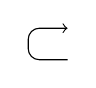
\begin{tikzpicture} [baseline, xscale=0.5, yscale=0.4] \draw[->, rounded corners] (1, 0) -- (0, 0) -- (0, 1) -- (1, 1); \end{tikzpicture}
adalah $\identity$: jelas bahwa $I \mapsfrom J$ mengakibatkan $I[S^{-1}] \subset J$. Di pihak lain, untuk setiap $[r,s] \in J$, berlaku $[r,1] = [r,s][s,1] \in J$, sehingga $r \in I$ dan dengan demikian $J \subset I[S^{-1}]$. Jadi $I \mapsto I[S^{-1}]$ bersifat surjektif, sedangkan \eqref{eqn:ideal-preimage-localization} bersifat injektif. Akan tetapi, jika ideal-ideal yang dibahas tidak dibatasi, maka komposisi pada diagram di atas menurut
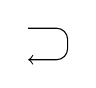
\begin{tikzpicture} [baseline, xscale=0.5, yscale=0.4] \draw[->, rounded corners] (0, 1) -- (1, 1) -- (1, 0) -- (0, 0); \end{tikzpicture}
belum tentu merupakan $\identity$; alasannya akan tampak dari bukti berikut.

\begin{proposition}\label{prop:localization-ideals}
	Misalkan $S$ adalah himpunan bagian multiplikatif dari $R$ dan $0 \notin S$.
	\begin{enumerate}
		\item Untuk setiap ideal $I$, persamaan $I[S^{-1}] = R[S^{-1}]$ berlaku jika dan hanya jika $I \cap S \neq \emptyset$.
		\item Peta $I \mapsto I[S^{-1}]$ menginduksi bijeksi
			\[ \{I \in \Spec R : I \cap S = \emptyset \} \stackrel{1:1}{\longrightarrow} \Spec R[S^{-1}], \]
			dengan invers berupa \eqref{eqn:ideal-preimage-localization} di atas.
		\item Bijeksi tersebut mempertahankan relasi inklusi: $I_1 \subset I_2 \iff I_1[S^{-1}] \subset I_2[S^{-1}]$.
	\end{enumerate}
\end{proposition}
\begin{proof}
	Keanggotaan $1 \in R[S^{-1}]$ berarti bahwa unsur tersebut direpresentasikan oleh suatu kelas $[r, s]$ dengan pembilang di dalam ideal itu dan terdapat $t \in S$ sedemikian sehingga $tr = ts \in S$. Pernyataan pertama langsung diperoleh.

	Sekarang misalkan $I \in \Spec R$ dan $I \cap S = \emptyset$. Dalam $R[S^{-1}]$, berlaku
	\[ [r_1, s_1] [r_2, s_2] \in I[S^{-1}] \iff r_1 r_2 \in I \iff \left( r_1 \in I \; \text{atau} \; r_2 \in I \right), \]
	sehingga $I[S^{-1}]$ merupakan ideal prima. Prabayangannya di bawah $R \to R[S^{-1}]$ sama dengan
	\[ \{r \in R : \exists a \in I, \; s \in S, \quad [r, 1] = [a, s] \} \in \Spec R \quad \because\;\text{Lema \ref{prop:Spec-pullback}}; \]
	Himpunan ini dapat ditulis lebih lanjut sebagai $\{ r \in R : \exists s \in S, \; rs \in I \}$. Karena $S$ tidak beririsan dengan ideal prima $I$, prabayangan tersebut tidak lain adalah $I$. Bersama dengan pembahasan sebelumnya, hal ini membuktikan bahwa $I \mapsto I[S^{-1}]$ merupakan bijeksi pada tingkat ideal prima. Pernyataan mengenai relasi inklusi sudah jelas.
\end{proof}

Bijeksi di atas juga dapat ditulis sebagai
\[ \Spec R[S^{-1}] = \Spec R \smallsetminus \{I \in \Spec R : I \cap S \neq \emptyset \}. \]
Jika spektrum prima $\Spec R$ dipandang sebagai semacam ``ruang'', efek dari $R \mapsto R[S^{-1}]$ dapat dibayangkan sebagai menghilangkan dari $\Spec R$ ``titik-titik'' yang beririsan dengan $S$. Hal ini menjelaskan asal istilah lokalisasi. Karena keterbatasan ruang, makna geometris spektrum prima belum dapat dibahas secara terperinci di sini.

\begin{example}\label{eg:localization-prime}
	Tetapkan $\mathfrak{p} \in \Spec R$. Maka $S := R \smallsetminus \mathfrak{p}$ merupakan himpunan bagian multiplikatif. Dari bijeksi di atas, ideal-ideal prima dari $R_\mathfrak{p} := R[S^{-1}]$ berkorespondensi satu-satu dengan ideal-ideal prima dari $R$ yang termuat dalam $\mathfrak{p}$, sedangkan $\mathfrak{p}[S^{-1}] = \mathfrak{p} R_\mathfrak{p}$ merupakan satu-satunya ideal maksimal dari $R_\mathfrak{p}$, meskipun $\mathfrak{p} \in \Spec R$ yang bersesuaian belum tentu maksimal. Ini merupakan teknik yang lazim dalam teori gelanggang komutatif.
\end{example}

\section{Selingan: Inversi Möbius}\label{sec:Mobius}
Rumus inversi Möbius merupakan alat dasar dalam kombinatorika dan teori bilangan. Ada tiga tujuan pembahasan khusus dalam bagian ini: pertama, melengkapi dengan cepat kasus yang kita perlukan; kedua, memperlihatkan suatu penerapan menarik dari teori gelanggang; dan ketiga, menunjukkan bagaimana rumus inversi Möbius klasik dapat ditata dari sudut pandang yang lebih tinggi dan dirumuskan sebagai perangkat pencacahan pada himpunan terurut parsial. Bagian ini mengikuti pendekatan \cite[\S\S 3.7--3.8]{Stan09} dan menurunkan gagasan dasar inversi Möbius dengan perangkat aljabar.

\begin{definition}\index{pianxuji!lokal berhingga}
	Jika dalam himpunan terurut parsial (poset) tak kosong $(P, \leq)$, untuk setiap $x \leq y$, himpunan bagian $[x,y] := \{ z \in P: x \leq z \leq y \}$ berhingga, maka $(P,\leq)$ disebut \emph{poset lokal berhingga}.
\end{definition}

Untuk poset lokal berhingga $(P, \leq)$, definisikan gelanggang $(I(P, \leq),+,\star)$ sebagai berikut.
\begin{compactitem}
	\item Sebagai grup aditif, gelanggang ini terdiri atas semua fungsi $f: \{(x,y) \in P^2 : x \leq y \} \to \Q$, dengan penjumlahan \linebreak $(f+g)(x,y) = f(x,y) + g(x,y)$;
	\item perkaliannya didefinisikan oleh $(f \star g)(x,y) = \sum_{z: \; x \leq z \leq y} f(x,z) g(z,y)$;
	\item unsur identitas perkaliannya $\delta \in I(P, \leq)$ adalah
	\[ \delta(x,y) = \begin{cases} 1, & x=y \\ 0, & x < y \end{cases} \]
	Ini merupakan notasi yang lazim dalam matematika dan disebut $\delta$ Kronecker. \index{Kronecker@delta Kronecker}
\end{compactitem}
Sifat lokal berhingga memastikan bahwa perkalian pada $I(P, \leq)$ terdefinisi dengan baik. Verifikasi aksioma-aksioma gelanggang sama sekali tidak sulit; sebagai contoh, alasan berlakunya asosiativitas perkalian tepat sama seperti pada perkalian matriks. Perinciannya diserahkan kepada pembaca. Jika dalam definisi tersebut fungsi diperbolehkan mengambil nilai dalam medan sembarang $\Bbbk$, diperoleh apa yang disebut aljabar atas $\Bbbk$, yakni \emph{aljabar insidensi}. Konsep aljabar atas medan akan diperkenalkan dalam \S\ref{sec:algebra-def}, sehingga pembahasannya kita tunda.

Pembalikan relasi urutan menghasilkan $(P, \geq)$ yang tetap merupakan poset lokal berhingga. Dengan mencermati definisi perkalian, diperoleh
\begin{gather}\label{eqn:incidence-ring-op}
	I(P,\geq) = I(P, \leq)^\text{op}.
\end{gather}

\begin{lemma}\label{prop:incidence-ring-inv}
	Misalkan $(P, \leq)$ lokal berhingga. Untuk setiap $f \in I(P, \leq)$, pernyataan-pernyataan berikut ekuivalen:
	\begin{compactitem}
		\item $f$ mempunyai invers kiri terhadap perkalian,
		\item untuk setiap $x \in P$, berlaku $f(x,x) \neq 0$,
		\item $f$ mempunyai invers kanan terhadap perkalian.
	\end{compactitem}
	Khususnya, dalam gelanggang $I(P, \leq)$ berlaku: invertibel dari kiri $\iff$ invertibel $\iff$ invertibel dari kanan.
\end{lemma}
\begin{proof}
	Rumus $g \star f = \delta$ setelah dijabarkan tidak lain adalah
	\begin{align*}
		g(x,x)f(x,x) & =1, \quad x \in P \\
		g(x,y) f(y,y) & = - \sum_{x \leq z < y} g(x,z) f(z,y), \quad x,y \in P, \; x < y.
	\end{align*}
	Jadi berlakunya rumus tersebut mengakibatkan $\forall x \; f(x,x) \neq 0$. Sebaliknya, jika $\forall x \; f(x,x) \neq 0$, rumus di atas mendefinisikan secara tunggal $g(x,y)$ sedemikian sehingga $g \star f = \delta$. Dengan demikian, $f$ invertibel dari kiri jika dan hanya jika $f(x,x) \neq 0$. Kasus invertibel dari kanan diperoleh dengan meninjau $(P,\geq)$ dan menggunakan \eqref{eqn:incidence-ring-op}.
\end{proof}

Untuk poset lokal berhingga $(P,\leq)$, definisikan
\begin{gather*}
	\zeta = \zeta_P \in I(P, \leq), \quad \forall x \leq y, \; \zeta(x,y) = 1, \\
	\mu = \mu_P \in I(P, \leq), \quad \mu := \zeta^{-1}.
\end{gather*}
Invertibilitas $\zeta$ di sini dijamin oleh Lema \ref{prop:incidence-ring-inv}. Fungsi $\mu$ untuk $(P, \leq)$ juga disebut \emph{fungsi Möbius} $\mu$. Penjabaran sifat $\mu \star \zeta = \delta = \zeta \star \mu$ tidak lain adalah
\begin{gather}\label{eqn:Mobius-eq}
	\sum_{z \in [x,y]} \mu(x,z) = \delta(x,y) = \sum_{z \in [x,y]} \mu(z,y).
\end{gather}
Dengan mengingat kembali rumus rekursif dalam bukti Lema \ref{prop:incidence-ring-inv}, diperoleh pula bahwa $\mu$ mengambil nilai dalam $\Z$. Fakta ini penting bagi penerapan berikutnya.\index{Mobius@fungsi Möbius}\index[sym1]{mu@$\mu$}

\begin{proposition}[Rumus Inversi Möbius (Gian-Carlo Rota, 1964)]\label{prop:Mobius-inversion}\index{Mobius@inversi Möbius (Möbius inversion)}
	Misalkan $(A,+)$ adalah grup abelian. Misalkan poset $(P,\leq)$ memenuhi
	\[ \forall x \in P, \quad \{y \in P: y \leq x \} \;\text{berhingga}, \]
	maka $(P,\leq)$ merupakan poset lokal berhingga; selain itu, untuk setiap fungsi $f,g: P \to A$, berlaku
	\[ \forall x,\quad g(x) = \sum_{y \leq x} f(y) \iff \forall x,\quad f(x) = \sum_{y \leq x} g(y) \mu(y,x). \]
\end{proposition}
\begin{proof}
	Syarat tersebut jelas mengakibatkan $(P,\leq)$ lokal berhingga dan semua penjumlahan dalam pernyataan berhingga. Jika rumus pertama berlaku, maka
	\begin{align*}
		\sum_{y \leq x} g(y) \mu(y,x) & = \sum_{z \leq y \leq x} f(z) \mu(y,x) \\
		& = \sum_{z \leq x} \left( \sum_{z \leq y \leq x} \mu(y,x) \right) f(z).
	\end{align*}
	Dengan cara serupa, jika rumus kedua berlaku, maka
	\[ \sum_{y \leq x} f(y) = \sum_{z \leq x} \left( \sum_{z \leq y \leq x} \mu(z,y)\right) g(z). \]
	Gunakan kesamaan dalam $\Z$ yang dinyatakan oleh \eqref{eqn:Mobius-eq} untuk segera memperoleh pernyataan.
\end{proof}

\begin{example}[Polinomial kromatik]
	Bagaimana sebuah peta dapat diwarnai dengan palet yang terdiri atas $q$ warna sehingga distrik/kabupaten yang bertetangga mempunyai warna berbeda? Diagram berikut memperlihatkan contoh Kota Lanzhou, beserta perumusannya kembali dalam teori graf.
	\begin{center}\begin{tikzpicture}
			\node (PIC) at (0,0) {
\includegraphics[width=185pt]{Lanzhou.png}};
			\node (TXT) [right=2em of PIC.east, text width=150pt, align=left] {
				Jika simpul digunakan untuk menyatakan distrik/kabupaten dan pasangan yang bertetangga dihubungkan oleh sisi, maka persoalan semula ekuivalen dengan mewarnai setiap simpul suatu graf planar berhingga $\Gamma$ (dengan $q$ pilihan), sedemikian sehingga kedua ujung setiap sisi mempunyai warna berbeda. Dengan demikian, pewarnaan graf berhingga sembarang dapat dipelajari. Pewarnaan semacam ini disebut “tepat”.
			};
			\node (NOTE) [above=0.5em of TXT.north, text width=120pt, align=left, below delimiter=|] {
				\footnotesize \textcolor{red}{$\bigstar$} Sumber gambar: \href{https://commons.wikimedia.org/wiki/File:Administrative_Division_Lanzhou.svg}{Wikimedia Commons}; garis biru menunjukkan Sungai Kuning.
			};
	\end{tikzpicture}\end{center}

	Tuliskan banyaknya semua pewarnaan tepat dari $\Gamma$ sebagai $M_\Gamma(q)$. Untuk menghitungnya, abaikan dahulu apakah pewarnaan itu tepat. Dengan demikian terdapat tepat $q^{V(\Gamma)}$ pewarnaan, dengan $V(\Gamma)$ menyatakan banyaknya simpul, atau distrik/kabupaten. Kita menyebut $\Gamma'$ suatu subpeta dari $\Gamma$ jika $\Gamma'$ diperoleh dari $\Gamma$ dengan menggabungkan beberapa wilayah administratif, atau dari sudut pandang teori graf, dengan melakukan kontraksi; tuliskan $\Gamma' \leq \Gamma$. Maka semua subpeta dari $\Gamma$ membentuk poset berhingga terhadap $\leq$. Sekarang tampak bahwa
	\[ q^{V(\Gamma)} = \sum_{\Gamma' \leq \Gamma} M_{\Gamma'}(q); \]
	memang, untuk setiap pewarnaan peta, wilayah-wilayah bertetangga yang berwarna sama selalu dapat digabungkan sehingga pewarnaannya menjadi tepat. Dengan menerapkan Proposisi \ref{prop:Mobius-inversion}, diperoleh
	\[ M_\Gamma(q) = \sum_{\Gamma' \leq \Gamma} q^{V(\Gamma')} \mu(\Gamma', \Gamma).  \]
	Dengan memandang $q$ sebagai peubah, polinomial berkoefisien bulat $M_\Gamma(q)$ memberikan suatu invarian aljabar bagi graf $\Gamma$, yang disebut polinomial kromatik dari $\Gamma$. Polinomial ini diperkenalkan oleh Birkhoff dalam penelitiannya tentang masalah empat warna. Dalam fisika statistik, $M_\Gamma(q)$ bersesuaian dengan fungsi partisi model Potts antiferomagnetik keadaan-$q$ pada limit suhu nol; lihat \cite{Sok05}.
\end{example}

Langkah berikutnya adalah menurunkan inversi Möbius klasik; masih diperlukan beberapa tahap.
\begin{lemma}\label{prop:Mobius-prod}
	Misalkan $(P_1, \leq), \ldots, (P_n, \leq)$ adalah poset-poset lokal berhingga. Berikan struktur urutan pada himpunan produk $P := \prod_{i=1}^n P_i$ melalui $(x_i)_{i=1}^n \leq (y_i)_{i=1}^n \iff \forall i\; x_i \leq y_i$. Maka $(P, \leq)$ tetap merupakan poset lokal berhingga dan fungsi Möbiusnya adalah
	\[ \mu_P\left( x, y \right) = \prod_{i=1}^n \mu_{P_i}(x_i, y_i), \quad x=(x_i)_i, \; y=(y_i)_i \in P \]
\end{lemma}
\begin{proof}
	Sangat mudah dilihat bahwa $(P, \leq)$ merupakan poset lokal berhingga. Yang tersisa hanyalah memeriksa, untuk $\mu_P$ yang didefinisikan di atas, persamaan \eqref{eqn:Mobius-eq}. Hal ini tereduksi pada rumus penjumlahan berikut pada $P$:
	\begin{equation*}
		\sum_{\substack{z = (z_i)_i \in P \\ x \leq z \leq y}} = \sum_{x_1 \leq z_1 \leq y_1} \cdots \sum_{x_n \leq z_n \leq y_n}.
	\end{equation*}
\end{proof}

Masih diperlukan suatu perumuman yang mudah. Tinjau keluarga poset lokal berhingga $(P_i, \leq)_{i \in I}$. Andaikan bahwa untuk “hampir semua” indeks $i$ (tepatnya, kecuali paling banyak sejumlah hingga indeks), kita telah menetapkan unsur $\mathring{x}_i \in P_i$. Definisikan \emph{produk terbatas} $P := \Resprod_i P_i$ sebagai
\[ \left\{ (x_i)_i \in \prod_{i \in I} P_i : \text{untuk hampir semua $i$, berlaku}\; x_i = \mathring{x}_i  \right\} \]
Di sini $\Resprod_i P_i$ mewarisi urutan produk pada $\prod_i P_i$: $(x_i)_i \leq (y_i)_i \iff \forall i\; x_i \leq y_i$. Maka $(P, \leq)$ tetap lokal berhingga, dan fungsi Möbiusnya tetap diberikan oleh
\[ \mu_P\left( x, y \right) = \prod_i \mu_{P_i}(x_i, y_i) \]
Untuk hampir semua $i$, berlaku $x_i = y_i = \mathring{x}_i$ dan $\mu_{P_i}(\mathring{x}_i, \mathring{x}_i)=1$, sehingga produk tersebut berhingga. Untuk membuktikan rumus di atas, cukup, bagi setiap $x \leq y$, memeriksa \eqref{eqn:Mobius-eq}. Akan tetapi, rumus itu hanya melibatkan indeks-indeks yang memenuhi $(x_i,y_i) \neq (\mathring{x}_i,\mathring{x}_i)$, dan hanya ada sejumlah hingga indeks $i$ demikian; karena itu persoalan segera tereduksi pada kasus produk berhingga. Sekarang kita dapat menyatakan rumus inversi Möbius klasik.

\begin{example}
	Tinjau himpunan terurut total $(\Z_{\geq 0}, \leq)$. Jelas bahwa $\{y: y \leq x\}$ merupakan himpunan berhingga untuk setiap $x$. Ambil
	\[ \mu(n,m) := \begin{cases} 1, & n-m = 0 \\ -1, & n-m = -1, \\ 0, & \text{kasus lainnya}. \end{cases} \]
	Tanpa perhitungan pun segera tampak bahwa \eqref{eqn:Mobius-eq} berlaku. Inilah fungsi Möbius yang dicari. Dalam kasus khusus ini, pembaca dipersilakan menerjemahkan rumus inversi pada Proposisi \ref{prop:Mobius-inversion} menjadi prinsip pencacahan yang langsung terlihat.
\end{example}

\begin{example}[A.\ F.\ Möbius, 1832]\label{eg:Mobius-classical}
	Sekarang berikan urutan keterbagian pada $\Z_{\geq 1}$: definisikan $n \prec m \iff n \mid m$. Demikian pula, $\{y : y \prec x \}$ berhingga untuk setiap $x$, karena setiap bilangan bulat positif hanya mempunyai sejumlah hingga pembagi. Faktorisasi tunggal bilangan bulat positif memberikan isomorfisme poset:
	\begin{align*}
		\Resprod_{p: \text{prima}} (\Z_{\geq 0}, \leq) & \longrightiso (\Z_{\geq 1}, \prec) \\
		(n_p)_p & \longmapsto \prod_{p: \text{prima}} p^{n_p},
	\end{align*}
	Ruas kiri sesungguhnya merupakan produk terbatas yang telah dijelaskan di atas, dengan $\mathring{x}_p = 0$. Karena itu $\prod_p p^{n_p}$ merupakan produk berhingga dan petanya terdefinisi dengan baik. Menurut versi produk terbatas dari Lema \ref{prop:Mobius-prod}, fungsi Möbius dari $(\Z_{\geq 1}, \prec)$, yang dilambangkan dengan $\mu$, diberikan oleh
	\begin{align*}
		\mu\left( \prod_p p^{n_p}, \prod_p p^{m_p} \right) & = \prod_{p: \text{prima}} \mu_{(\Z_{\geq 0}, \leq)}(n_p, m_p) \\
		& =\begin{cases}
			\prod_{\substack{p: \text{prima}}} (-1)^{n_p - m_p}, & \forall p \quad n_p-m_p \geq -1 \\
			0, & \exists p\quad n_p - m_p < -1.
	\end{cases}\end{align*}
	Tuliskan $\mu(n) := \mu(1,n)$. Maka $\mu(d,n) = \mu(n/d)$, dan rumus di atas memberikan deskripsi langsung
	\[ \mu(n) = \begin{cases}
		(-1)^{(\text{banyaknya faktor prima dari }\; n)}, & n\; \text{bebas kuadrat} \neq 1, \\
		0, & \text{kasus lainnya}.
	\end{cases} \]
	Untuk grup abelian $(A,+)$ dan sebarang fungsi $f, g: \Z_{\geq 1} \to A$, Proposisi \ref{prop:Mobius-inversion} menjadi
	\[ \forall n,\; g(n) = \sum_{d \mid n} f(d) \iff \forall n,\; f(n) = \sum_{d \mid n} g(d) \mu\left( \frac{n}{d} \right). \]

	Inilah rumus inversi Möbius yang dikenal luas. Dalam praktik, rumus ini dibagi lagi menjadi
	\begin{inparaenum}[(a)]
		\item kasus aditif: $A$ diambil sebagai grup aditif $\Z$, $\CC$, dan sebagainya; serta
		\item kasus multiplikatif: $A$ diambil sebagai grup perkalian $\Q^\times$, fungsi rasional tak nol $\Q(X)^\times$, dan sebagainya.
	\end{inparaenum}
	Namun, kerangka teorinya tidak berbeda.
\end{example}

Sekarang tinjau suatu penerapan elementer. Untuk setiap $n \in \Z_{\geq 1}$, fungsi Euler yang dikenal luas $\varphi(n) := |(\Z/n\Z)^\times|$ tidak lain menghitung banyaknya bilangan bulat positif yang $\leq n$ dan relatif prima terhadap $n$. Persamaan berikut selalu berlaku:
\begin{equation}\label{eqn:Euler-phi-sum}\begin{gathered}
	\sum_{d \mid n} \varphi(d) = n, \\
	\sum_{d \mid n} d \mu\left( \frac{n}{d} \right) = \varphi(n).
\end{gathered}\end{equation}
Salah satu penjelasan bagi persamaan pertama adalah sebagai berikut. Nyatakan seluruh $n$ bilangan rasional $\frac{1}{n}, \ldots, \frac{n}{n}$ dalam bentuk pecahan paling sederhana. Maka $\varphi(d)$ tepat merupakan banyaknya unsur yang penyebutnya menjadi $d$; penerapan inversi Möbius segera memberikan persamaan kedua. Semua ini merupakan sifat yang dikenal luas dalam teori bilangan elementer.

\section{Limit dan Pelengkapan Gelanggang}\label{sec:ring-limits}
Dalam bagian ini, setiap $I$ yang muncul merupakan himpunan tak kosong atau kategori tak kosong. Kita akan membahas secara berurutan produk langsung, limit invers $\varprojlim$, dan limit langsung $\varinjlim$, sambil memperkenalkan bahasa topologi himpunan-titik untuk membahas pelengkapan.

\begin{definition}\label{def:ring-direct-product}
	Misalkan $\{R_i : i \in I\}$ suatu keluarga gelanggang. Pada taraf grup aditif, produk langsung $\prod_{i \in I} R_i$ sama seperti dalam Definisi \ref{def:monoid-times}; pada $\prod_{i \in I} R_i$ kita definisikan operasi perkalian dengan
	\[ (r_i)_{i \in I} \cdot (s_i)_{i \in I} = (r_i \cdot s_i)_{i \in I}. \]
	Dengan kata lain, $\prod_{i \in I} R_i$ sekaligus merupakan produk langsung monoid-monoid perkalian, dengan unsur identitas $(1_{R_i})_{i \in I}$. Mudah diperiksa bahwa $\prod_{i \in I} R_i$ memenuhi aksioma-aksioma gelanggang.
\end{definition}

Untuk setiap $j \in I$, peta proyeksi $(r_i)_{i \in I} \mapsto r_j$ merupakan homomorfisme gelanggang dari $\prod_{i \in I} R_i$ ke $R_j$. Produk langsung gelanggang beserta homomorfisme proyeksinya juga memenuhi sifat universal dalam kategori gelanggang (bandingkan Lema \ref{prop:product-monoid-univ-prop}); buktinya sama seperti dalam kasus monoid dan dihilangkan di sini.

\begin{theorem}[Teorema Sisa Tiongkok]\label{prop:CRT}\index{zhongguoshengyudingli@Teorema Sisa Tiongkok (Chinese Remainder Theorem)}
	Misalkan $R$ suatu gelanggang dan $I_1, \ldots I_n$ suatu keluarga ideal. Andaikan bahwa untuk setiap $i \neq j$ berlaku $I_i + I_j = R$. Maka homomorfisme gelanggang
	\begin{align*}
		\varphi: R & \longrightarrow \prod_{i=1}^n R/I_i, \\
		r & \longmapsto \left( r \bmod I_i \right)_{i=1}^n
	\end{align*}
	menginduksi isomorfisme gelanggang $R \big/ (\bigcap_{i=1}^n I_i) \rightiso \prod_{i=1}^n R/I_i$.
\end{theorem}
Selain itu, $\varphi$ juga menginduksi isomorfisme grup $\left( R \big/ (\bigcap_{i=1}^n I_i)\right)^\times \rightiso \prod_{i=1}^n \left(R/I_i\right)^\times$.
\begin{proof}
	Jelas bahwa $\Ker(\varphi) = \bigcap_{i=1}^n I_i$; cukup dibuktikan bahwa $\varphi$ surjektif. Tetapkan $1 \leq i \leq n$. Untuk setiap $j \neq i$, terdapat $r_j \in I_i$ dan $s_j \in I_j$ sedemikian sehingga $r_j + s_j = 1$. Produk $\prod_j$ berikut disepakati dikalikan secara berurutan menurut $j=1,2,\ldots$. Jabarkan $1 = \prod_{j \neq i} (r_j + s_j)$, lalu pisahkan $s := \prod_j s_j \in \prod_{j \neq i} I_j$ dari jumlah semua suku lainnya, yang kita tulis sebagai $r \in I_i$. Dengan demikian diperoleh
	\[ 1 = r + s \in I_i + \prod_{j \neq i} I_j. \]
	Karena itu, bayangan $y_i := s$ dalam $R/I_j$, untuk $j \neq i$, adalah $0$, sedangkan bayangannya dalam $R/I_i$ adalah $1$. Karena untuk setiap $x_1, \ldots, x_n \in R$ berlaku
	\[ \varphi(x_1 y_1 + \cdots + x_n y_n) = (x_i \bmod I_i)_{i=1}^n, \]
	maka $\varphi$ memang surjektif.
\end{proof}

Sekarang ambil $R=\Z$ dan $I_i = a_i \Z$ dalam teorema, dengan $a_i \geq 1$. Jika $a$ adalah kelipatan persekutuan terkecil dari $a_1, \ldots, a_n$, maka $\bigcap_{i=1}^n I_i = a\Z$. Syarat teorema ekuivalen dengan $a_1, \ldots, a_n$ saling koprima secara berpasangan, sedangkan kesimpulannya menyatakan $\Z/a\Z \rightiso \prod_{i=1}^n \Z/a_i\Z$. Inilah bentuk Teorema Sisa Tiongkok dalam teori bilangan elementer.

Sekarang akan dibuktikan bahwa kategori gelanggang $\cate{Ring}$ \index[sym1]{Ring@$\cate{Ring}$} mempunyai limit invers $\varprojlim$ untuk diagram tak kosong. Kita gunakan notasi dari \S\ref{sec:limits} dan tinjau fungtor $\beta: I^\text{op} \to \cate{Ring}$, dengan $I$ suatu kategori kecil (lihat Konvensi \ref{con:U-small}). Demi kemudahan notasi, kita boleh mengandaikan bahwa $I$ sebenarnya merupakan poset kecil tak kosong $(I, \leq)$, sedangkan $\beta$ bersesuaian dengan keluarga gelanggang $\{R_i = \beta(i) \}_{i \in I}$ dan keluarga homomorfisme $\{\varphi_{ij} = \beta(j \to i): R_i \to R_j \}_{i \geq j}$. Keluarga terakhir harus memenuhi syarat kompatibilitas
\[ i \geq j \geq k \implies \varphi_{jk} \varphi_{ij} = \varphi_{ik}: R_i \to R_k. \]

Berikut kita konstruksikan limit invers $\varprojlim \beta = \varprojlim_{i \in I} R_i$ dengan cara yang sama seperti dalam kasus grup pada \S\ref{sec:group-limit}.

\begin{proposition}
	Definisikan subgelanggang dari $\prod_{i \in I} R_i$ dengan
	\[ \varprojlim_{i \in I} R_i := \left\{ (r_i)_{i \in I} \in \prod_{i \in I} R_i : \; \forall i \geq j,\; \varphi_{ij}(r_i) = r_j \right\}. \]
	Maka $\varprojlim_{i \in I} R_i$, bersama keluarga homomorfisme proyeksi $\left( p_j: \varprojlim_{i \in I} R_i \to R_j \right)_{j \in I}$, memenuhi sifat universal berikut. Untuk setiap gelanggang $S$ dan keluarga homomorfisme $(q_j: S \to R_j)_{j \in I}$, jika diagram
	\[ \begin{tikzcd}
		S \arrow[r, "q_i"] \arrow[rd, "q_j"'] & R_i \arrow[d, "\varphi_{ij}"] \\
		&  R_j
	\end{tikzcd} \]
	komutatif untuk setiap pasangan dalam $I$ yang memenuhi $i \geq j$, maka terdapat homomorfisme gelanggang tunggal $\varphi: S \to \varprojlim_{i \in I} R_i$ yang membuat diagram berikut komutatif untuk setiap $j \in I$:
	\[ \begin{tikzcd}
		S \arrow[r, "q_j"] \arrow[d, "{\exists! \, \varphi}"'] & R_j \\
		\varprojlim_{i \in I} R_i \arrow[ru, "p_j"'] &
	\end{tikzcd} \]
\end{proposition}
\begin{proof}
	Karena setiap $\varphi_{ij}$ merupakan homomorfisme gelanggang, mudah dilihat bahwa $\varprojlim_i R_i$ adalah subgelanggang dari $\prod_{i \in I} R_i$. Kekomutatifan diagram ekuivalen dengan pernyataan bahwa, untuk setiap $s \in S$, berlaku $\varphi(s) = (q_i(s))_{i \in I}$; unsur terakhir terletak dalam $\varprojlim_i R_i$ jika dan hanya jika $(S, q_i)$ memenuhi syarat kekomutatifan dalam proposisi. Hal ini menentukan $\varphi$ secara tunggal.
\end{proof}

Untuk kategori kecil umum $I$, konstruksi limit invers $\varprojlim \beta \subset \prod_{i \in \Obj(I)} \beta(i)$ sepenuhnya serupa. Sekarang kita beralih ke pelengkapan sebagai kasus khususnya, dengan mengandaikan $(I, \leq)$ suatu poset terarah ke atas (filtered poset), sebagaimana dalam Definisi \ref{def:filtrant-poset}.

\begin{definition}[Pelengkapan gelanggang]\label{def:ring-completion}\index{wanbeihua@pelengkapan}
	Misalkan $R$ suatu gelanggang dan $(\mathfrak{a}_i)_{i \in I}$ suatu keluarga ideal sejati dua sisi dari $R$, sedemikian sehingga $i \geq j$ mengakibatkan $\mathfrak{a}_i \subset \mathfrak{a}_j$ dan dengan demikian menginduksi peta hasil bagi $\varphi_{ij}: R/\mathfrak{a}_i \to R/\mathfrak{a}_j$. Limit yang bersesuaian, $\varprojlim_{i \in I} R/\mathfrak{a}_i$, bagi $R$ terhadap $(\mathfrak{a}_i)_{i \in I}$, disebut \emph{pelengkapan}.
\end{definition}
Keluarga homomorfisme hasil bagi $R \to R/\mathfrak{a}_i$ menginduksi homomorfisme gelanggang natural $\iota: R \to \varprojlim_i R/\mathfrak{a}_i$, yang kernelnya adalah $\bigcap_i \mathfrak{a}_i$. Dengan menggunakan $R/\Ker(\iota)$ sebagai pengganti $R$, kita selalu dapat mereduksi pada kasus $\Ker(\iota)=\{0\}$; selanjutnya kita andaikan demikian.

Tuliskan $\mathfrak{A}_j$ untuk kernel $\varprojlim_i R/\mathfrak{a}_i \to R/\mathfrak{a}_j$, yakni
\[ \mathfrak{A}_j = \left\{ (r_i)_{i \in I} \in \varprojlim_i R/\mathfrak{a}_i : \; i \leq j \implies r_i=0 \right\}. \]
Sekarang kita perkenalkan konsep \emph{gelanggang topologis}: \index{tuopuhuan@gelanggang topologis, medan topologis, modul topologis} ini berarti suatu gelanggang yang juga memiliki struktur ruang topologis, dengan penjumlahan, negasi, dan perkalian gelanggang semuanya kontinu; khususnya, gelanggang topologis merupakan grup abelian topologis terhadap penjumlahan. Berikan topologi diskret pada setiap $R_i := R/\mathfrak{a}_i$. Maka $\varprojlim_{i \in I} R/\mathfrak{a}_i$ tidak lain adalah pelengkapan bagi grup aditif $R$ terhadap $\{\mathfrak{a}_i\}_{i \in I}$, sebagaimana dalam Definisi \ref{def:group-completion}. Oleh sebab itu, $(\varprojlim_i R_i, +)$ menjadi grup topologis Hausdorff lengkap, dan keluarga ideal $\{\mathfrak{A}_i\}_{i \in I}$ memberikan basis lingkungan di $0$. Lebih lanjut, $\varprojlim_i R_i$ merupakan gelanggang topologis: kontinuitas perkalian langsung mengikuti sifat
\[ (j,k \geq i) \implies \mathfrak{A}_j \cdot \mathfrak{A}_k \subset \mathfrak{A}_i. \]
Jika setiap $R/\mathfrak{a}_i$ merupakan gelanggang berhingga, maka Lema \ref{prop:completion-compactness} menyatakan bahwa $\varprojlim_i R/\mathfrak{a}_i$ kompak.

\begin{remark}\label{rem:ring-completion} \index{a-jintuopu@topologi $\mathfrak{a}$-adik}
	Misalkan $\hat{R} := \varprojlim_i R/\mathfrak{a}_i$. Dari sudut pandang topologis, konstruksi di sini setara dengan menjadikan $(\mathfrak{a}_i)_{i \in I}$ suatu basis lingkungan dari $0 \in R$, sehingga $R$ menjadi gelanggang topologis Hausdorff (lihat \eqref{eqn:top-group-Hausdorff}), lalu, dengan meniru \S\ref{sec:group-limit}, melakukan pelengkapan gelanggang $R$ menjadi $\hat{R}$. Seperti dalam kasus grup, pelengkapan gelanggang berarti suatu homomorfisme gelanggang kontinu $\iota: R \to \hat{R}$ yang dicirikan, hingga isomorfisme tunggal, oleh sifat-sifat berikut:
	\begin{compactenum}[\bfseries {CO}.1]
		\item $\iota: R \to \iota(R)$ merupakan homeomorfisme,
		\item bayangan $\iota$ rapat,
		\item $\hat{R}$ merupakan gelanggang topologis Hausdorff lengkap.
	\end{compactenum}
	Dalam praktik, sering ditetapkan suatu ideal dua sisi $\mathfrak{a}$, lalu dipertimbangkan himpunan terurut total $I = (\Z_{\geq 0}, \leq)$ dan $\mathfrak{a}_i = \mathfrak{a}^{i+1}$; topologi pada $R$ dalam hal ini disebut topologi $\mathfrak{a}$-adik. Jika terdapat $\mathfrak{a}$ yang memberi $R$ topologi $\mathfrak{a}$-adik, kita katakan bahwa $R$ memiliki topologi adik; ini merupakan kelas gelanggang topologis yang lazim. Perhatikan bahwa pilihan $\mathfrak{a}$ tidak tunggal: pembaca dapat memeriksa bahwa untuk setiap $k \in \Z_{\geq 1}$, topologi adik yang ditentukan oleh $\mathfrak{a}^k$ sama dengan yang ditentukan oleh $\mathfrak{a}$.
\end{remark}

\begin{example}\label{eg:Z_p}
	Tinjau gelanggang $R = \Z$ dan keluarga idealnya $\mathfrak{a}_i := p^{i+1} \Z$, dengan $p$ suatu bilangan prima tetap. Pelengkapan yang bersesuaian, $\Z_p$, disebut gelanggang bilangan bulat $p$-adik; gelanggang ini merupakan pelengkapan $\Z$ terhadap topologi $p\Z$-adik (selanjutnya cukup disebut topologi $p$-adik).
\end{example}

\begin{example}\label{eg:Prüfer}
	Ambil himpunan $I := \Z_{> 1}$ dan definisikan poset terarah ke atas melalui keterbagian: $N \prec N' \iff N \mid N'$. Dalam hal ini terdapat homomorfisme hasil bagi $\Z/N'\Z \to \Z/N\Z$. Pelengkapan yang bersesuaian, $\hat{\Z} := \varprojlim_N \Z/N\Z$, disebut gelanggang Prüfer. Sebenarnya $\hat{\Z} \simeq \prod_p \Z_p$, dengan $p$ merentang semua bilangan prima. Alasannya sebagai berikut. Bilangan $N$ mempunyai faktorisasi prima tunggal $N = \prod_p p^{v_p(N)}$, dan untuk setiap $N \prec N'$ terdapat diagram komutatif
	\[ \begin{tikzcd}
		\prod_p (\Z/p^{v_p(N')}\Z ) \arrow[twoheadrightarrow, d] \arrow[r, "\sim"] & \Z/N'\Z \arrow[twoheadrightarrow, d] \\
		\prod_p (\Z/p^{v_p(N)}\Z ) \arrow[r, "\sim"'] & \Z/N\Z
	\end{tikzcd} \]
	dengan isomorfisme-isomorfisme horizontal berasal dari Teorema Sisa Tiongkok dan homomorfisme-homomorfisme vertikal merupakan peta hasil bagi. Perbandingan kedua pelengkapan memberikan $\prod_p \Z_p \rightiso \hat{\Z}$.
\end{example}

Gelanggang $\Z_p$ merupakan contoh khas pelengkapan. Karena penerapannya luas, berikut ini kita kaji lebih lanjut sifat-sifat $\Z_p$, sekaligus memperagakan beberapa teknik dasar dalam teori gelanggang komutatif. Pertama, perhatikan bahwa konstruksi $\varprojlim$ mengakibatkan
\begin{align*}
	p^{n+1} \Z_p & = \left\{ (x_i)_{i \geq 0} : x_i \in p^{n+1} \cdot \Z/p^{i+1}\Z \right\} \\
	& = \left\{ (x_i)_{i \geq 0} : i \leq n \implies x_i=0 \right\} = \Ker\left[ \Z_p \stackrel{p_n}{\twoheadrightarrow} \Z/p^{n+1}\Z \right].
\end{align*}
Dengan demikian, $\Z_p/p^{n+1}\Z_p \rightiso \Z/p^{n+1}\Z$. Hal ini juga mengakibatkan $p\Z_p$ merupakan ideal maksimal. Selain itu, perhatikan bahwa $p$ bukan pembagi nol dalam $\Z_p$: jika $(x_i)_i \neq 0$, pilih $n$ sedemikian sehingga $x_{n-1} \neq 0$. Maka harus berlaku $x_n \notin p^n \Z/p^{n+1}\Z$, sehingga $px_n \neq 0$.

Untuk setiap $x = \left( x_i \in \Z/p^{i+1}\Z \right)_{i \geq 0} \in \Z_p$, pengamatan di atas memungkinkan kita mendefinisikan
\[ v_p(x) := \sup\{n: x \in p^n\Z_p \} = \inf\{n : x_n \neq 0\}. \]
Fungsi $v_p: \Z_p  \to \Z_{\geq 0} \sqcup \{\infty\}$ disebut valuasi $p$-adik.

\begin{proposition}\label{prop:p-adic}\index[sym1]{Z_p}
	Untuk setiap bilangan prima $p$, sifat-sifat berikut berlaku.
	\begin{enumerate}
		\item $\Z_p$ merupakan daerah integral, dan $v_p(x) = \infty \iff x=0$.
		\item Untuk setiap $x,y \in \Z_p$,
			\begin{align*}
				v_p(xy) & = v_p(x) + v_p(y), \\
				v_p(x+y) & \geq \min\{v_p(x), v_p(y)\}, \quad \text{(ketaksamaan segitiga kuat)}.
			\end{align*}
		\item Unsur $x \in \Z_p$ invertibel jika dan hanya jika $v_p(x)=0$.
		\item $\Z_p$ merupakan gelanggang ideal utama, dan setiap ideal tak nol di dalamnya berbentuk $p^n \Z_p = \{x \in \Z_p: v_p(x) \geq n \}$.
  \end{enumerate}
\end{proposition}
\begin{proof}
	Tuliskan $W := \Z_p$. Argumen selanjutnya hanya memerlukan definisi $v_p(x) = \sup\{n: x \in p^n W\}$ dan sifat-sifat yang telah diamati:
	\begin{inparaenum}[(a)]
		\item $W \rightiso \varprojlim_{n \geq 0} W/p^{n+1}W$;
		\item $p$ bukan pembagi nol dalam $W$;
		\item $W/pW$ merupakan medan.
	\end{inparaenum}

	Pertama, $v_p(x)=\infty$ ekuivalen dengan $x \in \bigcap_{n \geq 0} p^{n+1}W$, tetapi (a) mengakibatkan bahwa dalam hal ini $x=0$. Selanjutnya kita buktikan bahwa $W$ merupakan daerah integral. Jika $x,y \in W$ keduanya tak nol, langkah sebelumnya memungkinkan kita menulis $x=p^{v_p(x)} x'$ dan $y=p^{v_p(y)} y'$ dengan $x',y' \notin pW$. Berkat (b), persoalan tereduksi pada pembuktian bahwa $x'y' \neq 0$. Namun, $W/pW$ merupakan medan, sehingga $x'y' \notin pW$ dan khususnya $x'y' \neq 0$.

	Berikut kita buktikan kedua sifat $v_p$. Sekali lagi, tuliskan $x = p^{v_p(x)} x'$ dan $y = p^{v_p(y)} y'$. Tanpa mengurangi keumuman, andaikan $v_p(x) \geq v_p(y)$. Maka $x+y \in p^{v_p(y)}W$, sehingga $v_p(x+y) \geq \min\{ v_p(x), v_p(y)\}$. Selain itu, $x'y' \notin pW$ mengakibatkan $v_p(xy) = v_p(x) + v_p(y)$.

	Misalkan $x \in W^\times$. Dengan meninjau bayangannya modulo $pW$, diperoleh $v_p(x) = 0$. Sebaliknya, andaikan $x \in W \smallsetminus pW$. Dari (c), terdapat $a \in W$ sedemikian sehingga $ax \equiv 1 \pmod{pW}$. Karena itu, tanpa mengurangi keumuman kita dapat mengandaikan $x \equiv 1 \pmod{pW}$. Tuliskan $x = 1-t$, dengan $v_p(t) \geq 1$. Dalam gelanggang topologis Hausdorff $W$ berlaku kesamaan
	\[ x(1 + t + \cdots + t^N) = (1 - t)(1 + t + \cdots + t^N) = 1 - t^{N+1}. \]
	Ketika $N \to \infty$, ruas kanan menuju $1$. Jika dapat dibuktikan bahwa $y_N := 1+ t +\cdots + t^N$ juga konvergen, limitnya memberikan $x^{-1}$. Untuk itu, cukup diperhatikan bahwa apabila $N' \geq N$, dalam penjumlahan $y_{N'}$, suku-suku setelah $t^N$ tidak memengaruhi kelasnya modulo $p^N W$.

	Terakhir, kita buktikan pernyataan tentang ideal. Andaikan $I$ suatu ideal tak nol dalam $W$. Definisikan $n := \min\{v_p(x) : x \in I\}$; dengan demikian $I \subset p^n W$. Ambil unsur tak nol $x = p^n y \in I$ dengan $v_p(x)=n$. Maka $y$ harus invertibel, sehingga $p^n W = xW \subset I$. Terbuktilah pernyataan tersebut.
\end{proof}

Lokalisasi gelanggang $\Z_p$ pada himpunan multiplikatif $\{1,p,p^2,\ldots\}$, yaitu $\Z_p[\frac{1}{p}] =: \Q_p$, disebut \emph{medan bilangan $p$-adik}. Dari karakterisasi unsur invertibel di atas, diketahui bahwa $\Q_p = \text{Frac}(\Z_p)$; setiap unsur tak nolnya dapat ditulis secara tunggal sebagai $p^a t$, dengan $t \in \Z_p^\times$ dan $a \in \Z$. Valuasi $v_p$ juga memiliki perluasan natural ke $\Q_p$: $v_p(p^a t) = a$. Pembaca dipersilakan memeriksa bahwa ketaksamaan pada Proposisi \ref{prop:p-adic} tetap berlaku pada $\Q_p$. Di sisi lain, $\Q_p$ juga dapat dipandang sebagai pelengkapan medan $\Q$ terhadap valuasi $v_p\big|_\Q$, sehingga dapat dikonstruksi secara langsung; hal ini akan dibahas secara terperinci dalam \S\ref{sec:valued-field}.

Sekarang kita beralih ke kajian $\varinjlim$. Tinjau suatu kategori kecil $I$ dan fungtor $\alpha: I \to \cate{Ring}$. Untuk $I$ yang merupakan kategori terarah ke atas (filtered category), kita akan mendefinisikan limit langsung $\varinjlim \alpha$, sebagaimana dalam Definisi \ref{def:filtrant-cat}. Dalam penerapan, $I$ sering kali merupakan poset terarah ke atas, tetapi untuk menonjolkan peranan syarat keterarahan ke atas, kita akan menangani kasus umum secara lengkap. Ingat bahwa dalam $I$, untuk setiap morfisme $f: i \to j$, terdapat homomorfisme gelanggang yang bersesuaian, $\alpha(f): \alpha(i) \to \alpha(j)$.

Andaikan kategori $I$ terarah ke atas. Dalam Contoh \ref{eg:set-limits}, pada $\bigsqcup_{i \in \Obj(I)} \alpha(i)$ kita telah, melalui \eqref{eqn:filtrant-equiv}, mendefinisikan relasi ekuivalensi $\sim$. Dengan demikian, dalam $\cate{Set}$, $\varinjlim \alpha$ direalisasikan sebagai himpunan hasil bagi $\bigsqcup_{i \in \Obj(I)} \alpha(i) \big/ \sim$. Untuk setiap $j \in \Obj(I)$ terdapat peta
\[ \iota_j: \alpha(j) \to \bigsqcup_{i \in \Obj(I)} \alpha(i) \xrightarrow{\text{peta hasil bagi}} \varinjlim \alpha. \]

Sekarang akan dibuktikan bahwa himpunan hasil bagi $\varinjlim \alpha$ mempunyai struktur gelanggang tunggal sedemikian sehingga, untuk setiap $f: j \to j'$,
\begin{equation}\label{eqn:filtrant-lim-ring} \begin{tikzcd}[row sep=small]
	\alpha(j) \arrow[rd, "\iota_j"'] \arrow[rr, "\alpha(f)"] & & \alpha(j') \arrow[ld, "{\iota_{j'}}"] \\
	& \varinjlim \alpha &
\end{tikzcd}\end{equation}
merupakan diagram komutatif dalam $\cate{Ring}$.

Kita gunakan notasi dari konstruksi limit langsung terarah ke atas pada himpunan. Definisikan struktur gelanggang pada $\varinjlim \alpha$ sebagai berikut. Untuk dua kelas ekuivalensi sembarang $[r_i]$ dan $[r'_j]$, definisi kategori terarah ke atas menjamin adanya panah dari $i,j$ menuju suatu $k \in \Obj(I)$, serta unsur $r_k, r'_k \in \alpha(k)$, sedemikian sehingga $[r_i] = [r_k]$ dan $[r'_j] = [r'_k]$. Dalam \eqref{eqn:filtrant-lim-ring}, dengan mengambil $f = \identity: k \to k$, tampak bahwa $[r_i][r'_j]$ hanya mungkin didefinisikan sebagai $[r_k r'_k]$. Cara yang sama membuktikan bahwa perkalian ini terdefinisi dengan baik dan memberikan struktur gelanggang (unsur identitasnya adalah kelas ekuivalensi dari $1 \in \alpha(i)$, dengan $i$ sembarang) yang membuat \eqref{eqn:filtrant-lim-ring} selalu komutatif. Ketika membandingkan perkalian yang diperoleh dari berbagai pilihan, kita selalu dapat bergerak cukup “jauh” dalam kategori $I$ untuk menghilangkan semua ketakpastian; inilah inti Definisi \ref{def:filtrant-cat}. Dengan demikian, pernyataan tersebut telah terbukti.

\begin{proposition}\label{prop:ring-filtrant-limit}
	Untuk kategori kecil terarah ke atas $I$ dan $\alpha: I \to \cate{Ring}$ seperti di atas, gelanggang $\varinjlim \alpha$ bersama keluarga homomorfisme $\iota_j: \alpha(j) \to \varinjlim \alpha$ membentuk, dalam kategori $\cate{Ring}$, limit langsung $\varinjlim \alpha$.
\end{proposition}
\begin{proof}
	Jika struktur gelanggang dilupakan, $\varinjlim \alpha$ sebagai himpunan merupakan limit langsung dari $\alpha(i)$ dalam $\cate{Set}$. Karena itu, untuk setiap gelanggang $R$ dan keluarga homomorfisme $\left( \iota'_j: \alpha(j) \to R \right)_{j \in \Obj(I)}$ sedemikian sehingga diagram
	\[ \begin{tikzcd}[row sep=tiny]
		\alpha(i) \arrow[dd, "\alpha(f)"'] \arrow[rd, "\iota'_i"] & \\
		& R \\
		\alpha(j) \arrow[ru, "\iota'_j"'] &
		\end{tikzcd} \qquad (f: i \to j) \]
	selalu komutatif, terdapat peta himpunan tunggal $\varphi: \varinjlim \alpha \to R$ sedemikian sehingga
	\[ \begin{tikzcd}
		\alpha(i) \arrow[r, "\iota_i"] \arrow[rd, "\iota'_i"'] & \varinjlim \alpha \arrow[d, "\varphi"] \\
		& R
	\end{tikzcd} \qquad i \in \Obj(I) \]
	selalu komutatif. Sebenarnya $\varphi([r_i]) = \iota'_i(r_i)$; yang perlu dibuktikan ialah bahwa $\varphi$ merupakan homomorfisme gelanggang. Argumennya serupa dengan sebelumnya: gunakan syarat kategori terarah ke atas bersama sifat keluarga homomorfisme gelanggang $\iota'_j: \alpha(j) \to R$. Perinciannya diserahkan kepada pembaca.
\end{proof}

Di atas selalu diandaikan bahwa $I$ tak kosong. Sekarang kita lengkapi kasus ketika $I$ merupakan kategori kosong. Perhatikan bahwa $\varinjlim$ kosong tidak lain adalah objek awal dalam kategori. Dari \eqref{eqn:ring-struct-morphism} dan pembahasan sesudahnya, segera diperoleh hasil sederhana tetapi penting berikut.
\begin{proposition}
	Gelanggang bilangan bulat $\Z$ merupakan objek awal dalam kategori gelanggang $\cate{Ring}$.
\end{proposition}

Pembaca mungkin bertanya: apakah semua $\varinjlim$ kecil selalu ada dalam kategori gelanggang? Karena bab ini hanya membahas gelanggang dengan unsur satuan yang tak nol, jawabannya negatif. Contoh berikut menunjukkan bahwa koekualiser dari sepasang homomorfisme $f,g: R \to S$ belum tentu ada. Tinjau gelanggang polinomial $R = \CC[X]$ dan $S = \CC$, dengan homomorfisme $f: P \mapsto P(0)$ dan $g: P \mapsto P(1)$, di mana $P \in \CC[X]$. Jika terdapat homomorfisme gelanggang $h: S \to T$ yang memenuhi $hf=hg$, ambil $P(X)=-X$; maka $h(1) = h(P(0)-P(1)) = 0$, bertentangan dengan $h(1)=1$.

\section{Dari Gelanggang Monoid ke Gelanggang Polinomial}\label{sec:polynomial-ring}
Pembaca tentu sudah mengenal gelanggang polinomial berkoefisien rasional $\Q[X] = \left\{ a_0 + a_1 X + \cdots + a_n X^n : n \geq 0, \; a_i \in \Q \right\}$. Sebagai ruang vektor atas $\Q$, gelanggang ini mempunyai basis $\{ X^i : i \geq 0 \}$, sedangkan perkaliannya tidak lain merupakan perumusan kembali penjumlahan pada monoid $(\Z_{\geq 0}, +)$. Mengganti monoid tersebut dengan monoid sembarang menghasilkan perumuman berikut. Selanjutnya tetapkan suatu gelanggang $R$ dan tinjau polinomial dengan koefisien di dalamnya.

\begin{definition}\label{def:monoidal-ring}\index{yaobanqunhuan@gelanggang monoid}\index[sym1]{$R[M]$}
	Misalkan $M$ suatu monoid. \emph{Gelanggang monoid} $R[M]$ didefinisikan sebagai berikut: unsur-unsurnya adalah barisan dalam himpunan produk $R^M$ yang berbentuk $(r_m)_{m \in M}$, dengan hanya berhingga banyak suku tak nol. Lazimnya, $(r_m)_{m \in M}$ ditulis secara formal sebagai kombinasi linear berhingga atas $R$,
	\[ f = \sum_{m \in M} r_m m, \]
	dengan $r_m$ disebut koefisien $m$ dalam $f$. Penjumlahan dan perkalian pada $R[M]$ masing-masing didefinisikan oleh
	\begin{align*}
		\left( \sum_m r_m m \right) + \left( \sum_m s_m m \right) & = \sum_m (r_m + s_m) m, \\
		\left( \sum_m r_m m \right) \cdot \left( \sum_m s_m m \right) & = \sum_m \left( \sum_{\substack{x, y \in M \\ xy=m}} r_x s_y \right) m,
	\end{align*}
	Mudah dilihat bahwa setiap jumlah di sini hanya mempunyai berhingga banyak suku tak nol, sehingga operasi-operasi tersebut terdefinisi dengan baik.
\end{definition}

Tidak sulit memeriksa bahwa $R[M]$ memenuhi aksioma-aksioma gelanggang. Unsur nolnya adalah $0 = \sum_m 0 \cdot m$ dan unsur identitasnya adalah $1 = 1_R \cdot 1_M$; di sini $1_R$ dan $1_M$ masing-masing menyatakan unsur identitas $R$ dan $M$. Sebenarnya, operasi perkalian pada $R[M]$ ditentukan secara tunggal oleh $(rm) \cdot (r'm') = rr' (mm')$ dan hukum distributif ($r,r' \in R$, $m, m' \in M$). Asosiativitas perkalian cukup diperiksa pada suku berbentuk $rm$.

Perhatikan bahwa gelanggang monoid mempunyai homomorfisme natural
\[\begin{tikzcd}[row sep=tiny]
	M \arrow[r, "\text{monoid}"] & (R[M], \cdot) \\
	m \arrow[mapsto, r] \arrow[phantom, u, sloped, "\in" description] & 1 \cdot m \arrow[phantom, u, sloped, "\in" description]
\end{tikzcd} \quad
\begin{tikzcd}[row sep=tiny]
	R \arrow[r, "\text{gelanggang}"] & R[M] \\
	r \arrow[mapsto, r] \arrow[phantom, u, sloped, "\in" description] & r \cdot 1. \arrow[phantom, u, sloped, "\in" description]
\end{tikzcd}\]
Keduanya injektif, dan bayangan keduanya saling komutatif terhadap perkalian dalam $R[M]$, yakni $(r \cdot 1)(1 \cdot m) = (1 \cdot m)(r \cdot 1)$ (meskipun $R$ dan $M$ sendiri tidak harus komutatif). Hal ini memberikan penjelasan melalui sifat universal bagi konstruksi $R[M]$.

\begin{proposition}\label{prop:monoid-ring-universal}
	Gelanggang monoid dicirikan oleh sifat universal berikut. Untuk setiap gelanggang $S$, homomorfisme monoid $f: M \to (S, \cdot)$, dan homomorfisme gelanggang $g: R \to S$, jika bayangan $f$ dan $g$ saling komutatif terhadap perkalian dalam $S$, maka terdapat homomorfisme gelanggang tunggal $\varphi: R[M] \to S$ sedemikian sehingga $f$ dan $g$ masing-masing sama dengan komposisi $M \to R[M]$ dan $R \to R[M]$ dengan $\varphi$.
\end{proposition}
\begin{proof}
	Satu-satunya pilihan adalah $\varphi(rm) = g(r)f(m)$. Perinciannya diserahkan kepada pembaca.
\end{proof}

Jika pembaca bersedia menggunakan lebih dahulu istilah dalam \S\ref{sec:algebra-def}, khususnya Proposisi \ref{prop:algebra-as-homomorphism}, maka apabila $R$ komutatif, homomorfisme $R \hookrightarrow R[M]$ di atas memberi $R[M]$ struktur aljabar atas $R$. Karena itu, $R[M]$ juga disebut \emph{aljabar monoid} atas gelanggang komutatif $R$.

\begin{definition}\label{def:group-ring}\index{qunhuan@gelanggang grup, aljabar grup (group ring, group algebra)}
	Jika $M$ merupakan grup, gelanggang $R[M]$ disebut \emph{gelanggang grup} dari $M$ atas $R$. Jika $R$ komutatif, gelanggang ini juga disebut \emph{aljabar grup} atas $R$.
\end{definition}

Gelanggang grup merupakan bahasa dasar teori representasi. Sekarang kita kembali pada pengantar di awal bagian ini, yang juga merupakan salah satu konstruksi paling mendasar dalam teori gelanggang: gelanggang polinomial.
\begin{definition}[Gelanggang polinomial]\index{duoxiangshihuan@gelanggang polinomial (polynomial ring)} \index[sym1]{$R[X,\ldots]$}
	Untuk suatu himpunan $\mathcal{X}$, ambil $(\mathbf{M}(\mathcal{X}), \cdot)$ sebagai monoid komutatif bebas pada $\mathcal{X}$ (Definisi \ref{def:free-comm-monoid}; perhatikan bahwa di sini digunakan notasi perkalian). Maka $R[\mathcal{X}] := R[\mathbf{M}(\mathcal{X})]$ disebut gelanggang polinomial atas $R$ dengan himpunan peubah $\mathcal{X}$, dan dilengkapi peta natural $\mathcal{X} \to R[\mathcal{X}]$. Jika $\mathcal{X} = \{X, Y, \ldots\}$, ditulis pula $R[\mathcal{X}] = R[X, Y, \ldots]$.
\end{definition}
Jika $R$ komutatif, $R[\mathcal{X}]$ juga disebut aljabar polinomial dengan himpunan peubah $\mathcal{X}$, dan seterusnya.

\begin{proposition}\label{prop:polynomial-ring-universal}
	Sifat universal berikut mencirikan $R[\mathcal{X}]$ dan $\mathcal{X} \to R[\mathcal{X}]$. Untuk setiap gelanggang $S$, peta $f: \mathcal{X} \to S$, dan homomorfisme gelanggang $g: R \to S$, jika bayangan $f$ dan $g$ saling komutatif terhadap perkalian dalam $S$, dan bayangan $f$ juga komutatif terhadap perkalian, maka terdapat homomorfisme gelanggang tunggal $\varphi: R[\mathcal{X}] \to S$ sedemikian sehingga $f$ dan $g$ masing-masing sama dengan komposisi $\mathcal{X} \to R[\mathcal{X}]$ dan $R \to R[\mathcal{X}]$ dengan $\varphi$.
\end{proposition}
\begin{proof}
	Ini merupakan gabungan sifat universal gelanggang monoid dan sifat universal $\mathbf{M}(\mathcal{X})$.
\end{proof}

Bayangan peta $\mathbf{M}(\mathcal{X}) \to R[\mathcal{X}]$ disebut monomial. Untuk setiap $f \in R[\mathcal{X}]$, koefisien $1 \in \mathbf{M}(\mathcal{X})$ dalam $f$ disebut suku konstan dari $f$. Perhatikan beberapa sifat berikut:
\begin{itemize}
	\item $R[\mathcal{X}]$ komutatif jika dan hanya jika $R$ komutatif;
	\item jika $R$ merupakan daerah integral komutatif, maka $R[\mathcal{X}]$ juga demikian;
	\item setiap homomorfisme gelanggang $R \to R'$ dan peta $\mathcal{X} \to \mathcal{X}'$ menginduksi homomorfisme natural $R[\mathcal{X}] \to R'[\mathcal{X}']$;
	\item untuk setiap himpunan $\mathcal{X}$ dan $\mathcal{Y}$ terdapat isomorfisme natural $R[\mathcal{X}][\mathcal{Y}] = R[\mathcal{Y}][\mathcal{X}] = R[\mathcal{X} \sqcup \mathcal{Y}]$.
\end{itemize}
Sebagai contoh untuk sifat terakhir, kita dapat memberikan isomorfisme yang jelas secara langsung ataupun menjelaskannya dengan sifat universal. Untuk setiap gelanggang $S$, memberikan homomorfisme gelanggang $\varphi: R[\mathcal{X}][\mathcal{Y}] \to S$ ekuivalen dengan memberikan peta $\mathcal{Y} \to S$ dan homomorfisme gelanggang $R[\mathcal{X}] \to S$ yang bayangannya saling komutatif. Dengan sekali lagi menerapkan sifat universal pada yang terakhir, data ini tidak lain adalah peta $\mathcal{Y} \to S$ dan $\mathcal{X} \to S$ (yakni peta $\mathcal{X} \sqcup \mathcal{Y} \to S$), serta homomorfisme gelanggang $R \to S$, sedemikian sehingga ketiga bayangannya saling komutatif terhadap perkalian. Tepat inilah sifat universal $R[\mathcal{X} \sqcup \mathcal{Y}]$.

\begin{definition}[Medan fungsi rasional]\index{youlihanshuyu@medan fungsi rasional (field of rational functions)}\index[sym1]{$F(X,\ldots)$}
	Jika $F$ suatu medan, gelanggang polinomial $F[\mathcal{X}]$ mempunyai medan pecahan $F(\mathcal{X})$. Medan ini, yang dipandang sebagai medan atas $F$ dengan himpunan peubah $\mathcal{X}$, disebut \emph{medan fungsi rasional}. Jika $\mathcal{X} = \{X, Y, \ldots\}$, ditulis pula $F(\mathcal{X}) = F(X, Y, \ldots)$.
\end{definition}
Seperti polinomial di atas, fungsi rasional di sini sebenarnya bukan fungsi; istilah tersebut hanya merupakan konvensi. Nanti akan terlihat bahwa deret pangkat dalam analisis matematika (misalnya $e^X = \sum_{n \geq 0} X^n/n!$) juga mempunyai konstruksi formal.

Kita uraikan lebih lanjut $R[\mathcal{X}]$. Ingat bahwa setiap unsur $\mathbf{M}(\mathcal{X})$ dapat ditulis secara tunggal sebagai $X_1^{a_1} \cdots X_n^{a_n}$, dengan $X_1, \ldots, X_n \in \mathcal{X}$ dan $a_1, \ldots, a_n \geq 0$ (tanpa memperhitungkan urutan). Karena itu, unsur $R[\mathcal{X}]$ merupakan kombinasi linear dari ``monomial'' berbentuk $X_1^{a_1} \cdots X_n^{a_n}$ (dengan koefisien dalam $R$). Inilah versi abstrak polinomial, dengan $\mathcal{X}$ tepat sebagai himpunan peubahnya. Selanjutnya kita khususkan pada kasus $\mathcal{X} = \{X_1, \ldots, X_n\}$. Dalam hal ini $R[\mathcal{X}] = R[X_1, \ldots, X_n]$ merupakan gelanggang polinomial dalam $n$ peubah, dan unsur-unsurnya ditulis dengan notasi klasik $f = f(X_1, \ldots, X_n)$. Unsur gelanggang $R[X_1, \ldots, X_n]$ berbentuk
\[ f = \sum_{a_1, \ldots, a_n \in \Z_{\geq 0}} c_{a_1, \ldots, a_n} X_1^{a_1} \cdots X_n^{a_n}. \]

Karena indeksnya agak rumit, kita sekalian memperkenalkan notasi \emph{multiindeks} yang praktis:
\begin{align*}
	\bm{a} & := (a_1, \ldots, a_n), \quad a_1, \ldots, a_n \in \Z_{\geq 0}, \\
	|\bm{a}| & := a_1 + \cdots + a_n, \\
	c_{\bm{a}} & := c_{a_1, \ldots, a_n}, \\
	\bm{X}^{\bm{a}} & := X_1^{a_1} \cdots X_n^{a_n}.
\end{align*}
Dengan notasi ini, \emph{derajat total} polinomial $f$ didefinisikan sebagai $\deg f := \max\left\{ |\bm{a}| : c_{\bm{a}}\neq 0 \right\}$. Jika $f$ memenuhi $c_{\bm{a}} \neq 0 \iff |\bm{a}|=m$, maka $f$ disebut \emph{polinomial homogen} berderajat $m$.

Untuk multiindeks $\bm{a} = (a_1, \ldots, a_n)$ dan $\bm{b} = (b_1, \ldots, b_n)$, tetapkan $\bm{a} + \bm{b} := (a_1 + b_1, \ldots, a_n + b_n)$. Maka perkalian dalam $R[X_1, \ldots, X_n]$ mempunyai bentuk ringkas
\begin{equation}\label{eqn:polynomial-multiplication}
	\left( \sum_{\bm{a}'} c'_{\bm{a}'} \bm{X}^{\bm{a}'} \right) \cdot \left( \sum_{\bm{a}''} c''_{\bm{a}''} \bm{X}^{\bm{a}''} \right) = \sum_{\bm{a}} \; \underbracket{ \left( \sum_{\bm{a}' + \bm{a}'' = \bm{a}} c'_{\bm{a}'} c''_{\bm{a}''} \right) }_{\text{jumlah berhingga}} \bm{X}^{\bm{a}}.
\end{equation}

Jika $n=1$, kita kembali pada gelanggang polinomial satu peubah $R[X]$ yang dikenal luas. Polinomial berbentuk $X^n + a_{n-1} X^{n-1} + \cdots + a_0 \in R[X]$ ($n \geq 1$) disebut \emph{polinomial monik}. Operasi turunan dalam kalkulus dapat didefinisikan secara formal pada $R[X]$. \index{shouyiduoxiangshi@polinomial monik (monic polynomial)}\index{daoshu@turunan (derivative)}
\begin{proposition}\label{prop:polynomial-derivation}
	Peta
	\begin{align*}
		\partial: R[X] & \longrightarrow R[X] \\
		f(X) = \sum_{k \geq 0} a_k X^k & \longmapsto f'(X) := \sum_{k \geq 1} k a_k X^{k-1}
	\end{align*}
	memenuhi
	\begin{compactitem}
		\item $(rf + sg)' = rf' + sg'$, dengan $r, s \in R$ dan $f, g \in R[X]$;
		\item aturan Leibniz: $(fg)' = fg' + f'g$.
	\end{compactitem}
\end{proposition}
\begin{proof}
	Verifikasi langsung.
\end{proof}
Dalam kasus banyak peubah, pada $R[X_1, \ldots, X_n]$ dapat diambil turunan parsial $\partial_i := \frac{\partial}{\partial X_i}$ terhadap setiap peubah dengan cara yang jelas.

\begin{definition}[Deret pangkat formal dan deret Laurent]\label{def:formal-series} \index{xingshimijishuhuan@gelanggang deret pangkat formal (ring of formal power series)} \index[sym1]{$R \llbracket X, \ldots \rrbracket, \; R(( X, \ldots ))$}
	Definisikan \emph{gelanggang deret pangkat formal} dalam $n$ peubah, $R \llbracket X_1, \ldots, X_n \rrbracket$, sebagai pelengkapan $R[X_1, \ldots, X_n]$ terhadap keluarga ideal
	\begin{gather*}
		\mathfrak{a}_i := \lrangle{X_1, \ldots, X_n}^i, \quad \mathfrak{a}_1 \supset \mathfrak{a}_2 \supset \cdots,
	\end{gather*}
    Di sini, menurut definisi dalam \S\ref{sec:ring-basics},
    \[ \lrangle{X_1, \ldots, X_n} = \{f \in R[X_1, \ldots, X_n] : \text{suku konstan}=0\}. \]
	Di sisi lain, andaikan $R$ komutatif dan ambil himpunan bagian multiplikatif dari $R\llbracket X_1, \ldots, X_n\rrbracket$,
	\[ S := \{\bm{X}^{\bm{a}} : |\bm{a}| \geq 0 \}. \]
	Lokalisasi $R\llbracket X_1, \ldots, X_n \rrbracket$ pada $S$ ditulis $R(\!(X_1, \ldots, X_n)\!)$ dan disebut \emph{gelanggang deret Laurent formal} atas $R$ dalam $n$ peubah.
\end{definition}

\begin{remark}
	Tidak sulit membuktikan secara rekursif bahwa setiap unsur $\mathfrak{a}_i$ merupakan kombinasi linear dari unsur-unsur $\{ \bm{X}^{\bm{a}} : |\bm{a}| \geq i \}$ dengan koefisien dalam $R$. Unsur gelanggang deret pangkat formal biasanya didefinisikan sebagai jumlah tak hingga berbentuk
	\[ \sum_{\bm{a}} c_{\bm{a}} \bm{X}^{\bm{a}}, \quad c_{\bm{a}} \in R \]
	Di sini tidak disyaratkan konvergensi apa pun; karena itulah disebut ``formal''. Operasi penjumlahan (koefisien demi koefisien) dan perkalian (lihat \eqref{eqn:polynomial-multiplication}) serupa dengan kasus polinomial, sehingga perinciannya tidak diulangi. Berikut ditunjukkan bahwa gelanggang yang didefinisikan dengan cara ini tidak lain adalah $R\llbracket X_1, \ldots, X_n \rrbracket$.

	Pertama-tama, perhatikan bahwa peta hasil bagi memberikan isomorfisme grup aditif
	\[ R_{<i} := \left\{\sum_{|\bm{a}|< i} c_{\bm{a}} \bm{X}^{\bm{a}} : c_{\bm{a}} \in R \right\} \rightiso R[X_1, \ldots, X_n]/\mathfrak{a}_i, \quad i \geq 0. \]
	Di bawah isomorfisme ini, homomorfisme hasil bagi $R[X_1, \ldots, X_n]/\mathfrak{a}_{i+1} \twoheadrightarrow R[X_1, \ldots, X_n]/\mathfrak{a}_i$ sama dengan peta pemotongan $\tau_{<i}: R_{<i+1} \to R_{<i}$ (yakni membuang suku-suku dengan $|\bm{a}| = i$); perhatikan bahwa $\tau_{<0} = 0$. Dari sini diperoleh isomorfisme
	\begin{align*}
		\varprojlim_{i \geq 1} R_{<i} & \stackrel{\sim}{\longrightarrow} \left\{ \text{jumlah tak hingga}\; \sum_{\bm{a}} c_{\bm{a}} \bm{X}^{\bm{a}}  \right\} \\
		(f_i)_{i \geq 1} & \longmapsto \sum_{i \geq 1} \left( f_i - \tau_{<i-1}(f_i) \right),
	\end{align*}
	dengan invers
	\begin{gather*}
		\sum_{\bm{a}} c_{\bm{a}} \bm{X}^{\bm{a}} \longmapsto (f_i)_{i \geq 1}, \qquad f_i := \sum_{|\bm{a}| < i} c_{\bm{a}} \bm{X}^{\bm{a}}.
	\end{gather*}
	Dapat diperiksa secara langsung bahwa struktur gelanggang pada kedua sisi bersesuaian di bawah isomorfisme ini.

	Dari sini juga tampak bahwa lokalisasi $R(\!(X_1, \ldots, X_n)\!)$ ekuivalen dengan mengizinkan, dalam jumlah tak hingga $\sum_{\bm{a}} c_{\bm{a}} \bm{X}^{\bm{a}}$, eksponen $a_1, \ldots, a_n$ bernilai bilangan bulat yang secara serentak dibatasi dari bawah. Inilah deret Laurent bagi fungsi meromorfik di sekitar kutub berorde hingga dalam teori fungsi kompleks.
\end{remark}

Seperti dalam kasus polinomial, dalam $f = \sum_{\bm{a}} c_{\bm{a}} \bm{X}^{\bm{a}}$, koefisien $c_{\bm{0}} = c_{(0, \ldots, 0)}$ disebut suku konstan dari $f$.

\begin{proposition}
	Deret pangkat formal $f \in R\llbracket X_1, \ldots, X_n \rrbracket$ invertibel jika dan hanya jika suku konstannya $c_{\bm{0}}$ invertibel dalam $R$.
\end{proposition}
Sebagai akibat, jika $R$ merupakan medan dan $n=1$ (yakni kasus satu peubah), maka $R(\!(X)\!)$ tidak lain adalah medan pecahan dari $R \llbracket X \rrbracket$; pembaca dipersilakan membandingkannya dengan kasus $\Q_p$.

\begin{proof}
	Tinjau homomorfisme hasil bagi terhadap ideal $\mathfrak{a}_1 = \lrangle{X_1, \ldots, X_n}$, yaitu $R\llbracket X_1, \ldots, X_n \rrbracket \twoheadrightarrow R$, yang memetakan $f$ ke $c_{\bm{0}}$. Karena itu, invertibilitas $f$ mengakibatkan $c_{\bm{0}} \in R^\times$. Sekarang kita buktikan arah sebaliknya. Andaikan suku konstan $f$ invertibel. Dengan menggunakan $c_{\bm{0}}^{-1} f$ sebagai pengganti $f$, kita tereduksi pada kasus $f \in 1 + \mathfrak{a}_1$. Argumen selanjutnya serupa dengan bukti Proposisi \ref{prop:p-adic}: tetapkan $a := 1 - f$, sehingga $a \in \mathfrak{a}_1$. Dalam gelanggang topologis Hausdorff $R \llbracket X_1, \ldots, X_n \rrbracket$ berlaku kesamaan
	\[ (1-a)^{-1} = 1 + a + a^2 + \cdots \quad \text{(deret konvergen)}, \]
	sehingga $f$ invertibel.
\end{proof}

Terakhir, andaikan $R$ komutatif. Polinomial $f \in R[X,Y,\ldots]$ dapat dievaluasi pada setiap titik $(x,y, \ldots) \in R \times R \times \cdots$, dan nilainya ditulis $f(x,y,\ldots)$ atau $\text{ev}_{(x,y,\ldots)}(f)$; caranya ialah mensubstitusikan $X=x$, $Y=y$, dan seterusnya ke dalam ekspresi. Secara lebih umum, tinjau polinomial dengan himpunan peubah $\mathcal{X}$, dan misalkan $R \to R'$ suatu homomorfisme antara gelanggang komutatif. Sifat universal Proposisi \ref{prop:polynomial-ring-universal} mengakibatkan bahwa untuk setiap peta $\sigma: \mathcal{X} \to R'$, terdapat homomorfisme tunggal $\text{ev}_\sigma: R[\mathcal{X}] \to R'$ yang memenuhi $\forall X \in \mathcal{X}, \;\text{ev}_\sigma(X) = \sigma(X)$. Ini sama dengan memandang $\sigma$ sebagai titik dalam ruang $(R')^\mathcal{X}$ dan mengevaluasi polinomial $f \in R[\mathcal{X}]$ pada titik tersebut. Dengan demikian diperoleh peta evaluasi yang merupakan homomorfisme gelanggang
\begin{equation}\label{eqn:polynomial-ev}\begin{aligned}
	\text{ev}: R[\mathcal{X}] & \longrightarrow \left\{ \text{peta } (R')^\mathcal{X} \to R' \right\} \\
	f & \longmapsto \left[ \sigma \mapsto \text{ev}_\sigma(f) \right],
\end{aligned}\end{equation}
Struktur gelanggang di ruas kanan berasal dari penjumlahan dan perkalian fungsi secara titik demi titik, dengan unsur identitas perkalian berupa fungsi konstan $1$. Demi kesederhanaan, ambil homomorfisme identitas $R'=R$. Maka homomorfisme $\text{ev}$ memetakan polinomial $f \in R[\mathcal{X}]$ ke fungsi polinomial yang bersesuaian, $R^\mathcal{X} \to R$. Polinomial dan fungsi polinomial pada umumnya merupakan konsep berbeda. Sebagai contoh, ambil bilangan prima $p$, $R = \Z/p\Z$, dan himpunan satu titik $\mathcal{X} = \{X\}$. Polinomial $f(X) = X^p - X$ selalu bernilai nol pada $R$ (inilah teorema kecil Fermat dalam teori bilangan elementer; lihat Catatan \ref{rem:Fermat-little}), tetapi $f$ tidak nol sebagai unsur $(\Z/p\Z)[X]$. Dengan demikian, \eqref{eqn:polynomial-ev} tidak injektif.

Di sisi lain, proposisi berikut menunjukkan bahwa apabila $R$ merupakan daerah integral tak hingga, polinomial dan fungsi polinomial di atasnya merupakan hal yang sama.

\begin{proposition}\label{prop:polynomial-function}
	Jika $R$ merupakan daerah integral tak hingga, maka dalam \eqref{eqn:polynomial-ev}, $\mathrm{ev}$ (dengan $R'=R$) merupakan homomorfisme injektif.
\end{proposition}
\begin{proof}
	Kita harus menunjukkan bahwa $\text{ev}(f)=0 \implies f=0$. Karena $f$ hanya melibatkan berhingga banyak peubah dalam $\mathcal{X}$, persoalan tereduksi pada kasus berhingga $R[\mathcal{X}] = R[X_1, \ldots, X_n]$; berikut kita gunakan induksi pada $n \geq 1$. Jika $n=1$, pernyataan mengikuti fakta bahwa banyaknya akar suatu polinomial di atas medan $\text{Frac}(R)$ tidak melebihi derajatnya. Jika $n \geq 2$, tuliskan $f \neq 0$ sebagai
	\[ f = \sum_{i=0}^m f_i(X_1, \ldots, X_{n-1}) X_n^i, \quad f_i \in R[X_1, \ldots, X_{n-1}], \; f_m \neq 0. \]
	Maka terdapat $(r_1, \ldots, r_{n-1}) \in R^{n-1}$ sedemikian sehingga $f_m(r_1, \ldots, r_{n-1}) \neq 0$. Karena itu, $f(r_1, \ldots, r_{n-1}, X) \in R[X]$ merupakan polinomial tak nol dan dengan demikian merupakan fungsi tak nol. Terbukti.
\end{proof}

\begin{remark}
	Sekarang kita kembali ke kerangka umum. Diberikan homomorfisme gelanggang $\phi: R \to R'$. Untuk suatu keluarga unsur dalam $R'$, yakni $\mathcal{E} = \{s_x\}_{x \in \mathcal{X}}$ (dipandang sebagai peta $\sigma: \mathcal{X} \to R'$), tuliskan bayangan homomorfisme gelanggang $\text{ev}_\sigma: R[\mathcal{X}] \to R'$ sebagai $R[\mathcal{E}]$. Ini merupakan subgelanggang dari $R'$ dan disebut subgelanggang yang dibangkitkan oleh $\{s_x\}_x$ atas $R$. Jika $\mathcal{X}=\{1, \ldots, n\}$, notasi ini disingkat menjadi $R[s_1, \ldots, s_n]$, yang terdiri atas unsur berbentuk
	\begin{gather*}
		f(s_1, \ldots, s_n) := \text{ev}_{(s_1, \ldots, s_n)}(f) = \sum_{\bm{a}} \phi(c_{\bm{a}}) s_1^{a_1} \cdots s_n^{a_n}, \\
		\text{dengan} \quad f = \sum_{\bm{a}} c_{\bm{a}} \bm{X}^{\bm{a}} \in R[X_1, \ldots, X_n].
	\end{gather*}
	Kemiripan notasi lokalisasi $R[S^{-1}]$ dengan notasi di sini memang disengaja; alasannya diserahkan kepada pembaca untuk direnungkan.
\end{remark}

\section{Faktorisasi Unik}\label{sec:UFD}
Bagian ini membahas faktorisasi unsur-unsur dalam daerah integral $R$, dengan berfokus pada keterbagian di dalam daerah integral dan pada cara menyatakan unsur sebagai hasil kali unsur-unsur tak tereduksi. Contoh klasik dalam teori bilangan ialah $R = \Z$, atau secara lebih umum, $R$ berupa gelanggang tertentu yang tersusun dari bilangan bulat aljabar, seperti gelanggang bilangan bulat Gauss dalam Contoh \ref{eg:Gauss-integers}. Persoalan-persoalan ini pernah memberikan dorongan kuat bagi perkembangan teori gelanggang komutatif. Sifat faktorisasi unik juga memainkan peranan penting dalam geometri aljabar karena mencerminkan sejumlah sifat geometri yang lebih halus pada himpunan nol persamaan aljabar.

Dalam daerah integral $R$, definisikan relasi keterbagian $x \mid y \iff (\exists a \in R, \; y=ax) \iff \lrangle{y} \subset \lrangle{x}$. Perhatikan bahwa $x,y$ saling membagi jika dan hanya jika yang satu diperoleh dari yang lain dengan mengalikan suatu unsur $R^\times$. Dalam persoalan keterbagian, $R^\times$ jelas tidak berperan, sehingga kita memperkenalkan monoid hasil bagi $\mathcal{P} := (R \smallsetminus \{0\})/R^\times$. Kecuali dinyatakan lain, dalam bagian ini $\mathring{x} \in \mathcal{P}$ menyatakan bayangan $x \in R \smallsetminus \{0\}$; ini hanyalah notasi sementara. Mudah dilihat bahwa keterbagian memberi $\mathcal{P}$ suatu urutan parsial:
\[ \mathring{y} \leq \mathring{x} \iff x \mid y. \]
Jika $x, y \in R$ mempunyai supremum dalam $\mathcal{P}$, yaitu $\mathring{d}$ (Definisi \ref{def:max-sup}), dan $d \in R$ merupakan prabayangnya, maka $d$ disebut pembagi persekutuan terbesar dari $x,y$; menurut definisi supremum, $\mathring{d}$ bersifat unik. Jika pembagi persekutuan terbesar $x,y$ adalah $\mathring{1}$, maka $x,y$ disebut relatif prima.

Selanjutnya, apabila kita berbicara tentang faktorisasi unik, pembagi persekutuan terbesar, dan konsep-konsep sejenis, semuanya sebenarnya dipertimbangkan dalam $\mathcal{P} := (R \smallsetminus \{0\})/R^\times$. Karena $\mathring{x} = \mathring{y} \iff \lrangle{x}=\lrangle{y}$, unsur-unsur $\mathcal{P}$ juga dapat diidentifikasi dengan ideal-ideal utama dari $R$.

\begin{definition}\label{def:UFD}\index{bukeyue@tak tereduksi (irreducible)}\index{weiyifenjiehuan@daerah faktorisasi unik (unique factorization domain)}
	Dalam daerah integral $R$, unsur tak nol $r$ disebut \emph{tak tereduksi} jika $r \notin R^\times$ dan, di dalam $R$, hubungan $d \mid r$ mengakibatkan $\lrangle{d} = \lrangle{r}$ atau $d \in R^\times$. Sifat tak tereduksi hanya bergantung pada bayangan $r$ dalam $\mathcal{P}$. Jika setiap unsur dalam $\mathcal{P}$, yang dilambangkan $\mathring{r}$, dapat ditulis sebagai
	\[ \mathring{r} = \prod_{i=1}^n \mathring{p}_i, \quad n \in \Z_{\geq 0} \]
	dengan $\mathring{p}_i \in \mathcal{P}$ tak tereduksi, dan multihimpunan $\{\mathring{p}_1, \ldots, \mathring{p}_n \}$ (dengan memperhitungkan multiplisitas tetapi mengabaikan urutan) bersifat unik, maka $R$ disebut \emph{daerah faktorisasi unik}; unsur-unsur $\mathring{p}_1, \ldots, \mathring{p}_n$ (atau prabayang-prabayangnya $p_1, \ldots, p_n \in R$) disebut faktor-faktor tak tereduksi dari $\mathring{r}$ (atau dari prabayangnya $r \in R$). Disepakati bahwa $n=0 \iff \mathring{r}=1$.
\end{definition}
Sebagaimana diketahui, $\Z$ merupakan daerah faktorisasi unik; fakta ini juga disebut teorema dasar aritmetika. Dalam daerah faktorisasi unik, jika $a \mid b$ dan $b \neq 0$, mengalikan faktorisasi tak tereduksi dari $a$ dan $b/a$ menghasilkan faktorisasi tak tereduksi dari $b$. Sebagai akibat, faktor-faktor tak tereduksi dari $a$ (dengan multiplisitas) membentuk submultihimpunan faktor-faktor tak tereduksi dari $b$, dan hingga perkalian dengan unsur $R^\times$, setiap $b \in R \smallsetminus \{0\}$ hanya mempunyai berhingga banyak pembagi.

Jika dalam daerah integral $R$ suatu unsur tak nol $p$ memenuhi $p \notin R^\times$ dan $p \mid ab \iff (p \mid a) \vee (p \mid b)$, maka $p$ disebut \emph{unsur prima}. Pertama-tama kita buat beberapa pengamatan:\index{suyuan@unsur prima (prime element)}
\begin{itemize}
	\item Unsur $p$ merupakan unsur prima jika dan hanya jika $\lrangle{p}$ merupakan ideal prima.
	\item Unsur prima selalu tak tereduksi: jika terdapat faktorisasi $p=ab$, tanpa mengurangi keumuman andaikan $p \mid a$; maka $a,p$ saling membagi dan $b \in R^\times$. Kebalikannya tidak berlaku untuk daerah integral umum.
	\item Dalam daerah faktorisasi unik, setiap dua unsur $x,y \neq 0$ selalu mempunyai pembagi persekutuan terbesar. Lebih lanjut, setiap unsur tak tereduksi $p$ dalam daerah ini merupakan unsur prima: jika $(p \nmid a) \wedge (p \nmid b)$, hasil kali faktorisasi tak tereduksi dari $a,b$ tetap tidak memuat $p$, sehingga $p \nmid ab$.
	\item Misalkan $\mathcal{P}_0$ adalah himpunan semua ideal utama sejati di dalam $R$ (yakni $\neq R$), yang dilengkapi urutan parsial $\subset$. Maka unsur $p \in R \smallsetminus \{0\}$ tak tereduksi jika dan hanya jika $\lrangle{p}$ merupakan unsur maksimal dalam $\mathcal{P}_0$.
	\item Dalam daerah faktorisasi unik, setiap rantai naik tak hingga dalam $\mathcal{P}_0$, yaitu $\lrangle{a_1} \subset \lrangle{a_2} \subset \cdots$, harus ``menjadi stasioner'': secara tepat, terdapat $m \geq 1$ sedemikian sehingga $\lrangle{a_m} = \lrangle{a_{m+1}} = \cdots$. Hal ini karena, hingga perkalian dengan unsur $R^\times$, setiap $a_i$ hanya mempunyai berhingga banyak pembagi. Sifat pada himpunan terurut parsial (poset) $\mathcal{P}_0$ ini disebut \emph{syarat rantai menaik}.
	\item Sebaliknya, jika $\mathcal{P}_0$ memenuhi syarat rantai menaik di atas, setiap unsur tak nol $r \in R$ dapat difaktorkan sebagai hasil kali unsur-unsur tak tereduksi. Andaikan tidak; maka terdapat faktorisasi $r = r_1 r'$, $r_1 = r_2 r''$, dan seterusnya, dengan $r', r'', \ldots \notin R^\times$, sehingga $\lrangle{r_1} \subsetneq \lrangle{r_2} \subsetneqq \cdots$ berlanjut tanpa akhir, suatu kontradiksi.
	\item Jika semua unsur tak tereduksi dalam $R$ merupakan unsur prima, seperti dalam daerah faktorisasi unik, faktorisasi tak tereduksi memenuhi keunikan dalam Definisi \ref{def:UFD}. Alasannya sama dengan bukti teorema dasar aritmetika: andaikan dalam $\mathcal{P}$ terdapat dua faktorisasi tak tereduksi $\mathring{p}_1 \cdots \mathring{p}_m =  \mathring{q}_1 \cdots \mathring{q}_n$. Sifat prima mengakibatkan adanya $j$ dengan $p_1 \mid q_j$, sedangkan sifat tak tereduksi mengakibatkan $\lrangle{p_1} = \lrangle{q_j}$. Dengan demikian, $\mathring{p}_1 = \mathring{q}_j$ dapat dicoret dari kedua ruas persamaan; pengulangan langkah ini memberikan keunikan.
\end{itemize}
Dengan demikian diperoleh pencirian lain bagi daerah faktorisasi unik.

\begin{proposition}
	Daerah integral $R$ merupakan daerah faktorisasi unik jika dan hanya jika
	\begin{compactitem}
		\item di dalam $R$, himpunan semua ideal utama sejati ($\neq R$), yaitu himpunan terurut parsial $(\mathcal{P}_0, \subset)$, memenuhi syarat rantai menaik;
		\item semua unsur tak tereduksi dalam $R$ merupakan unsur prima.
	\end{compactitem}
\end{proposition}
\begin{proof}
	Telah dijelaskan bahwa daerah faktorisasi unik memenuhi syarat-syarat tersebut. Sebaliknya, pembahasan di atas menunjukkan bahwa syarat rantai menaik pada $\mathcal{P}_0$ menjamin keberadaan faktorisasi tak tereduksi, sedangkan sifat bahwa unsur tak tereduksi merupakan unsur prima menjamin keunikannya.
\end{proof}

Lokalisasi mempertahankan sifat faktorisasi unik.
\begin{proposition}\label{prop:UFD-localization}
	Misalkan $S$ suatu himpunan bagian multiplikatif dari daerah faktorisasi unik $R$, dengan $0 \notin S$. Maka $R[S^{-1}]$ juga merupakan daerah faktorisasi unik.
\end{proposition}
\begin{proof}
	Karena $R[S^{-1}] \hookrightarrow \text{Frac}(R)$, gelanggang $R[S^{-1}]$ merupakan daerah integral. Sekarang, di dalam $R$, pilah unsur-unsur tak tereduksi $p$ menjadi dua jenis.
	\begin{inparaenum}[(i)]
		\item $p$ membagi suatu unsur dalam $S$; menurut Lema \ref{prop:localization-units}, ini ekuivalen dengan invertibilitas $p$ dalam $R[S^{-1}]$.
		\item $p$ tidak membagi unsur mana pun dalam $S$; dalam hal ini $p$ tetap tak tereduksi dalam $R[S^{-1}]$, sebagaimana dibuktikan berikut. Pertama, bayangannya tidak invertibel. Selanjutnya, andaikan $p = \frac{r}{s} \cdot \frac{r'}{s'}$. Karena $p$ merupakan unsur prima, $ss'p = rr'$ mengakibatkan $p \mid r$ atau $p \mid r'$; tanpa mengurangi keumuman andaikan $p \mid r$. Maka persamaan $1 = \frac{r/p}{s} \cdot \frac{r'}{s'}$ memperlihatkan bahwa $\frac{r'}{s'}$ invertibel dalam $R[S^{-1}]$.
	\end{inparaenum}

	Diberikan unsur tak nol $\frac{r}{s} \in R[S^{-1}]$. Di dalam $R$, ambil faktorisasi tak tereduksi $\mathring{r} = \prod_{i=1}^m \mathring{p}_i \cdot \prod_{j=1}^n \mathring{q}_j$, dengan $p_i$ dan $q_j$ masing-masing merupakan unsur tak tereduksi jenis (i) dan (ii). Maka $\prod_{j=1}^n \mathring{q}_j$ memberikan faktorisasi tak tereduksi dari $\mathring{\frac{r}{s}}$. Selain itu, $\lrangle{q_j}$ merupakan ideal prima yang tidak beririsan dengan $S$; Proposisi \ref{prop:localization-ideals} menunjukkan bahwa $\lrangle{q_j}[S^{-1}] = q_j R[S^{-1}]$ juga merupakan ideal prima. Menurut pembahasan sebelumnya, hal ini menjamin keunikan faktorisasi tak tereduksi dalam $R[S^{-1}]$.
\end{proof}

Sekarang kita mulai memperluas sifat faktorisasi unik ke daerah ideal utama.
\begin{lemma}\label{prop:ACC-PID}
	Untuk rantai naik ideal dalam daerah ideal utama $R$,
	\[ \mathfrak{a}_1 \subset \mathfrak{a}_2 \subset \cdots, \]
	selalu terdapat $m \geq 1$ sedemikian sehingga $\mathfrak{a}_m = \mathfrak{a}_{m+1} = \cdots$.
\end{lemma}
Dengan kata lain, ideal-ideal $R$ memenuhi syarat rantai menaik. Sifat ini akan dipelajari secara lebih sistematis dalam Definisi \ref{def:ACC-DCC-mod}.
\begin{proof}
	Karena $\mathfrak{a} = \bigcup_{i=1}^\infty \mathfrak{a}_i$ masih merupakan ideal, ideal ini dapat ditulis dalam bentuk $\mathfrak{a}= \lrangle{a}$. Cukup pilih $m$ cukup besar sehingga $a \in \mathfrak{a}_m$.
\end{proof}

\begin{theorem}\label{prop:PID-UFD}
	Setiap daerah ideal utama merupakan daerah faktorisasi unik; setiap ideal prima tak nol di dalamnya dibangkitkan oleh satu unsur tak tereduksi dan karena itu merupakan ideal maksimal.
\end{theorem}
\begin{proof}
	Berdasarkan pencirian daerah faktorisasi unik dan Lema \ref{prop:ACC-PID}, untuk membuktikan faktorisasi unik cukup ditunjukkan bahwa di dalam $R$ setiap unsur tak tereduksi $p$ merupakan unsur prima. Karena $R$ merupakan daerah ideal utama, definisi unsur tak tereduksi mengakibatkan $\lrangle{p}$ merupakan ideal maksimal dalam $R$; Korolari \ref{prop:maximal-implies-prime} mengakibatkan $\lrangle{p}$ merupakan ideal prima, sehingga $p$ merupakan unsur prima.
\end{proof}

Menentukan apakah suatu gelanggang merupakan daerah ideal utama bukanlah perkara mudah. Ingat kembali contoh dasar: cara tradisional untuk membuktikan bahwa $\Z$ merupakan daerah ideal utama ialah pembagian bersisa. Cara ini kita perumum sedikit sebagai berikut.
\begin{lemma}\label{prop:Euclidean-ring}\index{daerah Euklides (Euclidean domain)}
	Misalkan $R$ suatu daerah integral. Andaikan terdapat himpunan terurut baik $L$ (Definisi \ref{def:well-ordered}) dan fungsi $N: R \smallsetminus \{0\} \to L$ sedemikian sehingga untuk setiap $x \in R$ dan $d \in R \smallsetminus \{0\}$ terdapat $q \in R$ sehingga $r := x-qd$ memenuhi
	\[ r=0,  \quad \text{atau}\quad r \neq 0 \;\text{dan}\; N(r) < N(d). \]
	Maka $R$ merupakan daerah ideal utama dan dengan demikian juga daerah faktorisasi unik. Daerah $R$ yang memenuhi syarat ini disebut daerah Euklides.
\end{lemma}
\begin{proof}
	Syarat di atas merupakan perumuman langsung pembagian bersisa, dengan $r$ berperan sebagai sisa. Seperti dalam kasus $R=\Z$, mudah dibuktikan bahwa untuk setiap ideal tak nol $\mathfrak{a} \subset R$, jika $a \in \mathfrak{a} \smallsetminus \{0\}$ mencapai nilai terkecil yang mungkin bagi $N(a) \in L$, maka $\mathfrak{a} = \lrangle{a}$.
\end{proof}

\begin{example}\label{eg:polynomial-PID}
	Di atas medan $\Bbbk$, gelanggang polinomial satu peubah $\Bbbk[X]$ merupakan daerah ideal utama. Cukup ambil $N$ sebagai fungsi derajat $\deg: \Bbbk[X] \smallsetminus \{0\} \to \Z_{\geq 0}$; ini sama dengan menerapkan pembagian bersisa untuk polinomial di atas medan.
\end{example}

\begin{example}\label{eg:Gauss-integers}
	Gelanggang bilangan bulat Gauss didefinisikan sebagai
	\[ \Z[\sqrt{-1}] := \left\{ x+y\sqrt{-1} : x,y \in \Z \right\} \quad \text{(sebagai subgelanggang dari $\CC$)}. \]
	Kita nyatakan bahwa ini merupakan daerah Euklides dan karena itu merupakan daerah ideal utama. Dalam Lema \ref{prop:Euclidean-ring}, ambil peta norma
	\[ N(x+y\sqrt{-1}) = |x+y\sqrt{-1}|^2 = x^2 + y^2 \;\in \Z_{\geq 0}. \]
	Untuk memverifikasi syarat yang diperlukan, untuk $x, d$ yang diberikan cukup ambil $q \in \Z[\sqrt{-1}]$ sebagai titik kisi pada bidang kompleks yang terdekat dengan $\frac{x}{d}$, lalu perhatikan bahwa $\left| \frac{x}{d} - q \right|^2 \leq \frac{1}{2^2} + \frac{1}{2^2} = \frac{1}{2} \implies N(x-qd) < N(d)$.
	
	Perhatikan bahwa $\Z[\sqrt{-1}]$ tertutup terhadap operasi konjugasi $z \mapsto \bar{z}$, dan $N(z)=z\bar{z}$ merupakan homomorfisme monoid perkalian. Dari sini mudah diperoleh $\Z[\sqrt{-1}]^\times = N^{-1}(\Z^\times) = \{\pm 1, \pm\sqrt{-1}\}$.
\end{example}

Berdasarkan pertimbangan teori bilangan, perumuman yang natural ialah mengambil bilangan bulat bebas kuadrat $D \in \Z \smallsetminus \{0,1\}$, meninjau \emph{medan bilangan kuadrat} yang bersesuaian $\Q(\sqrt{D}) := \Q + \Q\sqrt{D} \subset \CC$ beserta suatu daerah integral tertentu $\mathfrak{o}_D$ di dalamnya, lalu menyelidiki apakah daerah itu mempunyai faktorisasi unik atau merupakan daerah ideal utama. Pilihan yang wajar ialah mengambil subgelanggang $\Q(\sqrt{D})$ yang tersusun dari bilangan bulat aljabar,
\begin{equation}\label{eqn:quadratic-integer} \mathfrak{o}_D := \begin{cases}
	\Z \oplus \Z \sqrt{D}, & D \not\equiv 1 \pmod 4 \\
	\Z \oplus \Z \cdot \frac{1 + \sqrt{D}}{2}, & D \equiv 1 \pmod 4.
\end{cases}\end{equation}
Keintegralan merupakan pokok bahasan \S\ref{sec:integrality-finiteness}; untuk sementara, pembaca dipersilakan memverifikasi langsung bahwa $\mathfrak{o}_D$ merupakan subgelanggang. Ketika $D>0$, masih banyak persoalan terkait yang belum terpecahkan. Untuk $D < 0$, teorema Heegner--Stark menentukan sepenuhnya kapan $\mathfrak{o}_D$ merupakan daerah ideal utama, yaitu untuk $D$ berikut:
\[ D = -1, -2, -3, -7, -11, -19, -43, -67, -163. \]
Ini merupakan satu kasus khusus dari masalah bilangan kelas Gauss yang jauh lebih luas. Perkembangan teori bilangan sejak abad ke-20 menunjukkan bahwa kelas besar persoalan aljabar/teori bilangan ini berkaitan sangat erat dengan bentuk modular (objek analisis) dan kurva eliptik (objek geometri). Salah satu contohnya ialah terobosan besar D.\ Goldfeld mengenai masalah bilangan kelas; kepada pembaca yang berminat kami merekomendasikan survei yang ditulisnya sendiri \cite{Go85}.

Sekarang kita lihat bagaimana faktorisasi unik dalam $\Z[\sqrt{-1}]$ dapat digunakan untuk membuktikan suatu teorema teori bilangan yang sama sekali tidak jelas; pembahasan lebih lanjut tentang struktur $\Z[\sqrt{-1}]$ diserahkan sebagai latihan.
\begin{theorem}[Fermat]\label{prop:sum-squares}
	Bilangan prima $p$ dapat ditulis dalam bentuk $x^2 + y^2$ ($x,y \in \Z$) jika dan hanya jika $p=2$ atau $p \equiv 1 \pmod 4$; solusi $(x,y)$ unik hingga pertukaran urutan dan perubahan tanda.
\end{theorem}
\begin{proof}
	Ini merupakan akibat sederhana dari klasifikasi unsur tak tereduksi. Setiap unsur tak tereduksi $\mathfrak{p} \in \Z[\sqrt{-1}]$ membagi $N(\mathfrak{p}) := \mathfrak{p}\bar{\mathfrak{p}} \in \Z$ dan karena itu membagi suatu bilangan prima $p \in \Z$; bilangan prima tersebut unik. Jika $\mathfrak{p}$ membagi bilangan prima lain $p'$, maka $p\Z + p'\Z = \Z$ mengakibatkan $\mathfrak{p} \mid 1$, suatu kontradiksi. Klasifikasi unsur tak tereduksi dapat direduksi menjadi persoalan berikut: untuk setiap bilangan prima $p$, teliti faktorisasi tak tereduksinya dalam $\Z[\sqrt{-1}]$.
	
	Seperti biasa, tuliskan $\mathring{\xi}$ untuk kelas $\xi$ (unsur tak nol) $\bmod\; \Z[\sqrt{-1}]^\times$. Setiap bilangan bulat tak nol $a$ mempunyai faktorisasi unik dalam $\Z[\sqrt{-1}]$,
	\[ \mathring{a} = \prod_{\mathring{\mathfrak{p}}} \mathring{\mathfrak{p}}^{n(\mathfrak{p})}, \quad \mathfrak{p} \in \Z[\sqrt{-1}]: \text{unsur tak tereduksi yang berbeda}, \]
	Faktor-faktor tak tereduksi yang muncul terbagi menjadi dua jenis:
	\begin{compactitem}
		\item $\mathring{\mathfrak{p}} \neq \mathring{\bar{\mathfrak{p}}}$; dalam hal ini, $\bar{a}=a$ dan faktorisasi unik mengakibatkan $n(\mathfrak{p}) = n(\bar{\mathfrak{p}})$;
		\item $\mathring{\mathfrak{p}} = \mathring{\bar{\mathfrak{p}}}$, yakni $\bar{\mathfrak{p}}=u\mathfrak{p}, \; u \in \Z[\sqrt{-1}]^\times = \{\pm 1, \pm\sqrt{-1}\}$; perhitungan langsung menunjukkan bahwa, hingga perkalian dengan unsur $\Z[\sqrt{-1}]^\times$, hanya ada dua kemungkinan: $\mathfrak{p} \in \Z$ atau $\mathfrak{p} = 1 \pm \sqrt{-1}$.
	\end{compactitem}
	Dengan mengambil $N$ pada kedua ruas faktorisasi, diperoleh $a^2 = \prod_{\mathring{\mathfrak{p}}} N(\mathfrak{p})^{n(\mathfrak{p})}$. Sekarang ambil $a=p$ sebagai bilangan prima. Karena $N(\mathfrak{p}) \in \Z_{> 1}$, faktorisasi tak tereduksinya memuat paling banyak dua unsur tak tereduksi. Secara khusus, untuk setiap $\mathfrak{q} \in \Z[\sqrt{-1}]$, persamaan $p = \mathfrak{q}\bar{\mathfrak{q}}$ mengakibatkan $\mathfrak{q}$ tak tereduksi. Sebagai kasus khusus, $2 = N(1 + \sqrt{-1})$ mengakibatkan $1 \pm \sqrt{-1}$ tak tereduksi.

	Dengan demikian, faktorisasi $p$ terbagi menjadi tiga kasus yang saling lepas:
	\begin{compactdesc}
		\item[Terbelah] $\mathring{p} = \mathring{\mathfrak{p}} \mathring{\bar{\mathfrak{p}}}$ tereduksi dan $\mathring{\mathfrak{p}} \neq \mathring{\bar{\mathfrak{p}}}$. Dalam hal ini haruslah $p = \mathfrak{p}\bar{\mathfrak{p}} = N(\mathfrak{p})$, sebab kedua ruas merupakan bilangan bulat positif sehingga pengaruh unsur invertibel $\{\pm\sqrt{-1}, \pm 1\}$ dapat dikesampingkan.
		\item[Teramifikasi] $\mathring{p} = \mathring{\mathfrak{p}}^2$ tereduksi dan $\mathring{\bar{\mathfrak{p}}} = \mathring{\mathfrak{p}}$. Karena $p$ merupakan bilangan prima, tidak mungkin $\mathfrak{p} \in \Z$; jadi dapat diambil $\mathfrak{p} = 1 \pm \sqrt{-1}$ dan $p = N(\mathfrak{p}) = 2$.
		\item[Iners] $\mathring{p} = \mathring{\mathfrak{p}}$ tak tereduksi; setelah menggunakan unsur $\Z[\sqrt{-1}]^\times$ yang sesuai untuk menyesuaikan $\mathfrak{p}$, dapat diambil $\mathfrak{p} \in \Z$.
	\end{compactdesc}
	Misalkan $\mathfrak{p} = x + \sqrt{-1}y \in \Z[\sqrt{-1}]$. Maka $N(\mathfrak{p}) = x^2 + y^2$. Dari seluruh pembahasan di atas, persamaan jumlah kuadrat $p = x^2 + y^2$ mempunyai solusi jika dan hanya jika $p = N(\mathfrak{p})$. Ketika persamaan ini berlaku, $\mathfrak{p}$ tak tereduksi dan tepat bersesuaian dengan kasus ketika $p$ terbelah atau teramifikasi. Dalam hal ini, faktorisasi unik (hingga $\pm 1, \pm\sqrt{-1}$ dan $\mathfrak{p} \leftrightarrow \bar{\mathfrak{p}}$) langsung memberikan keunikan solusi $(x,y)$ (hingga perubahan tanda dan pertukaran urutan). Pernyataan yang hendak dibuktikan tereduksi pada sifat berikut bagi bilangan prima $p$:
	\[ \text{teramifikasi} \iff p=2, \quad \text{terbelah} \iff p \equiv 1 \pmod{4}, \quad \text{iners} \iff p \equiv 3 \pmod{4}. \]
	Kasus teramifikasi $p=2$ telah ditangani. Selain itu, mudah diperiksa bahwa $x^2 + y^2 \equiv 0,1,2 \pmod{4}$, sehingga $p \equiv 3 \pmod{4}$ mengakibatkan $p$ merupakan bilangan prima iners. Sekarang andaikan $p \equiv 1 \pmod{4}$. Teori bilangan elementer memberi tahu kita bahwa $(\Z/p\Z)^\times$ merupakan grup siklik berorde $p-1$; sebenarnya, grup perkalian setiap medan hingga bersifat siklik (latihan bab ini). Dari $(\Z/p\Z)^\times$, ambil suatu generator $g \bmod p$; dalam teori bilangan, $g$ disebut akar primitif $\bmod\; p$. Maka $g^{\frac{p-1}{2}} \equiv -1 \pmod p$, sehingga bilangan bulat $t := g^{\frac{p-1}{4}}$ memenuhi kongruensi $t^2 + 1 \equiv 0 \pmod p$. Akibatnya, dalam $\Z[\sqrt{-1}]$ berlaku $p  \mid  (t + \sqrt{-1})(t - \sqrt{-1})$. Jelas bahwa $p \nmid (t \pm \sqrt{-1})$, sehingga $p$ tereduksi dalam $\Z[\sqrt{-1}]$; karena $p \neq 2$, diperoleh bahwa $p$ terbelah.
\end{proof}

Secara umum, \{daerah Euklides\} $\subsetneq$ \{daerah ideal utama\} $\subsetneq$ \{daerah faktorisasi unik\}. Untuk contoh daerah ideal utama yang bukan daerah Euklides, lihat \cite{Wil73}; karena itu, daya guna berbagai kriteria di atas memang terbatas. Pembahasan yang lebih mendalam akan diberikan kemudian pada bagian aljabar komutatif. Berikut kita berfokus pada gelanggang polinomial atas daerah faktorisasi unik.

\begin{proposition}[Uji faktor linear]
	Tinjau polinomial berikut di atas daerah faktorisasi unik $R$:
	\[ f(X) = a_n X^n + a_{n-1}X^{n-1} + \cdots + a_0, \quad a_n \neq 0. \]
	Jika $\alpha  \in \text{Frac}(R)$ memenuhi $f(\alpha)=0$, maka $\alpha$ dapat ditulis sebagai $p/q$, dengan $p,q \in R$ relatif prima, $q \mid a_n$, dan $p \mid a_0$.
\end{proposition}
Secara khusus, jika $\alpha \in \text{Frac}(R)$ merupakan akar suatu polinomial monik dalam $R[X]$, maka $\alpha \in R$. Daerah integral yang memenuhi sifat ini disebut \emph{tertutup integral}. \index{zhengbi@tertutup integral (integrally closed)}
\begin{proof}
	Dalam daerah faktorisasi unik selalu terdapat $p,q$ yang relatif prima sedemikian sehingga $\alpha = p/q$. Dari $0 = \sum_{i=0}^n a_i p^i q^{n-i}$ diperoleh $q  \mid  a_n p^n$ dan $p  \mid  a_0 q^n$; pernyataan tersebut langsung mengikuti sifat relatif prima.
\end{proof}

Dalam daerah faktorisasi unik $R$, untuk setiap unsur tak tereduksi $p$, seperti biasa tuliskan kelasnya sebagai $\mathring{p} \in (R \smallsetminus \{0\})/R^\times =: \mathcal{P}$. Definisikan fungsi $v_p: R \smallsetminus \{0\} \to \Z_{\geq 0}$ sedemikian sehingga setiap $a \neq 0$ mempunyai faktorisasi berikut dalam $(R \smallsetminus \{0\})/R^\times$:
\[ \mathring{a} = \prod_{\mathring{p}: v_p(a) \neq 0} \mathring{p}^{v_p(a)}, \]

Jelas bahwa $v_p(ab) = v_p(a) + v_p(b)$; dengan ini, $v_p$ dapat diperluas menjadi homomorfisme grup $\text{Frac}(R)^\times \to \Z$. Dengan konvensi $v_p(0) := \infty$, persamaan $v_p(ab) = v_p(a)+v_p(b)$ selalu berlaku dalam $\text{Frac}(R)$. Mudah dilihat bahwa $(\forall p \; v_p(a) = 0) \iff a \in R^\times$.

\begin{definition} %\index{rongdu@konten (content)}
	Misalkan $R$ suatu daerah faktorisasi unik, $K := \mathrm{Frac}(R)$, dan $p \in R$ suatu unsur tak tereduksi. Untuk setiap polinomial tak nol $f(X) = \sum_{i=0}^n a_i X^i \in K[X]$, definisikan
	\[ v_p(f) :=  \min\{ v_p(a_i) : i = 0, \ldots, n\}. \]
	Selanjutnya, definisikan unsur-unsur berikut dari $K^\times/R^\times$:
	\[ c_p(f) := \mathring{p}^{v_p(f)}, \quad c(f) := \prod_{\mathring{p}: v_p(f) \neq 0} c_p(f), \]
\end{definition}

\begin{lemma}[C.\ F.\ Gauss]\label{prop:Gauss-lemma}\index{Lema Gauss}
	Fungsi $c$ bersifat multiplikatif, yaitu $c(fg) = c(f)c(g)$.
\end{lemma}
\begin{proof}
	Misalkan $f,g \in K[X] \smallsetminus \{0\}$. Pilih wakil bagi kedua kelas konten tersebut, lalu tetapkan $f = c(f) f^\flat$ dan $g = c(g) g^\flat$ untuk mereduksi persoalan pada kasus $c(f) = c(g) = 1$; dalam kasus ini jelas bahwa $f,g \in R[X]$. Akan dibuktikan bahwa untuk setiap $p$ berlaku $v_p(fg) = 0$.

	Untuk setiap $h \in R[X]$ yang tak nol, jelas bahwa $v_p(h) \geq 0$, dan $v_p(h) > 0$ jika dan hanya jika bayangan $h$ dalam $R[X]/pR[X] = (R/\lrangle{p})[X]$ bernilai nol. Karena $\lrangle{p}$ merupakan ideal prima, $(R/\lrangle{p})[X]$ merupakan daerah integral; dengan mengambil $h=f,g,fg$, langsung diperoleh $v_p(fg)=0$.
\end{proof}

\begin{remark}\label{rem:Gauss-lemma-monic}
	Satu kasus khusus Lema Gauss yang sering digunakan adalah sebagai berikut. Misalkan $f,g \in K[X]$ polinomial monik. Maka $fg \in R[X] \implies f,g \in R[X]$: sebab polinomial monik selalu memenuhi $v_p \leq 0$, sedangkan unsur-unsur $R[X]$ memenuhi $v_p \geq 0$. Jadi, untuk setiap $p$ berlaku $v_p(f) + v_p(g) = v_p(fg) = 0$, sehingga $v_p(f)=v_p(g)=0$.
\end{remark}

\begin{theorem}\label{prop:polynomial-UFD}
	Misalkan $R$ suatu daerah faktorisasi unik. Dengan memperluas definisi konten ke polinomial banyak peubah melalui nilai minimum valuasi pada seluruh koefisien, untuk setiap $n \geq 0$, gelanggang $R[X_1, \ldots, X_n]$ juga merupakan daerah faktorisasi unik, dengan klasifikasi unsur tak tereduksi sebagai berikut:
	\begin{compactenum}[(a)]
		\item $f = a$, dengan $a$ unsur tak tereduksi dalam $R$;
		\item $c(f)=1$ dan $f$ tak tereduksi dalam $K[X_1, \ldots, X_n]$.
	\end{compactenum}
\end{theorem}
\begin{proof}
	Berdasarkan isomorfisme natural $R[X_1, \ldots, X_{n+1}] \simeq R[X_1, \ldots, X_n][X_{n+1}]$, cukup dibahas kasus $n=1$, yakni gelanggang $R[X]$.

	Tetapkan $K := \text{Frac}(R)$. Menurut Contoh \ref{eg:polynomial-PID}, $K[X]$ merupakan daerah faktorisasi unik.
	\begin{inparaenum}[(a)]
		\item Perhatikan bahwa $R[X]^\times = R^\times$. Mudah dilihat bahwa unsur tak tereduksi dalam $R$ tetap tak tereduksi dalam $R[X]$.
		\item Sekarang, di dalam $K[X]$, tinjau syarat $c(f)=1$ bagi unsur tak tereduksi $f$. Andaikan $f = gh$, dengan $g, h \in R[X]$. Tanpa mengurangi keumuman, dapat diandaikan $g \in R[X] \cap K[X]^\times$, sedangkan $c(f)=1$ mengakibatkan $g \in R^\times$.
	\end{inparaenum}
	Ringkasnya, kedua jenis unsur tersebut merupakan unsur tak tereduksi dalam $R[X]$. Setiap $f \in R[X]$ yang tak nol dapat difaktorkan dalam $K[X]$ sebagai
	\[ f = a p_1 \cdots p_n \]
	dengan $a \in K^\times$, sedangkan $p_1, \ldots, p_n$ merupakan unsur-unsur tak tereduksi dalam $K[X]$. Dengan menyesuaikan setiap $p_i$ menggunakan unsur $K^\times$, dapat diandaikan bahwa $c(p_i)=1$; unsur $p_i \in R[X]$ semacam ini tertentu hingga perkalian dengan unsur $R^\times$. Lema \ref{prop:Gauss-lemma} mengakibatkan $c(f)=c(a)$, sedangkan di dalam $R$ terdapat pula faktorisasi unik $a = q_1 \cdots q_m$. Faktorisasi yang diperoleh dengan cara ini, $f = q_1 \cdots q_m p_1 \cdots p_n$, unik hingga perkalian dengan suatu unsur $R^\times$. Ini membuktikan sifat faktorisasi unik bagi $R[X]$.
\end{proof}

\begin{example}
	Misalkan $R$ suatu daerah faktorisasi unik. Teorema \ref{prop:polynomial-UFD} dan Proposisi \ref{prop:UFD-localization} mengakibatkan bahwa setiap lokalisasi dari $R[X_1, \ldots, X_n]$ juga merupakan daerah faktorisasi unik; contohnya ialah gelanggang polinomial Laurent banyak peubah $R[X_1^{\pm 1}, \ldots, X_n^{\pm 1}]$, dan sebagainya.
\end{example}

\begin{example}\label{eg:gcd-cyclotomic}
	Tinjau suatu daerah faktorisasi unik $R$ dan unsur tak nol $X \in R$, misalnya dalam gelanggang polinomial $\Q[X], \Z[X] \ni X$. Untuk setiap $a, b \in \Z_{\geq 1}$, tuliskan pembagi persekutuan terbesarnya sebagai $(a,b)$. Akan dibuktikan bahwa $X^{(a,b)} - 1$ merupakan pembagi persekutuan terbesar dari $X^a - 1$ dan $X^b - 1$ apabila kedua unsur terakhir tak nol. Pernyataan yang sebenarnya akan dibuktikan sedikit lebih kuat: di dalam $R$, jumlah ideal $(X^a - 1) + (X^b - 1)$ sama dengan $\left( X^{(a,b)} - 1 \right)$ tanpa pembatasan tersebut.
	\begin{compactenum}[(i)]
		\item Jika $a \mid b$, persamaan $X^b - 1 = (X^a -1)(1 + X^a + \cdots + X^{a(\frac{b}{a} - 1)})$ menunjukkan bahwa $X^a - 1 = X^{(a,b)} - 1 \mid X^b - 1$.
		\item Perhatikan bahwa untuk setiap unsur $f, g, t$ dalam gelanggang komutatif berlaku
			\[ (f) + (g) = (f) + (g+tf). \]
			Sekarang andaikan $a < b$ dan $a \nmid b$. Di dalam $\Z$, lakukan pembagian bersisa $b = aq + r$ ($0 < r < a$); maka
			\[ X^b - 1 = X^r(X^{aq}-1) + (X^r - 1). \]
			Dari $X^a - 1 \mid X^{aq} - 1$ langsung diperoleh persamaan ideal $(X^a - 1) + (X^b - 1) = (X^a - 1) + (X^r - 1)$. Di dalam $\Z$ berlaku pula $(a) + (b) = (a) + (r)$, yakni $(a,b)=(a,r)$. Berdasarkan algoritma Euklides, atau dengan induksi pada $\max\{a,b\}$, persoalan pada akhirnya tereduksi ke kasus (i).
	\end{compactenum}
\end{example}

\begin{theorem}[Kriteria Eisenstein]\label{prop:Eisenstein-criterion}\index{Kriteria Eisenstein}
	Misalkan $R$ suatu daerah faktorisasi unik, $K := \mathrm{Frac}(R)$, dan $p$ suatu unsur tak tereduksi dari daerah semula. Jika $f = \sum_{i=0}^n a_i X^i \in R[X]$ memenuhi
	\begin{compactitem}
		\item terdapat indeks $1 \leq k \leq n$ sedemikian sehingga $0 \leq i < k \implies p \mid a_i$;
		\item $p \nmid a_k$;
		\item $p^2 \nmid a_0$;
	\end{compactitem}
	maka $f$ mempunyai faktor tak tereduksi berderajat $\geq k$. Secara khusus, jika $k=n$, polinomial $f$ tak tereduksi dalam $K[X]$; jika sebagai tambahan $c(f)=1$, maka $f$ tak tereduksi dalam $R[X]$.
\end{theorem}
\begin{proof}
	Menurut Teorema \ref{prop:polynomial-UFD}, di dalam $R[X]$ faktorkan $f = a p_1 \cdots p_m$, dengan $a \in R$, sedangkan $p_1, \ldots, p_m$ merupakan polinomial tak tereduksi yang memenuhi $c(p_i)=1$. Syarat-syarat kita mengakibatkan $p \nmid a$. Tuliskan suku konstan $p_i$ sebagai $c_i$. Karena $p^2 \nmid a_0$, setelah mengurutkan ulang indeks dapat diandaikan bahwa
	\begin{gather*}
		p \mid c_1, \quad p^2 \nmid c_1, \\
		i>1 \implies p \nmid c_i.
	\end{gather*}
	Tinjau bayangan $f$ dalam gelanggang $(R/\lrangle{p})[X]$. Diperoleh persamaan
	\[ (a \bmod p) \cdot \prod_{i=1}^m (p_i \bmod p) = \bar{a}_k X^k + \text{suku-suku berderajat lebih tinggi}, \quad \bar{a}_k \neq 0. \]
	Karena $R/\lrangle{p}$ merupakan daerah integral, suku konstan $a \cdot \prod_{i > 1} p_i$ tetap tak nol setelah direduksi $\bmod p$. Karena itu, $p_1 \bmod p$ berbentuk
	\[ \bar{b}_k X^k + \text{suku-suku berderajat lebih tinggi}, \quad \bar{b}_k \neq 0, \]
	sehingga $\deg p_1 \geq k$, sebagaimana hendak dibuktikan.
\end{proof}

\section{Pengantar Polinomial Simetris}\label{sec:symmetric-poly}
Tetapkan sebuah gelanggang komutatif $R$. Untuk setiap $n \in \Z_{\geq 1}$, grup simetris $\mathfrak{S}_n$ memiliki aksi alami pada gelanggang polinomial $R[X_1, \ldots, X_n]$,
\[ (\sigma f)(X_1, \ldots, X_n) = f(X_{\sigma(1)}, \ldots, X_{\sigma(n)}), \quad \sigma \in \mathfrak{S}_n, \; f \in R[X_1, \ldots, X_n]. \]
Definisikan
\[ \Lambda_n = R[X_1, \ldots, X_n]^{\mathfrak{S}_n} := \left\{ f \in R[X_1, \ldots, X_n] : \forall \sigma \in \mathfrak{S}_n, \; \sigma f = f \right\}. \]
Jelas bahwa aksi ini memenuhi sifat
\[ \sigma(f + g) = \sigma(f) + \sigma(g), \quad \sigma(fg) = \sigma(f) \sigma(g), \quad \sigma(1)=1 \]
Oleh karena itu, $\Lambda_n$ merupakan subgelanggang dari $R[X_1, \ldots, X_n]$, yang disebut gelanggang polinomial simetris di atas $R$ dalam $n$ peubah; unsur-unsurnya disebut \emph{polinomial simetris} dalam $n$ peubah. Untuk gelanggang fungsi rasional di atas suatu medan $F$, terdapat versi yang sepadan, yakni $F(X_1, \ldots, X_n)^{\mathfrak{S}_n}$.\index{duichengduoxiangshi@polinomial simetris (symmetric polynomial)}

Uraikan $f \in R[X_1, \ldots, X_n]$ dengan notasi multiindeks dari \S\ref{sec:polynomial-ring} sebagai $\sum_{\bm{a}} c_{\bm{a}} \bm{X}^{\bm{a}}$. Sifat simetrisnya ekuivalen dengan pernyataan berikut: jika indeks $\bm{a} = (a_1, \ldots, a_n)$ dan $\bm{b} = (b_1, \ldots, b_n)$ berbeda hanya melalui suatu permutasi, maka $c_{\bm{a}} = c_{\bm{b}}$.

Tinjau suatu keluarga bilangan bulat positif $\lambda_1, \ldots, \lambda_r$, dengan $1 \leq r \leq n$, tanpa memperhitungkan urutan dan dengan pengulangan diperbolehkan. Tetapkan
\[ m_{\lambda_1, \ldots, \lambda_r} := \sum_{\bm{a}} \bm{X}^{\bm{a}}, \]
dengan indeks $\bm{a}$ merentang semua permutasi berbeda dari $(\lambda_1, \ldots, \lambda_r, 0, \ldots, 0)$ ($n$ komponen). Untuk memperoleh keunikan, mulai sekarang kita selalu mengurutkan $\lambda_1, \ldots, \lambda_r$ dan menulis
\begin{align*}
	\lambda & := (\lambda_1 \geq \lambda_2 \geq \cdots \geq \lambda_r), \quad \lambda_i \in \Z, \; 1 \leq i \leq r, \\
	m_\lambda & := m_{\lambda_1, \ldots, \lambda_r}.
\end{align*}
Bilangan $r$ disebut panjang dari $\lambda$. Pembahasan di atas menunjukkan bahwa setiap $f \in \Lambda_n$ dapat dinyatakan sebagai jumlah hingga $f = \sum_\lambda r_\lambda m_\lambda$, dengan koefisien $r_\lambda$ yang ditentukan secara tunggal. Jika $R$ adalah medan, ini tidak lain berarti bahwa ruang vektor $\Lambda_n$ memiliki basis $(m_\lambda)_\lambda$; untuk $R$ umum, konsep yang bersesuaian ialah modul bebas atas $R$ (Definisi \ref{def:free-module}), tetapi istilah-istilah ini belum perlu kita dalami.

Data $\lambda = (\lambda_1 \geq \cdots \geq \lambda_r)$ di atas lazim disebut partisi. Data ini memiliki penyajian yang sangat praktis, yaitu \emph{diagram Young}: dari atas ke bawah, pada baris ke-$i$ kita tempatkan $\lambda_i$ kotak dari kiri ke kanan, misalnya \index{Young-tu@diagram Young (Young diagram)} \index{fenchai@partisi (partition)}
\ytableausetup{mathmode}\begin{equation*}
	(3 \geq 2 \geq 1 \geq 1): \ydiagram{3,2,1,1} \qquad (5 \geq 4 \geq 1): \ydiagram{5,4,1}
\end{equation*}
dan seterusnya. Mudah dilihat bahwa diagram-diagram tersebut berkorespondensi satu-satu dengan partisi $\lambda = (\lambda_1 \geq \cdots \geq \lambda_r)$. Jika panjang partisi $r$ (yakni tinggi diagram Young) melampaui $n$ yang diberikan, maka $m_\lambda \in \Lambda_n$ yang bersesuaian ditetapkan bernilai $0$.

Dalam mengkaji sifat umum diagram Young, sebaiknya batasan lebar dikesampingkan. Dalam keadaan ini diagram Young memiliki operasi ``konjugasi'' yang jelas: cerminkan diagram Young yang bersesuaian dengan $\lambda = (\lambda_1 \geq \cdots)$ terhadap sumbu $\diagdown$; bentuk yang diperoleh tetap merupakan diagram Young. Andaikan pada baris ke-$i$ bentuk itu memiliki $\bar{\lambda}_i$ kotak; data yang bersesuaian ditulis $\bar{\lambda} = (\bar{\lambda}_1 \geq \cdots)$, dan $\bar{\lambda}$ yang bersesuaian dengan $\lambda$ disebut \emph{konjugatnya}. Jelas bahwa $\overline{\overline{\lambda}} = \lambda$. Berikut sebuah contoh:
\ytableausetup{mathmode}
\[ \lambda: \ydiagram{3,2,1,1} \longmapsto \bar{\lambda}: \ydiagram{4,2,1}. \]

\begin{definition}
	Untuk partisi atau diagram Young, definisikan
	\begin{compactdesc}
		\item[Urutan dominasi] Tulis $\mu \leq \lambda$ jika untuk setiap $k$ berlaku
			\begin{gather}\label{eqn:dominance-order}
				\mu_1 + \cdots + \mu_k \leq \lambda_1 + \cdots + \lambda_k,
			\end{gather}
		\item[Urutan leksikografis] Tulis $\mu \prec \lambda$ jika terdapat $k \geq 1$ sedemikian sehingga
			\[1 \leq i < k \implies \mu_i = \lambda_i, \quad \mu_k < \lambda_k. \]
	\end{compactdesc}
	Jika $k$ melampaui banyaknya baris dari $\lambda$ (atau $\mu$), disepakati bahwa $\lambda_k=0$ (atau $\mu_k=0$).
\end{definition}

\begin{proposition}\label{prop:dominance-lex-order}
Himpunan semua partisi atau diagram Young merupakan himpunan terurut parsial (poset) di bawah urutan dominasi $\leq$, dan merupakan himpunan terurut total di bawah urutan leksikografis $\preceq$. Selain itu, untuk setiap $\lambda$, himpunan $\{\mu: \mu \leq \lambda \}$ berhingga. Kita memiliki $\mu \leq \lambda \implies \mu \preceq \lambda$.
\end{proposition}
\begin{proof}
	Bagian pertama jelas. Sekarang andaikan $\mu < \lambda$. Kita dapat memilih $k \geq 1$ terkecil sedemikian sehingga $\mu_k < \lambda_k$; ini tepat berarti $\mu \prec \lambda$, dengan indeks dalam definisi tersebut adalah $k$.
\end{proof}

Walaupun unsur-unsur $\Lambda_n$ dapat dinyatakan secara tunggal sebagai kombinasi linear dari berbagai $m_\lambda$ dengan koefisien dalam $R$, perilaku basis ini terhadap perkalian tidak tampak jelas dan agak merepotkan dalam praktik. Untuk itu, kita perkenalkan objek klasik berikut.
\begin{definition}[Polinomial simetris elementer]\label{def:elementary-symm-poly}\index{duichengduoxiangshi!elementer (elementary)}
	Untuk $1 \leq k \leq n$, definisikan
	\[ e_k := \sum_{1 \leq i_1 < \cdots < i_k \leq n} X_{i_1} \cdots X_{i_k}. \]
	Jelas bahwa ini merupakan unsur $\Lambda_n$, yang disebut \emph{polinomial simetris elementer} ke-$k$ dalam $n$ peubah.
\end{definition}
Tetapkan $e_0 := 1$. Dengan demikian, pencirian yang ekuivalen ialah
\begin{gather*}
	\sum_{i=0}^n e_i Y^{n-i} = \prod_{i=1}^n (Y + X_i), \quad \text{atau} \\
	E(Y) := \sum_{i=0}^n e_i Y^i = \prod_{i=1}^n (1 + X_i Y)
\end{gather*}
dengan $Y$ suatu peubah tambahan. Untuk setiap partisi $\lambda = (\lambda_1 \geq \cdots \geq \lambda_r)$, definisikan
\[ e_\lambda := e_{\lambda_1} \cdots e_{\lambda_r} \]
Ungkapan ini bermakna apabila $n$ lebih besar daripada atau sama dengan panjang $\bar{\lambda}$, dan $e_\lambda \in \Lambda_n$.

\begin{lemma}\label{prop:m_lambda-e_lambda}
	Untuk setiap $\lambda = (\lambda_1 \geq \cdots \geq \lambda_r)$ dan $n \geq r$, terdapat suatu keluarga $a_{\lambda, \mu} \in \Z_{\geq 0}$, dengan $\mu \leq \lambda$, sedemikian sehingga
	\[ e_{\bar{\lambda}} = \sum_{\mu \leq \lambda} a_{\lambda, \mu} m_\mu, \quad a_{\lambda, \lambda}=1 \]
berlaku dalam $\Lambda_n$, dengan $\mu \leq \lambda$ menyatakan urutan dominasi \eqref{eqn:dominance-order}.
\end{lemma}
\begin{proof}
	Menurut definisi, hasil kali $e_{\bar{\lambda}} = e_{\bar{\lambda}_1} e_{\bar{\lambda}_2} \cdots$ merupakan jumlah dari semua monomial
	\[ \left( X_{i_1} \cdots X_{i_{\bar{\lambda}_1}} \right)  \left( X_{j_1} \cdots X_{j_{\bar{\lambda}_2}} \right) \cdots = X_1^{b_1} \cdots X_n^{b_n} \]
dengan indeks-indeks yang memenuhi $i_1 < \cdots < i_{\bar{\lambda}_1}$, $j_1 < \cdots < j_{\bar{\lambda}_2}$, dan seterusnya. Oleh karena itu, $e_{\bar{\lambda}} = \sum_\mu a_{\lambda, \mu} m_\mu$, dengan $a_{\lambda, \mu} \in \Z_{\geq 0}$. Untuk memahami $a_{\lambda, \mu}$ lebih lanjut, kita harus mencatat berapa kali setiap peubah $X_i$ muncul di ruas kiri, yaitu $b_i$. Untuk itu, kita isikan indeks-indeks $i_1, \ldots$, kemudian $j_1, \ldots$, dan seterusnya (sebagai penanda peubah) ke dalam kolom-kolom diagram Young dari $\lambda$, seperti berikut:
	\[ \begin{ytableau}
		i_1 & j_1 & \none[\cdots] \\
		i_2 & j_2 & \none[\ddots] \\
		\none & \none[\vdots] & \none \\
		\none[\vdots] & j_{\bar{\lambda}_2} & \none \\
		\none[\vdots] & \none & \none \\
		i_{\bar{\lambda}_1} & \none & \none
	\end{ytableau}\]
Bilangan-bilangan dalam setiap kolom meningkat secara ketat, sehingga bilangan-bilangan $\leq r$ hanya dapat menempati $r$ baris pertama, yang seluruhnya memuat $\lambda_1 + \cdots + \lambda_r$ kotak. Jadi, untuk setiap $r \geq 1$, berlaku $b_1 + \cdots + b_r \leq \lambda_1 + \cdots + \lambda_r$. Khususnya, hal ini tetap berlaku apabila $(b_1 \geq \cdots \geq b_n) =: \mu$; maka definisi urutan dominasi memberikan $a_{\lambda,\mu} \neq 0 \implies \mu \leq \lambda$.

	Jika $\mu=\lambda$, argumen di atas menunjukkan bahwa diagram Young tersebut hanya dapat diisi dengan satu cara: pada baris ke-$i$, tempatkan $\lambda_i = b_i$ buah simbol $i$. Jadi, koefisien $m_\lambda$ adalah $a_{\lambda, \lambda} = 1$, sebagaimana hendak dibuktikan.
\end{proof}
% Koefisien tak negatif $a_{\lambda,\mu}$ ini memiliki kandungan kombinatorial dan geometris yang halus.

Sifat universal memberikan homomorfisme dari gelanggang polinomial dalam $n$ peubah $R[t_1, \ldots, t_n]$ ke $\Lambda_n$, yaitu $\Phi$, yang memetakan setiap $t_i$ ke $e_i$ dan memenuhi $\Phi|_R = \identity_R$.
\begin{theorem}[Teorema dasar polinomial simetris]\label{prop:fund-thm-symmetric-poly}
	Homomorfisme alami $\Phi: R[t_1, \ldots, t_n] \xrightarrow{t_i \mapsto e_i} \Lambda_n$ merupakan isomorfisme gelanggang. Karena itu, kita dapat mengidentifikasi $\Lambda_n$ dengan gelanggang polinomial dalam $n$ peubah $R[e_1, \ldots, e_n]$.

	Jika $F$ adalah medan, maka $F(X_1, \ldots, X_n)^{\mathfrak{S}_n} = F(e_1, \ldots, e_n)$.
\end{theorem}
\begin{proof}
	Lema \ref{prop:m_lambda-e_lambda} dan Proposisi \ref{prop:dominance-lex-order} menunjukkan bahwa $e_{\bar{\lambda}}$ dan $m_\lambda$ dihubungkan oleh suatu matriks segitiga unipoten (dengan berbagai $\lambda$ diurutkan menurut $\preceq$). Dari sini, setiap $f \in \Lambda_n$ dapat dinyatakan sebagai jumlah hingga $f = \sum_\lambda c_\lambda e_{\bar{\lambda}}$, dengan $\lambda$ merentang semua partisi yang panjangnya $\leq n$ dan $c_\lambda \in R$ ditentukan secara tunggal; hal ini berasal dari sifat yang bersesuaian bagi $m_\lambda$.

	Dengan memperhatikan bahwa $e_{\bar{\lambda}} = \prod_{i \geq 1} e_{\bar{\lambda}_i}$, $e_{(0)} := 1$, dan sifat yang jelas bahwa (panjang $\lambda$ merupakan suatu bilangan $\leq n$) $\iff (\bar{\lambda}_1 \leq n)$, pernyataan tersebut ekuivalen dengan mengatakan bahwa setiap $f$ dapat dinyatakan secara tunggal sebagai polinomial dalam $e_1, \ldots, e_n$. Ini membuktikan bagian pertama.

	Sekarang andaikan $F$ adalah medan. Inklusi $F(e_1, \ldots, e_n) \subset F(X_1, \ldots, X_n)^{\mathfrak{S}_n}$ jelas. Sebaliknya, setiap unsur tak nol $f \in F(X_1, \ldots, X_n)^{\mathfrak{S}_n}$ dapat dinyatakan sebagai pecahan $g/h$. Ambil $\tilde{h} := \prod_{\sigma \in \mathfrak{S}_n} \sigma h$; maka $\tilde{h}, f\tilde{h} \in \Lambda_n$. Akibatnya, $f = f\tilde{h}/\tilde{h} \in F(e_1, \ldots, e_n)$, dan bukti selesai.
\end{proof}

\begin{example}[Diskriminan]\label{eg:polynomial-discriminant} \index{panbieshi@diskriminan (discriminant)}
	Jelas bahwa $\displaystyle\prod_{1 \leq i < j \leq n} (X_i - X_j)^2$ merupakan unsur $\Z[X_1, \ldots, X_n]^{\mathfrak{S}_n}$, sehingga dapat ditulis sebagai $\delta \in \Z[e_1, \ldots, e_n]$. Misalkan $F$ sebuah medan dan $x_1, \ldots, x_n \in F$. Dengan $Y$ sebagai peubah, tinjau polinomial monik $P = \sum_{i=0}^n (-1)^i c_i Y^{n-i} = \prod_{i=1}^n (Y - x_i)$. Koefisiennya ditentukan oleh $c_i = e_i(X_1 = x_1, \ldots, X_n = x_n)$. Oleh karena itu,
	\[ P\; \text{memiliki akar ganda} \iff \prod_{i < j} (x_i - x_j)^2 = 0 \iff \delta(e_1 = c_1, \ldots, e_n = c_n) = 0. \]
	Ini memberikan suatu algoritma untuk menguji keberadaan akar ganda.
\end{example}

Kelas lain dari polinomial simetris yang umum dijumpai ialah \emph{jumlah pangkat}. Untuk setiap $k \in \Z_{\geq 0}$, definisikan \index{duichengduoxiangshi!jumlah pangkat (power-sum)}
\[ p_k := \sum_{r=1}^n X_r^k \quad \in \Lambda_n. \]

\begin{theorem}[Rumus Newton] \index{Rumus Newton}
	Jumlah pangkat $p_1, \ldots, p_n, \ldots$ memenuhi
	\[ \sum_{\substack{i+j=k \\ 0 \leq i \leq n \\ j \geq 1}} (-1)^{j+1} e_i p_j =
	\begin{cases}
		k e_k, & 1 \leq k \leq n \\
		0, & k > n.
	\end{cases}\]
\end{theorem}
\begin{proof}
	Dengan menggunakan deret pembangkit dalam peubah $Y$, lakukan perhitungan formal berikut dalam $R\llbracket Y \rrbracket$:
	\begin{align*}
		P(Y) & := \sum_{k \geq 1} p_k Y^{k-1} = \sum_{r=1}^n \frac{X_r}{1 - X_r Y}, \\
		% & = \sum_{r=1}^n \frac{\dd}{\dd Y} \left( \log \frac{1}{1 - X_r Y} \right), \\
		E(Y) & := \sum_{k=0}^n e_k Y^k = \prod_{r=1}^n (1 + X_r Y).
	\end{align*}
Dari sini diperoleh $P(-Y) = \frac{\dd}{\dd Y} \log E(Y) = E'(Y)/E(Y)$. Setelah memindahkan ruas, menguraikan, dan membandingkan koefisien, rumus tersebut segera diperoleh.
\end{proof}
Untuk $1 \leq k \leq n$, Rumus Newton secara rekursif menyatakan $p_k$ sebagai unsur dari $(-1)^{k+1} k e_k + R[e_1, \ldots, e_{k-1}]$. Jika $R \supset \Q$, karena $p_1 = e_1$, hal ini secara rekursif juga menunjukkan bahwa
\begin{compactitem}
	\item $R[p_1, \cdots, p_n] = R[e_1, \ldots, e_n] = \Lambda_n$,
	\item $R[p_1, \ldots, p_n]$ dapat dipandang sebagai gelanggang polinomial di atas $R$ dalam $n$ peubah.
\end{compactitem}

Hasil dan metode yang diperoleh di atas sama pentingnya; pembahasan ini baru sekadar membuka pintu menuju teori polinomial simetris. Pembaca yang ingin melihat lebih jauh dapat merujuk pada \cite{Mac95}.

% % % % % % % % % % % % % % % % % % % % %

\begin{Exercises}
	\item Buktikan bahwa jika setiap unsur $x$ dalam gelanggang $R$ memenuhi $x^2=x$, maka $R$ komutatif. Coba pula kasus $x^3=x$.
	\item Buktikan bahwa submedan prima dari suatu gelanggang pembagian selalu termuat dalam pusatnya.
	\item Untuk sebarang medan $\Bbbk$ dan $d \in \Z_{\geq 1}$, banyaknya unsur dalam grup perkalian $\Bbbk^\times$ yang memenuhi $\text{ord}(z)=d$ tidak melebihi $\varphi(d)$, dengan $\varphi$ fungsi Euler.
	\begin{hint} Gunakan teori polinomial siklotomik dalam bukti Teorema \ref{prop:Wedderburn-little-thm}: jika $\text{ord}(z)=d$, maka $\Phi_d(z)=0$.\end{hint}
	\item Dengan meneruskan soal sebelumnya, buktikan bahwa setiap subgrup hingga dari $\Bbbk^\times$ merupakan grup siklik.
		\begin{hint}
		Untuk subgrup $H$ berorde $n$, buktikan ketaksamaan suku demi suku
			\[ n = \sum_{d \mid n} |\{ x \in H : \text{ord}(x)=d \}| \leq \sum_{d \mid n} \varphi(d) \]
		dengan $\varphi$ fungsi Euler, lalu gunakan rumus teori bilangan $\sum_{d \mid n} \varphi(d) = n$.
		\end{hint}
	\item Misalkan $D$ suatu gelanggang pembagian berkarakteristik $p>0$. Buktikan bahwa setiap subgrup hingga $H$ dari $D^\times$ merupakan grup siklik; berikan suatu contoh tandingan dalam karakteristik $0$.
	\begin{hint}
		Misalkan submedan prima dari $D$ adalah $\F_p = \Z/p\Z$. Buktikan bahwa $\left\{ \sum_{h \in H} a_h h : \forall h \in H, \; a_h \in \F_p \right\}$ membentuk subgelanggang hingga dari $D$, sehingga merupakan medan; contoh tandingan dapat dicari dalam gelanggang kuaternion $\mathbb{H}$ pada Contoh \ref{eg:Hamilton-quaternion}.
	\end{hint}
	\item Cobalah mendefinisikan lokalisasi untuk gelanggang komutatif $R$ tanpa unsur identitas: misalkan $S$ tak kosong dan tertutup terhadap perkalian. Gelanggang $R[S^{-1}]$ yang dihasilkan selalu mempunyai unsur identitas $1 = [t,t]$ (pilih sebarang $t \in S$), homomorfisme lokalisasinya adalah $r \mapsto [rt,t]$, dan invers dari $s \in S$ dalam $R[S^{-1}]$ adalah $[t,st]$.
	\item Lengkapi argumen dalam Contoh \ref{eg:Prüfer}, dan buktikan bahwa $\prod_p \Z_p \rightiso \hat{\Z}$ merupakan homomorfisme grup topologis.
	\item Nyatakan sifat universal yang dipenuhi oleh konstruksi gelanggang pecahan total $R \to \text{Frac}(R)$.
	\item Diberikan poset lokal berhingga $(P, \leq)$, buktikan bahwa untuk $k=1,2,\ldots$, unsur $\zeta \in I(P, \leq)$ memenuhi
		\begin{align*}
			\zeta^k(x,y) & = \sum_{x = x_0 \leq \cdots \leq x_k = y} 1, \\
			(\zeta - 1)^k(x,y) & = \sum_{x = x_0 < \cdots < x_k = y} 1,
		\end{align*}
		dengan $1$ menyatakan unsur identitas $I(P,\leq)$, yakni fungsi $\delta$ yang didefinisikan dalam \S\ref{sec:Mobius}.
	\item Tambahkan batas bawah $\hat{0}$ dan batas atas $\hat{1}$ pada poset hingga $(P,\leq)$ yang diberikan, dan nyatakan poset yang dihasilkan sebagai $\hat{P}$. Tuliskan
		\[ c_i := \left| \{ x_0, \ldots, x_i \in \hat{P} : \hat{0} = x_0 < \cdots < x_i = \hat{1} \} \right|. \]
		Buktikan bahwa $\mu(\hat{0}, \hat{1}) = \sum_{i \geq 0} (-1)^i c_i$, dengan $\mu := \mu_{\hat{P}}$. Dapatkah Anda memberikan interpretasi topologis bagi $\mu(\hat{0}, \hat{1})$? (Lihat \cite[\S 3.8]{Stan09})
		\begin{hint}
			$\mu(\hat{0}, \hat{1}) = (1 + (\zeta - 1))^{-1}$.
		\end{hint}
	\item Dengan meneruskan soal sebelumnya, untuk $n \geq 2$ misalkan $Z(P,n)$ adalah banyaknya rantai $x_1 \leq \cdots \leq x_{n-1}$ dalam $P$. Buktikan bahwa $Z(P,n) = \sum_{i=2}^n c_i \binom{n-2}{i-2}$, sehingga definisi $Z(P,s)$ dapat diperluas ke sebarang $s \in \CC$. Buktikan bahwa $Z(P,1) = \mu(\hat{0},\hat{1}) + 1 = \sum_{i \geq 2} (-1)^i c_i$. \begin{hint} Kita mempunyai $\binom{-1}{k} = (-1)^k$. \end{hint}
	\item Tinjau himpunan polinomial ``berpangkat pecahan'' $R := \Bbbk[X, X^{1/2}, \ldots, X^{1/2^n}, \ldots]$ di atas medan $\Bbbk$, dengan struktur gelanggang yang jelas. Buktikan bahwa $R^\times = \Bbbk^\times$, dan bahwa $X \in R$ tidak dapat difaktorkan sebagai hasil kali unsur-unsur tak tereduksi.
	\item Buktikan bahwa suatu polinomial $P \in \Q[X]$ memenuhi $P(\Z) \subset \Z$ jika dan hanya jika $P$ berbentuk $\sum_{k=0}^n a_k \binom{X}{k}$, dengan $a_0, \ldots, a_n \in \Z$ dan $\binom{X}{k} = X(X-1) \cdots (X-k+1)/k!$; polinomial semacam itu disebut polinomial bernilai bulat. \begin{hint} Gunakan sifat segitiga Pascal dan lakukan rekursi pada $n := \deg P$. \end{hint}
	\item Untuk polinomial homogen berderajat $m$, $f \in R[X_1, \ldots, X_n]$, di atas gelanggang komutatif $R$, buktikan bahwa turunan parsial formalnya memenuhi identitas Euler
		\[ \sum_{i=1}^n X_i \cdot \frac{\partial f}{\partial X_i} = m f. \]
		Cobalah memberikan interpretasi geometri diferensial ketika $R=\R$. \begin{hint} Jika $R=\R$, diferensialkan aksi penskalaan $\R^\times \times \R^n \ni (t,v) \mapsto tv \in \R^n$. \end{hint}
	\item Perluas argumen dalam Teorema \ref{prop:sum-squares} untuk mencirikan bilangan bulat $n$ yang membuat persamaan tak tentu $n = x^2 + y^2$ mempunyai solusi, dan uraikan banyaknya solusi tersebut.
	\item Misalkan $\omega := \frac{-1 + \sqrt{-3}}{2}$. Verifikasi bahwa $\Z[\omega] = \Z \oplus \Z\omega$ merupakan subgelanggang dari $\CC$ dan tertutup terhadap konjugasi. Teknik yang digunakan untuk $\Z[\sqrt{-1}]$ dapat diterapkan kembali; dalam hal ini tetap terdapat peta norma $N(z) = z\bar{z}$.
		\begin{compactenum}[(i)]
			\item Buktikan bahwa $\Z[\omega]$ merupakan daerah Euklides dan tentukan $\Z[\omega]^\times$;
			\item Modifikasi argumen dalam Teorema \ref{prop:sum-squares} untuk mengklasifikasikan unsur-unsur tak tereduksi dalam $\Z[\omega]$ hingga perkalian dengan $\Z[\omega]^\times$; \begin{hint} Untuk $p=3$ terjadi ramifikasi, untuk $p \equiv 1 \pmod 3$ terjadi pemisahan, dan untuk $p \equiv 2 \pmod 3$ terjadi keinertan. \end{hint}
			\item Gunakan hasil tersebut untuk mempelajari banyaknya solusi persamaan tak tentu $n = x^2 + xy + y^2$; Anda dapat memulai dari kasus ketika $n$ bilangan prima.
		\end{compactenum}
		Gelanggang $\Z[\omega]$ juga disebut gelanggang bilangan bulat Eisenstein.
	\item Misalkan $\Bbbk$ suatu medan. Buktikan bahwa
		\begin{inparaenum}[(i)]
			\item $Z^2-XY$ merupakan unsur tak tereduksi dalam $\Bbbk[X,Y,Z]$, sehingga membangkitkan suatu ideal prima;
			\item bayangan $X, Y, Z$ dalam gelanggang hasil bagi $\Bbbk[X,Y,Z]/(Z^2-XY)$ semuanya tak tereduksi;
			\item faktorisasi bayangan $Z^2$ menunjukkan bahwa $\Bbbk[X,Y,Z]/(Z^2-XY)$ bukan daerah faktorisasi unik.
		\end{inparaenum}
	\item Jika $p$ bilangan prima, buktikan bahwa $\Phi_p(X) = \sum_{k=0}^{p-1} X^k = (X^p - 1)/(X - 1)$ tak tereduksi baik dalam $\Z[X]$ maupun $\Q[X]$. \begin{hint} Lakukan penggantian peubah $Y := X-1$, lalu gunakan Teorema \ref{prop:Eisenstein-criterion} untuk membuktikan bahwa $\left( (Y+1)^p - 1\right)/Y$ tak tereduksi dalam $\Z[Y]$. \end{hint}
	\item Misalkan $R$ suatu daerah integral. Buktikan bahwa determinan orde $n$, $\det$, sebagai polinomial dalam entri matriks $(X_{ij})_{1 \leq i,j \leq n}$, bersifat tak tereduksi. \begin{hint} Jika $\det = fg$ dan peubah $X_{11}$ muncul dalam $f$, pertama buktikan bahwa $g$ tidak memuat peubah berbentuk $X_{1j}$, kemudian buktikan bahwa $g$ tidak memuat peubah berbentuk $X_{jj}$ (jika tidak, $X_{1j}$ harus muncul dalam $g$); akibatnya, $f$ memuat suku $X_{11} \cdots X_{nn}$. Perbandingan derajat menunjukkan bahwa $g$ konstan. \end{hint}
	\item Kerjakan hal yang sama untuk determinan matriks persegi simetris berorde $n$, yang dipandang sebagai polinomial dalam $(X_{ij})_{i \leq j}$, dan buktikan bahwa determinan itu tak tereduksi.
	\item Tuliskan secara eksplisit diskriminan $\delta$ pada Contoh \ref{eg:polynomial-discriminant} untuk kasus $n=2,3$.
	\item Jika polinomial $\phi$ di atas medan $\Bbbk$ memenuhi $\phi(X+Y)=\phi(X)+\phi(Y) \in \Bbbk[X,Y]$, maka $\phi$ disebut polinomial aditif.\index{jiaxingduoxiangshi@polinomial aditif (additive polynomial)}
		\begin{compactenum}[(i)]
			\item Buktikan bahwa polinomial aditif membentuk gelanggang terhadap penjumlahan dan komposisi $(\phi \circ \psi)(X) = \phi(\psi(X))$.
			\item Buktikan bahwa jika $\text{char}(\Bbbk)=0$, polinomial aditif berbentuk $\phi(X) = a_0 X$, sedangkan jika $p := \text{char}(\Bbbk)$ bilangan prima, polinomial aditif berbentuk $\phi = \sum_{i=0}^n a_i X^{p^i}$, dengan $a_i \in \Bbbk$ dan $n \geq 0$. \begin{hint} Terapkan Lema \ref{prop:Wielandt-lemma}.\end{hint}
			\item Dalam kasus karakteristik $p > 0$, perkenalkan peubah $\tau$ untuk mendefinisikan gelanggang $\Bbbk\{\tau\}$, yang unsur-unsurnya ditulis sebagai polinomial $\sum_{i=0}^n a_i \tau^i$, tetapi perkaliannya dimodifikasi sehingga $\tau a = a^p \tau$ untuk $a \in \Bbbk$, dan dengan demikian $(a \tau^i)(b\tau^j) = ab^{p^i} \tau^{i+j}$ untuk semua $i,j \geq 0$. Buktikan bahwa $\sum_{i=0}^n a_i X^{p^i} \mapsto \sum_{i=0}^n a_i \tau^i$ memberikan isomorfisme dari gelanggang polinomial aditif ke $\Bbbk\{\tau\}$.
		\end{compactenum}
\end{Exercises}
